\pagecolor{CadetBlue!70!green}
\chapter{Elektrische Grundlagen zu digitalen und analogen Pins}
\label{kap:elektrischegrundlagen}

In der Arduino-Welt kommt man bereits sehr weit, wenn man die vorkonfigurierten Bauteile nach Anleitung anschließt und dann mit dem Programmieren loslegt. Allerdings kann man manche Schaltungen auch effizienter aufbauen oder anders herum anschließen oder aus den Sensorwerten mehr als nur qualitative Prozentwerte ermitteln, deren genaue Bedeutung völlig unklar ist. Um dies zu erreichen, muss man die physikalischen Grundlagen der Arduino-Pins und einiger grundlegender Bausteine von elektrischen Schaltungen verstehen, die im Folgenden thematisiert werden.

\medskip
\emph{Hinweis: Falls dieses Skript für einen reinen Informatikunterricht genutzt werden soll, kann dieses Kapitel übersprungen werden.}  

\bigskip
In diesem Kapitel lernst du\dots
\begin{itemize}
	\item \dots Widerstand, Spannung und Stromstärke im Stromkreis zu berechnen,
	\item \dots das elektrische Potential an einem digitalen Pin einzulesen,
	\item \dots Pulsweitenmodulation zu benutzen,
	\item \dots Spannungen zu messen und Spannungen an einem Spannungsteiler zu berechnen,
	\item \dots ein Potentiometer, einen LDR sowie einen NTC auszulesen, um eine Drehung, die Umgebungshelligkeit bzw. die Temperatur zu messen,
	\item \dots wie Transistoren verwendet werden,
	\item \dots wie man einen Elektromotor steuert,
\end{itemize}

\bigskip

\bigskip

\begin{projektueberblick}
	\item Raketencountdown \dotfill \pageref{proj:raketencountdown}
	\item Fußgängerampel reloaded \dotfill \pageref{proj:fussampel2}
	\item Kerzenfunkeln \dotfill \pageref{proj:kerzen}
	\item Batterietester (U<5\,V) \dotfill \pageref{proj:batterietesterklein}
	\item Batterietester (U>5\,V) \dotfill \pageref{proj:batterietestergross}
	\item Dimmbare Lampe \dotfill \pageref{proj:dimmlampe}
	\item Dimmbare Lampe ohne $\mu C$ \dotfill \pageref{proj:dimmlampeomc}
	\item Digitales Thermometer \dotfill \pageref{proj:thermometer}
	\item Straßenlampe ohne $\mu C$ \dotfill \pageref{proj:strassenlampeomc}
	\item Automatischer Lüfter \dotfill \pageref{proj:luefter}
	\item Waschmaschinensteuerung \dotfill \pageref{proj:waschmaschinensteuerung}
\end{projektueberblick}

\newpage
\nopagecolor
\section{Spannung, Stromstärke und Widerstand berechnen}
\label{sec:spannung-strom-widerstand}

\begin{wrapfigure}{r}{0.2\textwidth}
	\centering
	\vspace{-\baselineskip}
	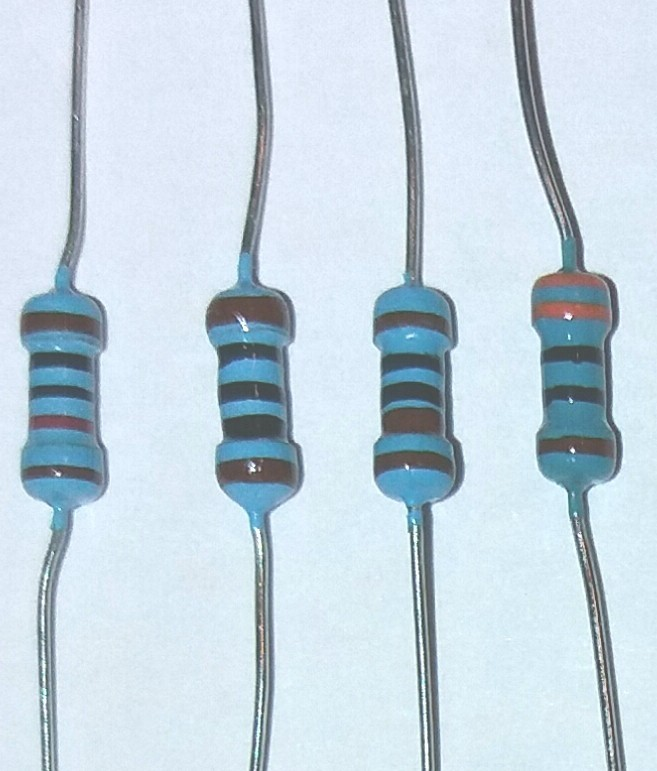
\includegraphics[width=0.18\textwidth,angle=90]{pics/Widerstaende.jpg}
	\vspace{-3\baselineskip}
	\label{abb:widerstaende}
\end{wrapfigure}
Bisher war die Größe des Vorwiderstands von LEDs mit $\SI{330}{\SIUnitSymbolOhm}$ vorgegeben. 
In unserem Bausatz finden sich jedoch viele weitere Widerstände, die teilweise größer und teilweise kleiner sind.

\begin{ziel}
	\textbf{Frage:} Welche Auswirkung haben Widerstände auf den Stromkreis? Wie kann man dies berechnen?
\end{ziel}

\begin{minipage}{0.58\textwidth}
	\begin{aufgabe} \emph{Zusammenhang von Widerstand, Stromstärke und Spannung}
		
		Rechts ist eine einfache Reihenschaltung mit einer Spannungsquelle, einer LED und einem Vorwiderstand abgebildet. Stelle eine Vermutung an, ob die LED heller oder dunkler leuchten wird, wenn man den Vorwiderstand verkleinert. Begründe deine Vermutung.
	\end{aufgabe}
	\vspace{3\baselineskip}
\end{minipage}
\hfill
\begin{minipage}{0.38\textwidth}
	\begin{figure}[H]
		\centering
		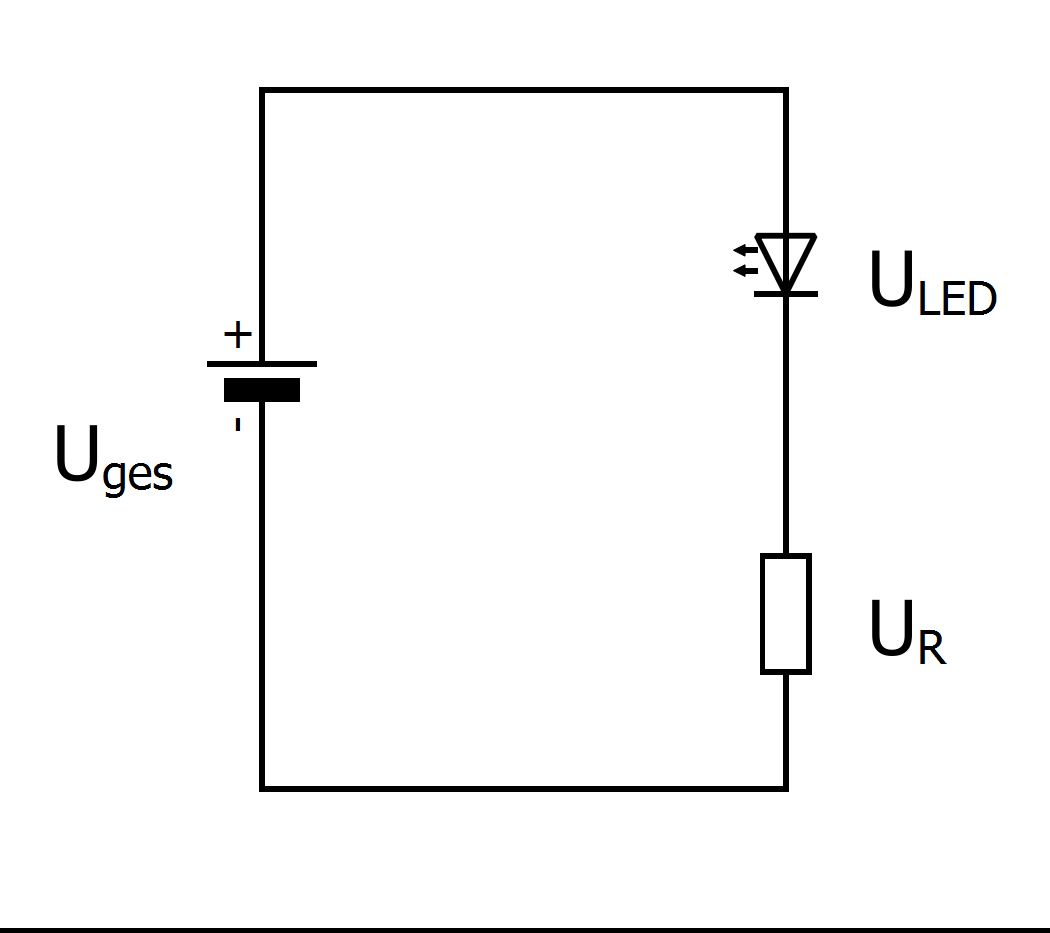
\includegraphics[width=\textwidth]{./Zeichnungen/ReiheLEDWiderstand.png}
		\caption{Reihenschaltung von LED und Vorwiderstand an einer Spannungsquelle.}
		\label{abb:reiheledwiderstand}
	\end{figure}
\end{minipage}

% Vorüberlegungen zur gleichzeitigen Wiederholung der Gesetze für die Reihenschaltung:
% Der Strom durch den Widerstand wird kleiner, wenn der Widerstand größer wird. Da die Stromstärke überall gleich groß ist, wird auch die Stromstärke in der LED kleiner.
% Die LED leuchtet, weil sie elektrische Energie in Lichtenergie umwandelt. Ein Maß für die elektrische Energie der Teilchen ist die Spannung. Wenn der Widerstand größer wird, wird auch die Spannung, die dort abfällt, größer (die Teilchen brauchen mehr Energie, um hindurch zu kommen). Daher wird die Spannung an der LED kleiner, denn die Gesamtspannung von 5V bleibt gleich und beide Spannungen addieren sich zur Gesamtspannung.
% Die Widerstände der Bauteile addieren sich ebenfalls zum Gesamtwiderstand.

\begin{aufgabe} \emph{Mindestgröße des Vorwiderstands}
	
	Berechne, wie groß der Vorwiderstand einer LED mindestens sein muss, damit sie nicht durchbrennt.
\end{aufgabe}

\emph{Hinweise:} \vspace{-0.5\baselineskip}
\begin{itemize}[itemsep=0mm,parsep=0mm]
	\item Wenn ein Digitalpin angeschaltet wird (zum Beispiel durch die Anweisung \texttt{schalte LED an} oder \texttt{schreibe digitalen Wert ... 1}), dann gibt er eine Spannung von 5V gegenüber GND aus.
	\item Durch eine LED darf höchstens ein Strom von $\SI{20}{\milli\ampere}$ fließen.
	\item Je nach Farbe halten LEDs eine andere maximale Spannung aus:
	
	\smallskip
	\begin{tabular}{l|l|l|l}
		Farbe & rot & gelb/grün & blau/weiß \\ \hline
		$U_{LED}$ & 1,6\,V - 2,2\,V & 1,9\,V - 2,5\,V & 2,7\,V - 3,5\,V \\
	\end{tabular}
\end{itemize}

\begin{zsfg}{{Widerstand, Spannung und Stromstärke}}
	\begin{wrapfigure}{r}{0.15\textwidth}
		\vspace{-\baselineskip}
		
\begin{tikzpicture}
		\draw [black, thick] (0,0) -- (0.8,1.5) -- (1.6,0) -- (0,0);
		\node at (0.8,0.9) {\color{black}$U$};
		\draw [black, thick] (0.5,0.6) -- (1.1,0.6);
		\node at (0.5,0.2) {\color{black}$R$};
		\node at (1.1,0.2) {\color{black}$I$};
		\end{tikzpicture}
	\end{wrapfigure}
	Der Widerstand $R$ ist definiert als das Verhältnis von Spannung $U$ zu Stromstärke $I$:
	\begin{equation*}
		R=\frac{U}{I}.
	\end{equation*}
	
	Ein Widerstand heißt \emph{ohmscher Widerstand}, wenn das Verhältnis $\frac{U}{I}$ stets gleich groß ist (also wenn $R$ unabhängig von Stromstärke und Spannung konstant ist).
\end{zsfg}
\begin{tcolorbox}[equal height group=A,enhanced, colback=CadetBlue!70!green, coltext=black, colframe=DarkCyan!70!DarkGreen, width=0.48\textwidth, before=, after=\hfill, adjusted title={Elektrische Stromstärke und Spannung in der Reihenschaltung}, colbacktitle=CadetBlue!70!green, coltitle=black, fonttitle=\bfseries]
	\begin{figure}[H]
		\centering
		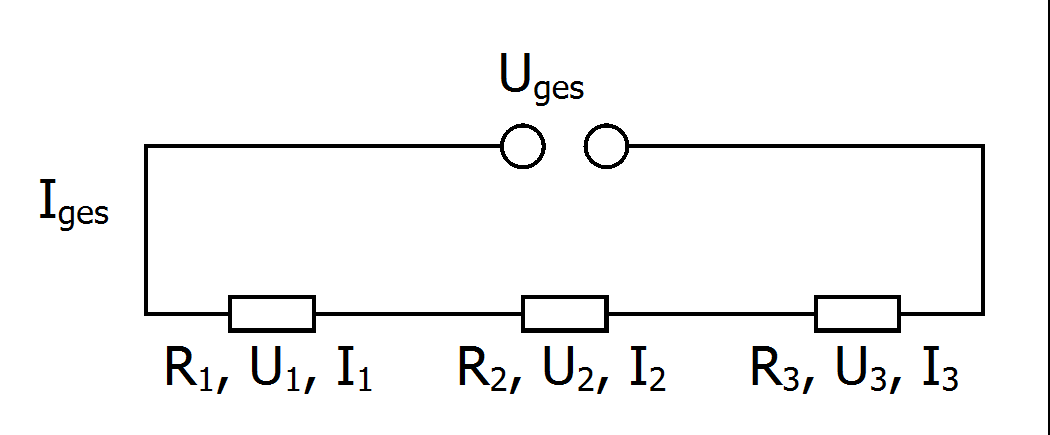
\includegraphics[width=\textwidth]{./Zeichnungen/reihenschaltung.png}
	\end{figure}
	\begin{itemize}[parsep=0ex,itemsep=0ex,leftmargin=*]
		\item In einer Reihenschaltung ist die Stromstärke an jeder Stelle gleich groß:
		\begin{equation*}
			I_{ges}=I_1=I_2= I_3=\dots
		\end{equation*}
		\item In einer Reihenschaltung teilt sich die Gesamtspannung auf die einzelnen Bauteile auf:
		\begin{equation*}
			U_{ges}=U_1 + U_2 + U_3+\dots
		\end{equation*}
		\item In einer Reihenschaltung addieren sich die Einzelwiderstände zum Gesamtwiderstand:
		\begin{equation*}
			R_{ges}=R_1+R_2+R_3+\dots
		\end{equation*}
	\end{itemize}
\end{tcolorbox}
\begin{tcolorbox}[equal height group=A,enhanced, colback=CadetBlue!70!green, coltext=black, colframe=DarkCyan!70!DarkGreen, width=0.48\textwidth, before=, after=\hfill, adjusted title={Elektrische Stromstärke und Spannung in der Parallelschaltung}, colbacktitle=CadetBlue!70!green, coltitle=black,fonttitle=\bfseries]
	\begin{figure}[H]
		\centering
		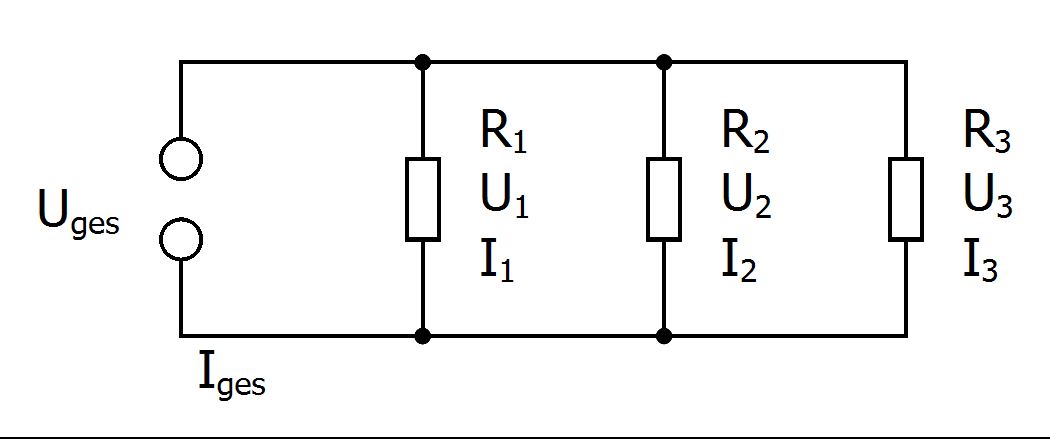
\includegraphics[width=\textwidth]{./Zeichnungen/parallelschaltung.png}
	\end{figure}
	\begin{itemize}[parsep=0ex,itemsep=0ex,leftmargin=*]
		\item In einer Parallelschaltung teilt sich die Gesamtstromstärke auf die einzelnen Zweige auf:
		\begin{equation*}
			I_{ges}=I_1+I_2+ I_3+\dots
		\end{equation*}
		\item In einer Parallelschaltung ist die Spannung in jedem Zweig gleich groß:
		\begin{equation*}
			U_{ges}=U_1=U_2=U_3=\dots
		\end{equation*}
		\item In einer Parallelschaltung ist der Kehrwert des Gesamtwiderstands gleich der Summe der Kehrwerte der einzelnen Widerstände:
		\begin{equation*}
			\frac{1}{R_{ges}} = \frac{1}{R_1} + \frac{1}{R_2} + \frac{1}{R_3} + \dots
		\end{equation*}
	\end{itemize}
\end{tcolorbox}

\begin{aufgabe}
	
	Unter den Bauteilen im Arduino-Kasten befindet sich auch ein 9V Akku. Berechne den mindestens notwendigen Vorwiderstand, wenn eine
	rote LED an den 9V Block angeschlossen wird.
\end{aufgabe}

\begin{aufgabe}
	\begin{enumerate}[label=\alph*), itemsep=0ex, parsep=0ex]
		\item An einem 9V Block sollen drei rote LEDs in Reihe geschaltet betrieben werden. Zeichne einen Schaltplan und berechne den passenden Vorwiderstand.
		\item An einem 9V Block sollen drei rote LEDs parallel geschaltet betrieben werden. Zeichne einen Schaltplan und berechne den passenden Vorwiderstand.
	\end{enumerate} 
\end{aufgabe}
\vfill

\newpage

\begin{aufgabe} \emph{Ampelschaltung}
	
	Max überlegt sich, dass er für eine Ampelschaltung am Arduino denselben Vorwiderstand für drei parallel geschaltete LEDs verwenden kann, sodass er nur einen Widerstand heraussuchen muss. Die Berechnung der Mindestgröße nimmt er folgendermaßen vor.
	
	\begin{tcolorbox}[sharp corners, colframe= white]
		\begin{wrapfigure}{r}{0.4\textwidth}
			\centering
			\vspace{-\baselineskip}
			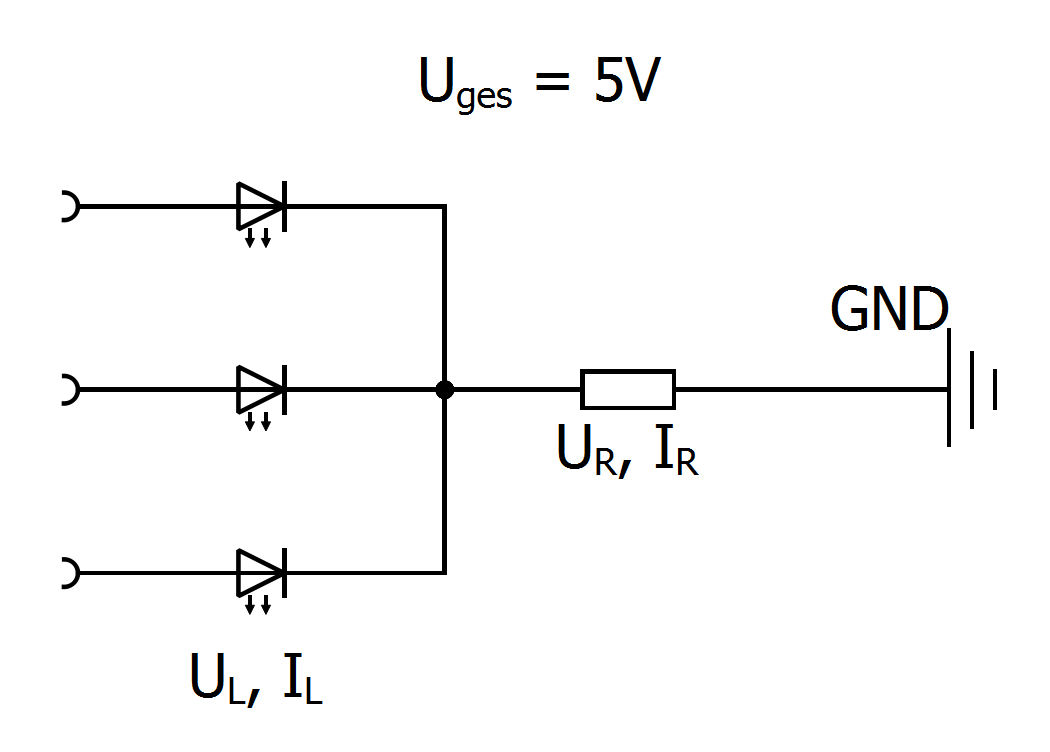
\includegraphics[width=0.4\textwidth]{./Zeichnungen/schaltplan-rgb-led-berechnung.png}
		\end{wrapfigure}
		$I_L = \SI{20}{\milli\ampere} = \SI{0,02}{\ampere} \quad \Longrightarrow \quad I_R = \SI{0,06}{\milli\ampere}$
		
		$U_L = \SI{2,2}{\volt}$ \quad (max. Spannung, die rote LEDs aushalten)
		
		$U_R = \SI{5}{\volt} - \SI{2,2}{\volt} = \SI{2,8}{\volt}$
		
		\begin{equation*}
			R = \frac{U_R}{I_R} = \frac{\SI{2,8}{\volt}}{\SI{0,06}{\ampere}} \approx \SI{46,67}{\ohm}
		\end{equation*}
		
		\bigskip
		Der Vorwiderstand sollte eine Größe von mindestens $\SI{50}{\ohm}$ haben.
	\end{tcolorbox}
	
	%Das Problem ist, dass auch nur eine LED angeschaltet sein kann und dann darf der Gesamtwiderstand nur 0,02 A durchlassen, muss also größer sein.
	
	\medskip
	Begründe, warum der oben berechnete Vorwiderstand zu niedrig ist. Erkläre, wie man stattdessen vorgehen müsste und gib den korrekten Wert für einen möglichen gemeinsamen Vorwiderstand an.
\end{aufgabe}

\bigskip
\begin{aufgabe} \emph{Vorbereitungen zur 7-Segment-Anzeige}
	\begin{enumerate}[label=\alph*), itemsep=0ex,parsep=0mm]
		\item Zeichne einen vereinfachten Schaltplan einer 7-Segment-Anzeige, %
		\marginpar{%
			\textattachfile[description={Druckvorlage zu Kap. \thechapter, Schaltplan mit Arduino}]{./Zeichnungen/Schaltplan-Arduino-Vorlage.pdf}{
				\footnotesize%
				\drucker Vorlage%
			}%
			\footnotesize%
			\\öffnen%
		}
		in dem die LEDs einzeln eingezeichnet sind (siehe Infokasten unten).
		\item Es wäre sehr umständlich, für jede LED einen eigenen Vorwiderstand anzuschließen; praktischer ist es, einen einzigen Vorwiderstand zwischen GND-Anschluss der 7-Segment-Anzeige und GND-Anschluss des Arduino anzubringen. Die Größe des gemeinsamen Vorwiderstands der acht LEDs (Anzeige \& Punkt) soll $\SI{330}{\ohm}$ betragen. Berechne die Gesamtstromstärke und die Stromstärke in jeder LED bei Darstellung einer 1 und einer 8 (jeweils ohne Punkt).
	\end{enumerate}
\end{aufgabe}

\begin{zsfg}{7-Segment-Anzeige}
	\begin{minipage}{0.58\textwidth}
		Eine 7-Segment-Anzeige besteht aus sieben roten LEDs, die so angeordnet sind, dass sich mit ihnen eine Zahl darstellen lässt. Zusätzlich gibt es  zur leichteren Unterscheidung von 6 und 9 eine LED für den Punkt. \emph{Jede LED lässt sich einzeln über einen der Pins ansteuern, wobei sich alle LEDs einen gemeinsamen GND-Anschluss teilen.} Der zweite GND-Anschluss soll hier nicht genutzt werden, um die Schaltung so einfach wie möglich zu halten.
		
		\vspace{2\baselineskip}
	\end{minipage}
	\hfill
	\begin{minipage}{0.4\textwidth}
		%		\begin{figure}[H]
		\hfill
		\begin{minipage}{0.48\textwidth}
			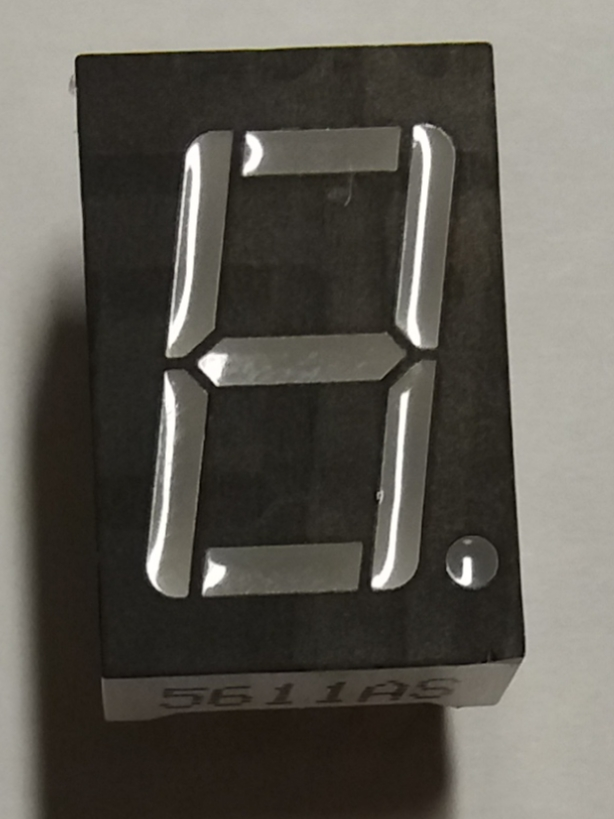
\includegraphics[width=\textwidth]{./pics/7segmentanzeige-bild2.jpg}
			%				\caption{7-Segment-Anzeige}
			%				\label{abb:7segment-bild}
		\end{minipage}
		\hfill
		\begin{minipage}{0.48\textwidth}
			\vspace{-0.2\baselineskip}
			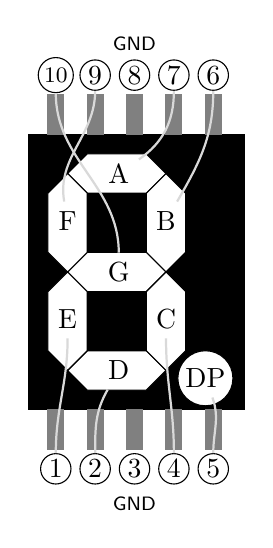
\begin{tikzpicture}[scale=0.5]
	% Rahmen der Anzeige
	\draw [fill=black] (0,0) rectangle (5.5,7);
	% Segment D
	\draw [fill = white] (1,1) -- ++(0.5,-0.5) -- ++ (1.5,0) -- ++ (0.5,0.5) -- ++ (-0.5,0.5) -- ++ (-1.5,0) -- ++(-0.5,-0.5)  node at ++(1.3,0) (segD) {D}; 
	% Segment G
	\draw [fill = white] (1,3.5) -- ++(0.5,-0.5) -- ++ (1.5,0) -- ++ (0.5,0.5) -- ++ (-0.5,0.5) -- ++ (-1.5,0) -- ++(-0.5,-0.5)  node at ++(1.3,0) (segG) {G};
	% Segment A
	\draw [fill = white] (1,6) -- ++(0.5,-0.5) -- ++ (1.5,0) -- ++ (0.5,0.5) -- ++ (-0.5,0.5) -- ++ (-1.5,0) -- ++(-0.5,-0.5)  node at ++(1.3,0) (segA) {A};
	% Segment E
	\draw [fill = white] (1,1) -- ++ (0.5,0.5) -- ++ (0,1.5) -- ++ (-0.5,0.5) -- ++ (-0.5,-0.5) -- ++ (0,-1.5) -- ++ (0.5,-0.5) node at ++ (0,1.3) (segE) {E};  
	% Segment C
	\draw [fill = white] (3.5,1) -- ++ (0.5,0.5) -- ++ (0,1.5) -- ++ (-0.5,0.5) -- ++ (-0.5,-0.5) -- ++ (0,-1.5) -- ++ (0.5,-0.5) node at ++ (0,1.3) (segC) {C};
	% Segment F
	\draw [fill = white] (1,3.5) -- ++ (0.5,0.5) -- ++ (0,1.5) -- ++ (-0.5,0.5) -- ++ (-0.5,-0.5) -- ++ (0,-1.5) -- ++ (0.5,-0.5) node at ++ (0,1.3) (segF) {F};
	% Segment B
	\draw [fill = white] (3.5,3.5) -- ++ (0.5,0.5) -- ++ (0,1.5) -- ++ (-0.5,0.5) -- ++ (-0.5,-0.5) -- ++ (0,-1.5) -- ++ (0.5,-0.5) node at ++ (0,1.3) (segB) {B};
	% Punkt DP
	\draw [fill = white] (4.5,0.8) circle [radius=0.7cm] node (segDP) {DP};
	% Kontaktstifte
	\foreach \x in {0.5, 1.5, ..., 4.5} {
		\draw [draw=gray, fill=gray] (\x,0) rectangle ++(0.4,-1);
		\draw [draw=gray, fill=gray] (\x,7) rectangle ++(0.4,1);
	}
	% Nummerierung der Kontaktstifte
	\node at (1-0.3,-1.5) [circle, draw, inner sep=1pt] (pin1) {1};
	\node at (2-0.3,-1.5) [circle, draw, inner sep=1pt] (pin2) {2};
	\node at (3-0.3,-1.5) [circle, draw, inner sep=1pt] (pin3) {3};
	\node at (4-0.3,-1.5) [circle, draw, inner sep=1pt] (pin4) {4};
	\node at (5-0.3,-1.5) [circle, draw, inner sep=1pt] (pin5) {5};
	%	\foreach \x in {9,...,6}{
	%		\node at (11-\x-0.3,8.5) [circle, draw, inner sep=1pt] {\x};
	%	}
	\node at (1-0.3,8.5) [circle, draw, inner sep=1pt] (pin10) {\footnotesize 10};
	\node at (11-9-0.3,8.5) [circle, draw, inner sep=1pt] (pin9) {9};
	\node at (11-8-0.3,8.5) [circle, draw, inner sep=1pt] (pin8) {8};
	\node at (11-7-0.3,8.5) [circle, draw, inner sep=1pt] (pin7) {7};
	\node at (11-6-0.3,8.5) [circle, draw, inner sep=1pt] (pin6) {6};
	\node at (2.7,-2.4) {\scriptsize\sffamily GND};
	\node at (2.7,9.3) {\scriptsize\sffamily GND};
	% Verbindungen
	\draw [gray!30!white, thick] (segA) to [out=35,in=270] (pin7); %out= Winkel beim Verlassen, in = Winkel beim Eintreffen
	\draw [gray!30!white, thick] (segB) to [out=60,in=270] (pin6);
	\draw [gray!30!white, thick] (segC) to [out=-90,in=90] (pin4);
	\draw [gray!30!white, thick] (segD) to [out=-120,in=90] (pin2);
	\draw [gray!30!white, thick] (segE) to [out=-90,in=90] (pin1);
	\draw [gray!30!white, thick] (segF) to [out=100,in=270] (pin9);
	\draw [gray!30!white, thick] (segG) to [out=90,in=270] (pin10);
	\draw [gray!30!white, thick] (segDP) to [out=-70,in=90] (pin5);
\end{tikzpicture}
			%				\caption{Pin-Diagramm der 7-Segment-Anzeige.}
			%				\label{abb:7segment-pins}
			\vspace{-1.5\baselineskip}
		\end{minipage}
		\hfill
		%		\end{figure}
	\end{minipage}
\end{zsfg}

\begin{projekt}[Raketencountdown]\label{proj:raketencountdown}
	Suche dir nun den passenden Widerstand für die 7-Segment-Anzeige heraus und verbinde beide mit dem Arduino. Programmiere dann einen Raketencountdown, der von 9 rückwärts bis 0 zählt.
	
	\emph{Tipp:} Erstelle dir zuerst eine Tabelle, in der du übersichtlich festhälst, welche LEDs für welche Zahl an sein müssen und mit welchen Pins am Arduino diese verbunden sind.
	
	\emph{Für Schnelle:} Man kann mit einer 7-Segment-Anzeige auch Buchstaben darstellen und nacheinander durchlaufen lassen!
	
	{\scriptsize Idee: Frick, Fritsch und Trick (2015): \emph{Einführung in Mikrocontroller - Der Arduino als Steuerzentrale}, Bad Saulgau}
\end{projekt}
\marginpar{
	\vspace{-4\baselineskip}
	\zurueck%
	\footnotesize
	\hyperref[sec:widerstandsringe]{Widerstandsringe\\ ablesen}%
}

%Beurteile anhand des unten abgebildeten Informationskastens, ob man die 7-Segment-Anzeige gefahrlos mit nur einem Vorwiderstand an den Arduino anschließen darf.
%\begin{zsfg}{Kennwerte zur maximalen Stromausgabe und Stromaufnahme}
%	
%	Wenn die angegebenen Maximalwerte überschritten werden, wird der Arduino Schaden nehmen!
%	\begin{itemize}[itemsep=0ex]
%		\item Max. Stromausgabe an Digitalpins: $\SI{40}{\milli\ampere}$ (empfohlen: $\SI{20}{\milli\ampere}$)
%		\item Max. Stromausgabe am VCC-Pin: $\SI{200}{\milli\ampere}$
%		\item Max. Stromaufnahme am GND-Pin: $\SI{200}{\milli\ampere}$
%	\end{itemize}
%\end{zsfg}
%\begin{flushright}
%	\vspace{-\baselineskip}
%	\footnotesize
%	Quelle: \url{https://playground.arduino.cc/Main/ArduinoPinCurrentLimitations}
%\end{flushright}


\section{Das elektrische Potential}
\label{sec:elektrisches-potential}

Die Ausgabe von 5\,V gegenüber GND an einem digitalen Ausgang des Arduino ist vergleichbar mit einer Batterie oder einem Spannungsgerät. Um zu verstehen, wie der Arduino digitale Signale einliest und dadurch auf seine Umwelt reagieren kann, muss jedoch zuerst geklärt werden, was sich hinter dem \emph{elektrischen Potential} verbirgt.

\begin{ziel}
	\textbf{Frage:} Wie werden digitale Signale am Arduino eingelesen?
\end{ziel}

\marginpar{%
	\textattachfile[description={Folie zu Kap. \thechapter, El. Potential}]{./Auftraege/kap4-auftrag-potential.pdf}{%
		\footnotesize\folie Folie%
	}%
	\footnotesize%
	%	\folie \href{run:./Auftraege/kap3-auftrag-potential.pdf}{Folie}%
	\\öffnen
}
\begin{aufgabe} \emph{Eine Analogie für das elektrische Potential}
	
	\begin{enumerate}[label=\alph*), itemsep=0ex, parsep=0ex]
		\item Anna und Bert schauen auf dasselbe Fenster. %
		Anna meint, das Fenster befinde sich in 1 Meter Höhe. Bert hingegen meint, das Fenster befinde sich in 4 Meter Höhe. Beide haben jeweils für sich betrachtet Recht. Wie kann das sein?
		\item Die Vase fällt einen Meter tief. Gib an, \dots
		\begin{itemize}[itemsep=0ex]
			\item \dots mit welcher Höhe Anna die Höhenenergie nach dem Fallen berechnet und mit welcher Höhendifferenz sie die Höhenenergie berechnet, die in Bewegungsenergie umgewandelt wurde.
			\item \dots mit welcher Höhe Bert die Höhenenergie nach dem Fallen berechnet und mit welcher Höhendifferenz er die Höhenenergie berechnet, die in Bewegungsenergie umgewandelt wurde.
		\end{itemize}
		
		Hinweis: $E_H=m\cdot g\cdot h$
	\end{enumerate}
\end{aufgabe}

%Lösung: Bei der Berechnung der Höhenenergie muss stets festgelegt werden, wo das \emph{Nullniveau} ist; das bedeutet: Wo die Höhe gemessen wird. Damit wird festgelegt: Bei dieser Grundhöhe ist die Höhenenergie null. Wenn nun eine Vase von der Fensterbank auf den Boden im Raum von Anna fällt, dann hat sie etwas Höhenenergie in Bewegungsenergie umgewandelt - und zwar genau die Höhenenergie, die einem Meter Höhendifferenz entspricht, denn sie ist einen Meter tief gefallen. \emph{Diese Differenz in der Höhe und der Höhenenergie ist unabhängig davon, welche Grundhöhe man betrachtet.} Sowohl aus Annas als auch aus Berts Sicht ist die Vase einen Meter tief gefallen.

\begin{aufgabe} \emph{Übersicht}
	
	\smallskip
	\begin{tabu} to \textwidth {X[L]X[L]}
		a) Übertrage und vervollständige die folgende Tabelle von Analogien.
		&
		b) Erkläre, welche der genannten Größen in der Mechanik bzw. der Elektrik abhängig von der Festlegung eines Nullniveaus sind.
		\\
	\end{tabu}
	
	\vspace{-0.5\baselineskip}
	\begin{minipage}{0.48\textwidth}
		\begin{tabular}{c|c}
			\textbf{Mechanik} & \textbf{Elektrik} \\ \hline
			Höhenenergie & \\ \hline
			& Elektrisches Potential \\ \hline
			Höhendifferenz & \\ \hline
			Grundhöhe & \\ \hline
		\end{tabular}
	\end{minipage}
	\hfill
\end{aufgabe}

%\vfill

\begin{zsfg}{Elektrisches Potential}
	\begin{minipage}{0.58\textwidth}
		So wie die Höhendifferenz ein Maß für die Höhenenergie ist, die umgewandelt wird (z. B. in Bewegungsenergie), ist die Spannung ein Maß für die elektrische Energie, die an einer LED, einem Widerstand etc. umgewandelt wird. 
		
		Das elektrische Potential hingegen ist wie die Höhe ein Maß für die elektrische Energie der Elektronen im Stromkreislauf. Es kann nur in Bezug auf ein Nullniveau (\enquote{Ground}/GND) angegeben werden. Die Einheit des elektrischen Potentials ist Volt.
		
		Elektrisches Potential am GND-Pin: 0V
		
		Elektrisches Potential am 5V-Pin: 5V
	\end{minipage}
	\hfill
	\begin{minipage}{0.4\textwidth}
		\begin{tikzpicture}
		%Hintergrund
		\fill [white] (-1,-0.5) rectangle (5.2,6);
		% x-Achse	
		\node at (0,0) [left] {\sffamily\scriptsize 0\,V };
		% y-Achse
		\draw [->] (0,-0.2) -- (0,5.2) node [below left=0.2mm] {\sffamily\scriptsize5\,V} node [above] {\sffamily\scriptsize El. Potential};
		\foreach \y in {1,2,3,4,5} {
			\draw (-0.1,\y) -- ++(0.2,0);
		}
		% Schaltplan
		\draw (0,0) circle [radius=0.1];
		\draw (0.1,0) -- (1,0);
		\draw (1,-0.2) rectangle ++(1.25,0.4); % Widerstand
		\draw (2.25,0) -- (3,0);
		\draw (3,-0.2) -- ++(0,0.4); % LED1
		\draw (3,0) -- ++(0.3,0.2) -- ++(0,-0.4) -- ++(-0.3,0.2); % LED2
		\draw [->] (3.1,0.2) -- ++(-0.1,0.1); %LED3
		\draw [->] (3.2,0.3) -- ++(-0.1,0.1); %LED4
		\draw (3.3,0) -- (4,0);
		\draw (4,0.2) -- ++(0,-0.4) ++(0.1,0.35) -- ++(0,-0.3) ++(0.1,0.25) -- ++(0,-0.2) ++ (0,0.1) node [right] {\sffamily\scriptsize GND}; % GND
		% Potentialverlauf
		\draw [color=blue] (0,5) -- (1,5) -- ++(1.25,-2.75) -- ++(0.75,0) -- ++(0.3,-2.25) -- ++(0.75,0);
		% Spannung am Widerstand markieren
		\draw [dashed] (2.25,5) -- ++(0.2,-0.2) -- ++(0,-2.35) -- ++(-0.2,-0.2) ++(0.2,1.375) -- ++(0.2,0) node [right, text width=2cm] {\sffamily\scriptsize Spannung am Widerstand};
		\end{tikzpicture}
	\end{minipage}
\end{zsfg}

\bigskip

\begin{aufgabe}\emph{Pulldown-Widerstand}
	
	In dem unten abgebildeten Schaltplan ist dargestellt, wie man einen Taster am Arduino so anschließt, dass man seinen Zustand im digitalen Pin 3 auslesen kann. Der Widerstand wird auch als \emph{Pulldown-Widerstand} bezeichnet und sollte relativ groß sein. $\SI{10}{\kilo\ohm}$ sind üblich.
	
	Markiere die Kabel farbig, sodass die Kabel, die auf dem gleichen elektrischen Potential liegen, die gleiche Farbe haben. Notiere zudem den Wert des elektrischen Potentials.
\end{aufgabe}
\marginpar{%
	\textattachfile[description={Druckvorlage zu Kap. \thechapter, El. Potential an Tastern}]{./Auftraege/kap4-druckvorlage-taster.pdf}{
		\footnotesize%
		\drucker Vorlage%
	}%
	\footnotesize%
	\\öffnen%
}

\begin{figure}[H]
	\hfill
	\begin{minipage}{0.4\textwidth}
		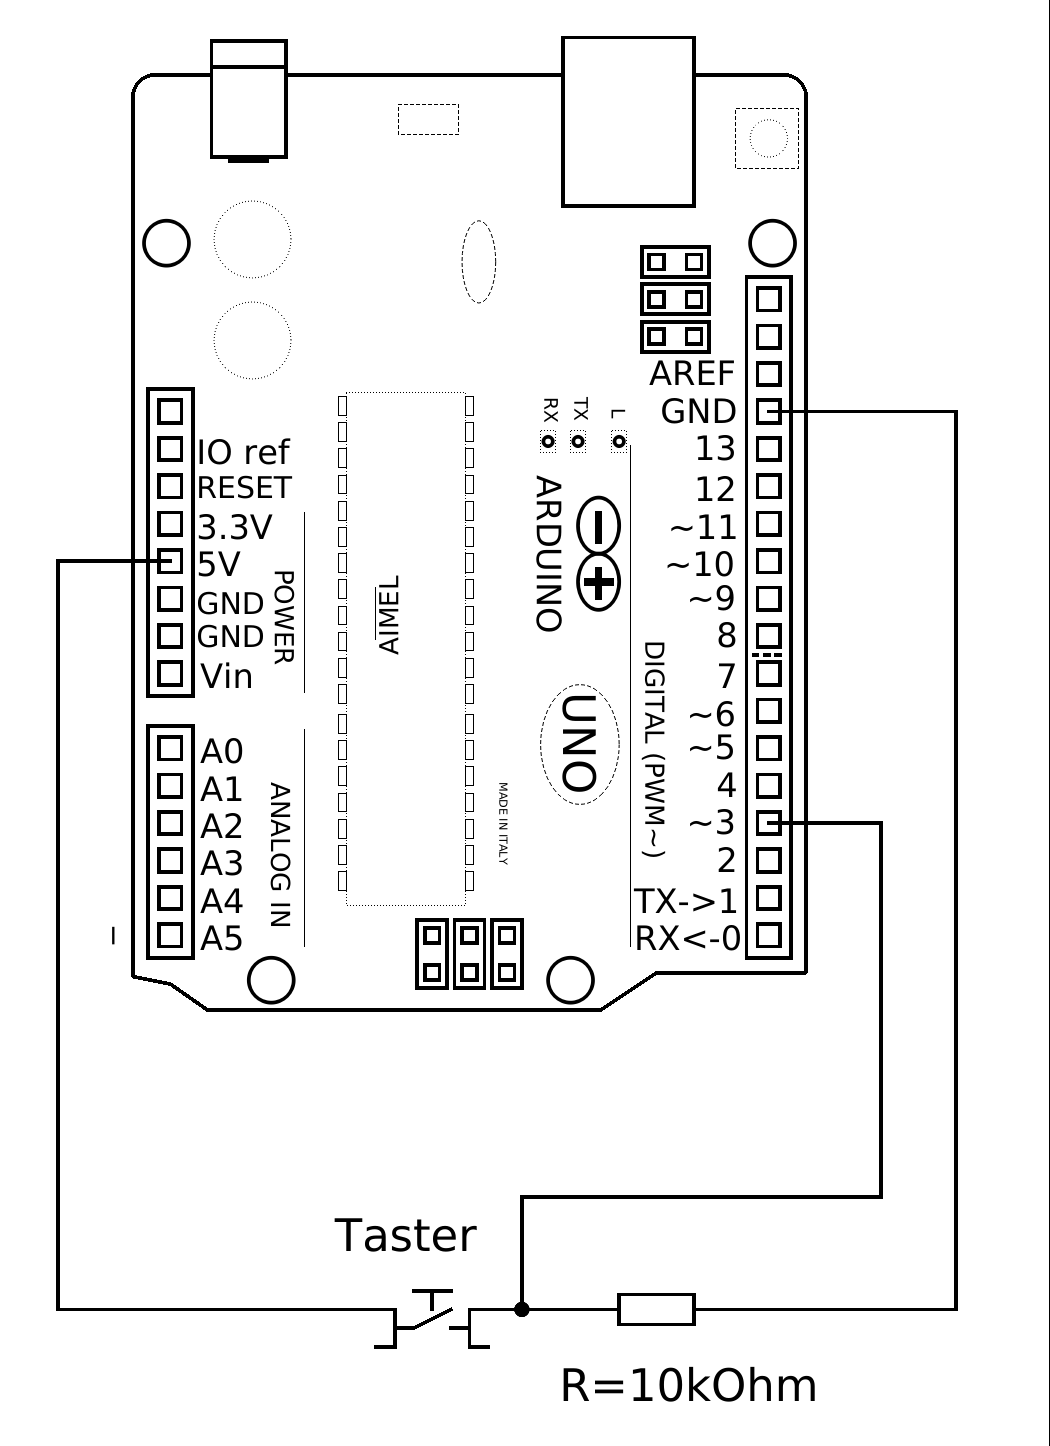
\includegraphics[width=0.8\textwidth]{./Zeichnungen/taster-an-arduino.png}
		\caption{Taster offen (kein Stromfluss).}
	\end{minipage}
	\hfill
	\begin{minipage}{0.4\textwidth}
		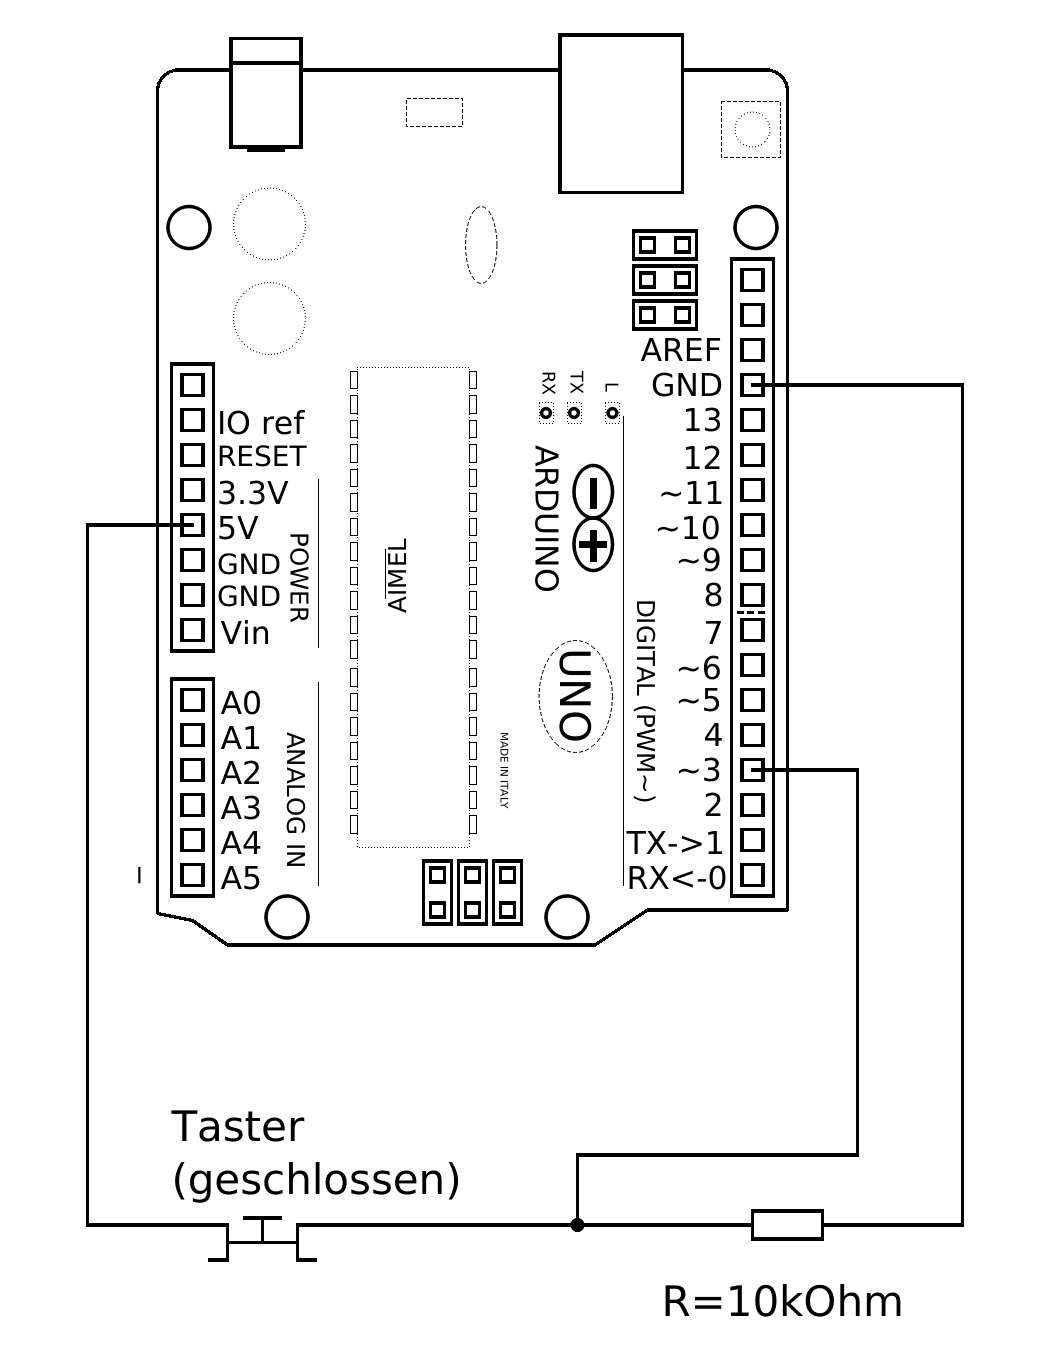
\includegraphics[width=0.8\textwidth]{./Zeichnungen/taster-an-arduino-geschlossen.png}
		\caption{Taster geschlossen (Stromfluss).}
	\end{minipage}
	\hfill
	\label{abb:schaltplan-taster-pulldown}
\end{figure}
\vfill

\begin{aufgabe} \emph{Pullup-Widerstand}
	
	Eine Alternative zu der bekannten oberen Schaltung ist die Schaltung mit einem sogenannten Pullup-Widerstand. In der Abbildung ist die Schaltung mit einem Taster und einem Pullup-Widerstand dargestellt.
	
	\begin{figure}[H]
		\centering
		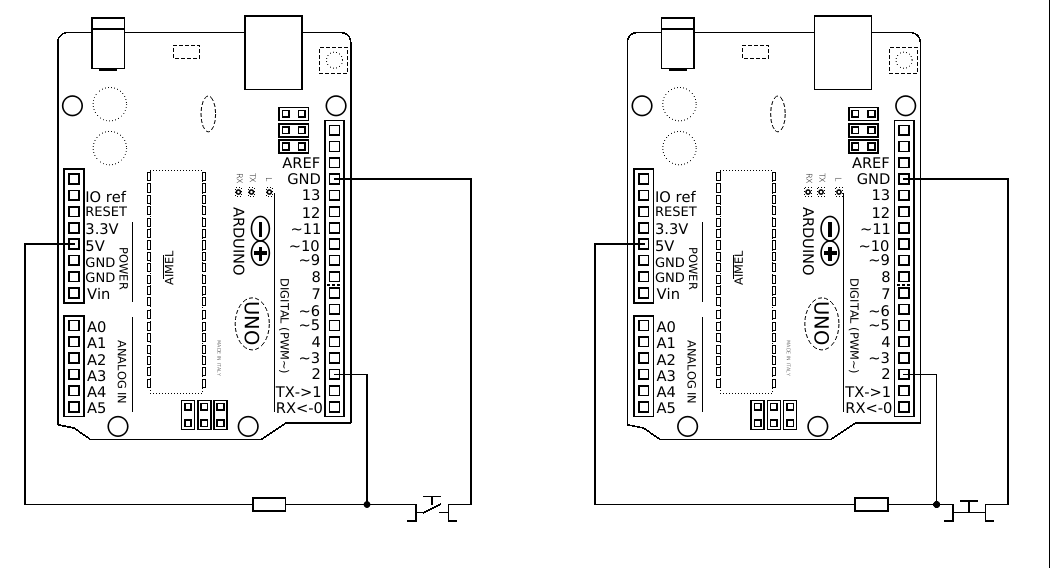
\includegraphics[width=0.8\textwidth]{./Zeichnungen/schaltplan-pullup.png}
	\end{figure}
	
	\begin{enumerate}[label=\alph*), itemsep=0ex, parsep=0ex]
		\item Markiere die Kabel jeweils farbig, sodass die Kabel, die auf dem gleichen elektrischen Potential liegen, die gleiche Farbe haben. Notiere zudem den Wert des elektrischen Potentials.
		\item Erläutere die Bedeutung der beiden Begriffe \emph{Pulldown} und \emph{Pullup}.
		
		\emph{Hinweis: to pull - engl. für \enquote{ziehen}}
	\end{enumerate}
\end{aufgabe}

\bigskip
\begin{projekt}[Fußgängerampel reloaded]\label{proj:fussampel2}
	Baue und programmiere eine Fußgängerampel mit einer Pullup-Schaltung für den Taster!
\end{projekt}

\bigskip
\begin{zsfg}{Digitale Pins des Arduino}
	\begin{minipage}{0.6\textwidth}
			Die digitalen Pins des Arduino von 0 bis 13 kennen nur zwei Zustände, für die es unterschiedliche Bezeichnungen gibt (siehe rechts). Sie können als digitaler Ausgang oder als digitaler Eingang konfiguriert werden. Bei einem digitalen Ausgang kann eine Spannung von 5\,V oder 0\,V gegenüber GND ausgegeben werden. Ein digitaler Eingang kann Spannungen zwischen 0\,V und 5\,V einlesen; dabei werden Spannungen von 0\,V bis 1,4\,V als \texttt{LOW} oder \texttt{0} interpretiert, größere Spannungen als \texttt{HIGH} oder \texttt{1}.
	\end{minipage}
	\hfill
	\begin{minipage}{0.35\textwidth}
		Bezeichnungen für Zustände von digitalen Pins
		
		\medskip
		\begin{center}
			\begin{tabular}{c|c} \hline
				An & Aus \\ \hline
				HIGH (5\,V) & LOW (0\,V) \\ \hline
				1 & 0 \\ \hline
			\end{tabular}
		\end{center}
		
		\medskip
		\scriptsize \emph{Hinweis: Bei vielen anderen Mikrocontrollern entspricht das HIGH-Potential 3,3\,V.}
	\end{minipage}
\end{zsfg}


\newpage
\section{Pulsweitenmodulation}
\label{sec:pwm}

\begin{ziel}
	\textbf{Ziel:} Mithilfe des Arduino soll eine funkelnde LED-Kerze gebaut werden.
\end{ziel}

\begin{wrapfigure}{r}{0.35\textwidth}
	\centering
	
\includegraphics[width=0.35\textwidth]{./pics/analogwrite.png}
\end{wrapfigure}
Der Arduino verfügt über mehrere sogenannte PWM-Pins, die mit einer Tilde ($\sim$) gekennzeichnet sind. Du hast diese Pins schon bei den analogen Aktoren kennen gelernt, weil diese über Pulsweitenmodulation (PWM) angesprochen werden. Die PWM-Werte, die der Anweisung übergeben werden können, variieren von 0 bis 255.

\bigskip

\begin{aufgabe} \emph{Fading}
	\begin{enumerate}[label=\alph*), itemsep=0ex, parsep=0ex]
		\item Schließe eine LED mit Vorwiderstand an einen PWM-Pin an und konfiguriere einen analogen Aktor an diesem Pin. Implementiere dann eine Zählschleife, die systematisch alle PWM-Werte von 0 bis 255 durchläuft. Beschreibe die Auswirkung auf die LED.
		\item Sorge dafür, dass die PWM-Werte nach Erreichen der 255 genauso rückwärts von 255 bis 0 durchlaufen werden.
		\item \emph{Zum Experimentieren:} Was passiert, wenn PWM-Werte größer als 255 übergeben werden?
	\end{enumerate}
\end{aufgabe}

\bigskip
\begin{aufgabe} \emph{Pulsweitenmodulation}
	
	Erkläre mithilfe der Zusammenfassung zur Pulsweitenmodulation, was bei der Nutzung des Befehls \button{Schreibe analogen Wert Aktor A 158} passiert. Berechne auch die mittlere Spannung, die am PWM-Pin ausgegeben wird.
	
	\emph{Für Physik-Profis:} Eine blaue LED hält bis zu 3,5\,V aus, ohne durchzubrennen. Trotzdem darf man sie bei Verwendung dieses Befehls nicht ohne Vorwiderstand an den Pin anschließen. Begründe.
\end{aufgabe}

\bigskip
\begin{projekt}[Kerzenfunkeln]\label{proj:kerzen}
	Modelliere mithilfe von drei LEDs das Funkeln von Kerzen.
	
	Tipp: Die Verwendung des Blocks für Zufallszahlen wird dir helfen, das Funkeln natürlicher aussehen zu lassen.
\end{projekt}

\vfill
\newpage

\begin{zsfg}{Pulsweitenmodulation (PWM)}
	
	\begin{wrapfigure}{r}{0.45\textwidth}
		\centering
		\begin{tikzpicture}[scale=0.8]
		\fill [white] (-1.2,-1.3) rectangle (7,7.1);
		\draw [->] (0,-0.6) -- (0,6.5);
		\draw [->] (-1,0) -- (6.5,0);
		\draw [dashed] (4,-1) -- ++(0,7.5);
		\node at (-0.2,-0.3) {\scriptsize 0};
		\foreach \x in {1,...,6} {
			\draw (\x,0.1) -- (\x,-0.1);% node [anchor=north, fill=white] {\scriptsize\x};
			\draw (0.1,\x) -- (-0.1,\x) node [anchor=east] {\scriptsize\x};
		}
		\node at (1,-0.1) [anchor=north, fill=white] {\scriptsize 5};
		\node at (3,-0.1) [anchor=north, fill=white] {\scriptsize 15};
		\node at (5,-0.1) [anchor=north, fill=white] {\scriptsize 25};
		\node at (6.5,-0.65) {\parbox{0.7cm}{\scriptsize Zeit in ms}};
		\node at (0,6.5) {\parbox{1.7cm}{\scriptsize El. Potential in V}};
		\draw [thick, blue] (0,5) -- ++(1,0) ++(0,-5) -- ++(3,0) ++(0,5) -- ++(1,0) ++(0,-5) -- ++(1.5,0);
		\draw [thick, red] (0,1.25) -- ++(6.5,0) node [above] {$\overline{U}$};
		\draw [<->] (0,-0.6) -- (4,-0.6) node [below left] {\scriptsize Periodendauer $T=\SI{20}{\milli\second}$};
		\end{tikzpicture}
		\caption{Darstellung des zeitlichen Verlaufs einer Pulsweitenmodulation mit einem Tastverhältnis von 25\%.}
	\end{wrapfigure}
	Bei der Pulsweitenmodulation wechselt der ausgewählte digitale Pin sehr schnell (mit einer Frequenz von 50\,Hz) zwischen den elektrischen Potentialen 5\,V und 0\,V hin und her - es ergibt sich also ein gepulstes Signal, dessen Weite (Dauer) moduliert werden kann. Aus dem Verhältnis der Zeit, in der der Pin auf einem 5\,V-Potential liegt, zu der Zeit, in der der Pin auf einem 0\,V-Potential liegt, ergibt sich eine mittlere Spannung (gegenüber Ground), die scheinbar am Pin anliegt. Wenn der Pin in der Hälfte der Zeit auf 5\,V und in der anderen Hälfte auf 0\,V liegt, dann ergibt sich eine mittlere Spannung von $\overline{U}=2,5\,V$. Wenn der Pin nur in einem Viertel der Zeit auf 5\,V liegt, dann ergibt sich eine mittlere Spannung von $\overline{U}=1,25\,V$ ($=5\,V\cdot 0,25$).
	
	Das Verhältnis der Zeit mit 5\,V zu der Gesamtdauer einer Periode mit 5\,V und 0\,V wird als \emph{Tastverhältnis} bezeichnet. Im Programm wird das Tastverhältnis durch einen Wert zwischen 0 und 255 angegeben. Eine 0 bedeutet, dass die Zeit mit 5\,V 0\% ausmacht, also liegt der Pin durchgängig auf einem 0\,V-Potential. Eine 255 bedeutet, dass die Zeit mit 5\,V 100\% ausmacht, also liegt der Pin durchgängig auf einem 5\,V-Potential. Diese beiden Werte entsprechen dem, was bei den bekannten Befehlen zur Steuerung von digitalen Pins passiert.
	
	Ein Wert von 100 bedeutet einen Anteil von $\frac{100}{255}\approx 0,39$ der Periodendauer. Daraus ergibt sich eine mittlere Spannung von $\overline{U}=5\,V\cdot 0,39\approx 1,96\,V$.
\end{zsfg}

\newpage
\section{Spannung messen}
\label{sec:spannung-messen}

Wenn Batterien kaum noch Ladung gespeichert haben, lässt die Spannung an ihren Polen nach und sinkt unter den Wert, der auf der Batterie vermerkt ist. Mithilfe der analogen Eingänge A0 bis A5 lässt sich die Spannung messen und so entscheiden, ob die Batterie noch brauchbar ist.
\marginpar{%
	\textattachfile[description={Arbeitsblatt zu Kap. \thechapter, Spannung messen}]{./Auftraege/kap4-batterietester.pdf}{
		\footnotesize%
		\drucker Vorlage%
	}%
	\footnotesize%
	\\öffnen%
}

\begin{ziel}
	\textbf{Frage:} Wie kann man mit dem Arduino eine Spannung messen?
\end{ziel}

\begin{projekt}[Batterietester (Voltmeter für $U<5\,V$)]\label{proj:batterietesterklein}
	\begin{wrapfigure}{r}{0.3\textwidth}
		\centering
		\vspace{-2\baselineskip}
		\begin{tabular}{c | c}\footnotesize
			\textbf{Analogwert} & \textbf{Spannung} \\ \hline
			0 & 0\,V \\ \hline
			1 &  \\ \hline
			100 &  \\ \hline
			1023 & 5\,V \\ \hline
		\end{tabular}
%		\vspace{-\baselineskip}
	\end{wrapfigure}
	Für eine einfache Messung bei einer 1,5\,V-Batterie wird der negative Pol der Batterie mit GND verbunden, sodass ein gemeinsames Nullpotential vorliegt. Der positive Pol der Batterie wird mit einem der analogen Eingänge A0 bis A5 verbunden. Über einen eingebauten Analog-Digital-Wandler (\emph{engl. analog-to-digital converter, ADC}) wird der Spannungswert durch eine Zahl zwischen 0 und 1023 ausgedrückt.
	
	\begin{enumerate}[label=\alph*), itemsep=0mm, parsep=0mm]
		\item Schließe eine mit 1,5\,V beschriftete Batterie an den Arduino an und miss die Spannung. Berechne aus dem Analogwert die Spannung und lass sie auf dem seriellen Monitor ausgeben.
		\item Ergänze den Batterietester um eine Ampel, die anzeigt, ob die Batterie voll aufgeladen bzw. noch in Ordnung bzw. leer ist.
	\end{enumerate}	
\end{projekt}

\begin{projekt}[Batterietester (Voltmeter für $U>5\,V$)]\label{proj:batterietestergross}
	Da der Arduino beim direkten Anschließen nur maximal 5\,V \enquote{verträgt}, muss man zum Testen von z.\,B. 9\,V-Blöcken weitere Bauteile verwenden. Mit zwei $\SI{10}{\kilo\ohm}$ Widerständen kann man einen einfachen \emph{Spannungsteiler} aufbauen, der die Messung ermöglicht.
	%\vspace{-\baselineskip}
	\begin{minipage}{\textwidth}
		\begin{minipage}{0.48\textwidth}
			\begin{enumerate}[label=\alph*), itemsep=0mm, parsep=0mm]
				\item Berechne die Stromstärke und die Spannung an den Widerständen. Warum sind große Widerstände hier sinnvoll?
				\item Markiere die Kabel in der Abbildung farbig, sodass die Kabel, die auf dem gleichen elektrischen Potential liegen, die gleiche Farbe haben. Notiere zudem den Wert des elektrischen Potentials.
			\end{enumerate}
		\end{minipage}
		\hfill
		\begin{minipage}{0.48\textwidth}
			\centering
			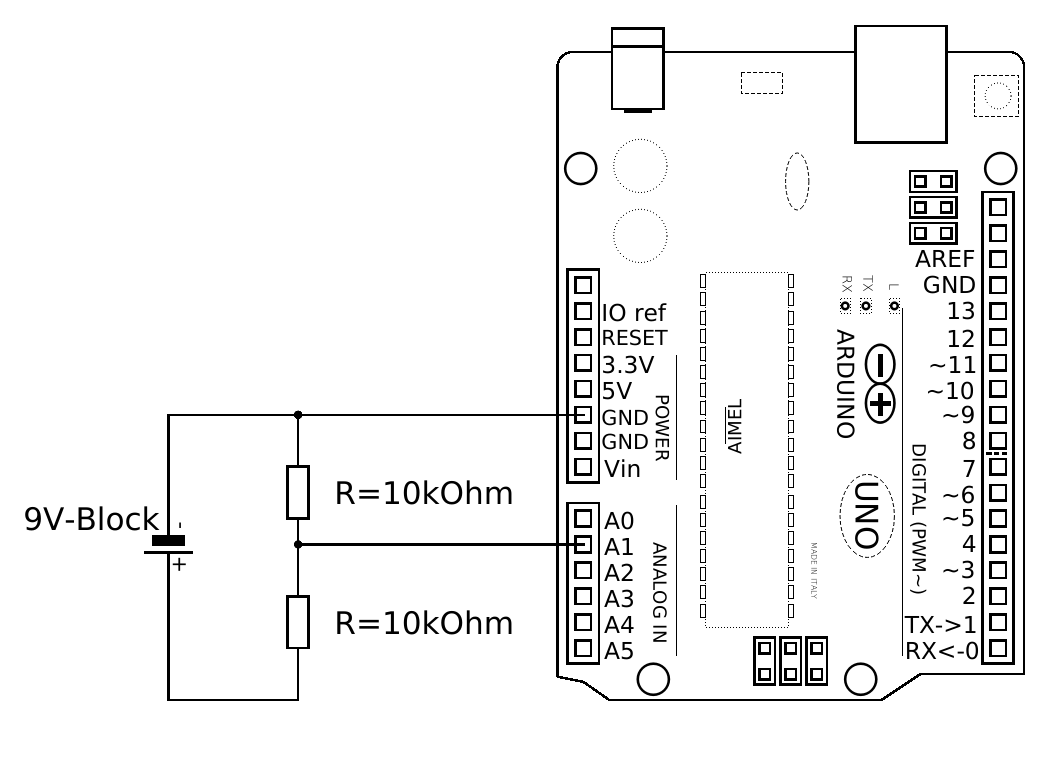
\includegraphics[width=0.95\textwidth]{./Zeichnungen/schaltplan-batterietester.png}
		\end{minipage}
	\end{minipage}
	\begin{enumerate}[label=\alph*), itemsep=0mm, parsep=0mm,start=3]
		\item Gib an, wie man mit dem Arduino die Spannung am 9\,V-Block berechnet. Baue den Batterietester dann auf und probiere ihn mit dem 9\,V-Block aus der Box aus.
		\item \emph{Zum Nachdenken:} Wie groß darf die Spannung beim oben verwendeten Spannungsteiler maximal sein, damit am Arduino nicht mehr als 5\,V anliegen? Wie könnte man den Spannungsteiler bauen, sodass man Spannungen bis zu 15\,V messen kann?
	\end{enumerate}
\end{projekt}

\bigskip
\begin{wrapfigure}{r}{0.2\textwidth}
	\centering
%	\vspace{-\baselineskip}
	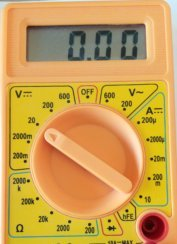
\includegraphics[width=0.15\textwidth]{./pics/multimeter.jpg}
	\caption{Einfaches Multimeter.}
	\vspace{-5\baselineskip}
\end{wrapfigure}
\emph{Hinweis:} Ganz ähnlich funktioniert ein Multimeter, bei dem man mit einem Drehregler ein passendes Widerstandsverhältnis für den aufgedruckten Messbereich einstellen kann. Auch im Multimeter werden für die Spannungsmessung möglichst große Widerstände verwendet.

\vspace{4\baselineskip}

\begin{zsfg}{(Quasi) Analoge Pins am Arduino}
	Die mit einer Tilde versehenen Digitalpins am Arduino verfügen über Pulsweitenmodulation, über die sich eine mittlere Spannung einstellen lässt, die quasi einem analogen Signal entspricht. Genau genommen sind 256 Stufen von 0 (0\,V) bis 255 (5\,V) möglich, woraus sich ergibt, dass die Stufen sich um 0,02\,V unterscheiden.
	
	Die Pins mit der Beschriftung A0 bis A5 werden als analoge Eingänge bezeichnet, weil sich mit ihnen Spannungen zwischen 0\,V und 5\,V messen lassen. Auch hier handelt es sich nur um eine quasi analoge Messung, denn der Messbereich ist in 1024 Stufen von 0 (0\,V) bis 1023 (5\,V) unterteilt, woraus sich ergibt, dass die Stufen sich um 0,005\,V unterscheiden.
\end{zsfg}

\newpage
%\newgeometry{twoside, top=2cm, outer=2.6cm, inner=2.6cm, % inner und outer sind aus irgendeinem Grund vertauscht
%	marginparwidth=2cm, marginparsep=0.3cm,% Die Breite für die Marginalien (Randbemerkungen) auf der rechten Seite
%	bottom=1cm, footskip=24pt, %Abstand zwischen Textboden und Fußzeilenboden
%	includefoot, includehead}
\section{Drehregler verwenden}
\label{sec:poti}

% Bleistiftpoti
Die Messung einer variablen, (quasi-)analogen Spannung eröffnet neue Möglichkeiten, da die Eingabewerte nun viel differenzierter sind als bei einem Taster, bei dem die Eingabe nur aus \enquote{0} oder \enquote{1} bestand. Zum Beispiel kann man darüber angeben, wie hell eine Lampe leuchten soll bzw. wie stark sie gedimmt werden soll. Dazu werden Potentiometer verwendet.

\begin{ziel}
	\textbf{Frage:} Wie funktioniert ein Potentiometer?
\end{ziel}
%\bigskip

\marginpar{%
	\textattachfile[description={Folie zu Kap. \thechapter, Bleistiftpotentiometer}]{./Auftraege/kap4-bleistiftpoti.pdf}{%
		\footnotesize\folie Folie%
	}
	\footnotesize%
	%\folie \href{run:./Auftraege/kap5-bleistiftpoti.pdf}{Folie} \\
	\\öffnen%
}
\begin{aufgabe}\emph{Bleistiftpotentiometer}
	
	\medskip
	\begin{minipage}{0.6\textwidth}
		Ein einfaches Potentiometer kannst du selbst bauen. 
		
		\smallskip
		\emph{Basteln:} Markiere dafür mit Bleistift einen dicken Strich auf einem Blatt Papier und klebe am einen Ende ein Kabel fest, das mit GND verbunden ist. Klebe ans andere Ende ein Kabel, das mit 5V verbunden ist. Mit einem dritten Kabel (\enquote{Sensorkabel}), das mit einem analogen Eingang verbunden ist, lässt sich nun messen, welches elektrische Potential an einer beliebigen Stelle des Bleistiftstreifens anliegt.
		
		\smallskip
		\emph{Experimentieren:}	Schreibe ein Programm, dass dir fortlaufend auf dem seriellen Monitor die Analogwerte und die umgerechneten Werte für das elektrische Potenzial bzw. die Spannung gegenüber GND anzeigt. Bewege dann das Sensorkabel über den Streifen und beobachte, wie sich die Spannungswerte verändern.
	\end{minipage}
	\hfill
	\begin{minipage}{0.39\textwidth}
		\centering
		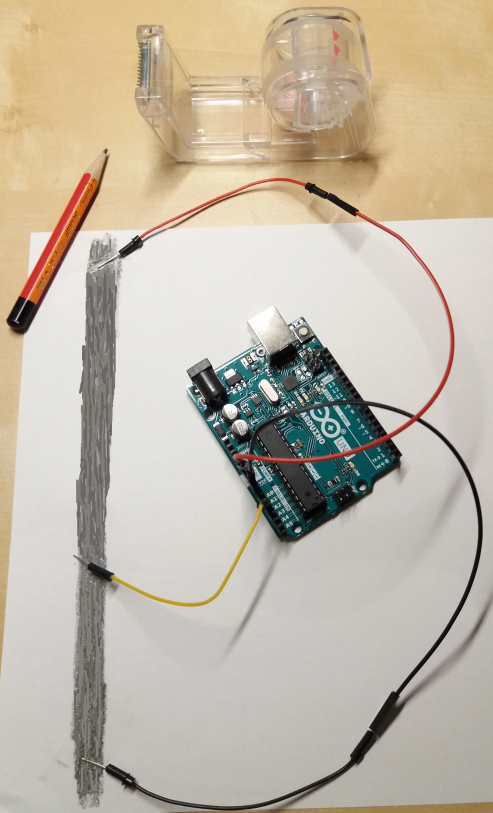
\includegraphics[width=0.75\textwidth]{./pics/bleistiftpoti-klein.png}
	\end{minipage}
	
	\medskip
	\emph{Analysieren:}	Der Bleistiftstreifen leitet den Strom bei einem bestimmten Gesamtwiderstand $R_{ges}$. Durch das Sensorkabel wird der Streifen in zwei Teile mit den Teilwiderständen $R_1$ und $R_2$ geteilt. Erläutere anhand deiner Beobachtungen, wie die drei Widerstände zusammenhängen.
	
	{\scriptsize Idee: Frick, Fritsch und Trick (2015): \emph{Einführung in Mikrocontroller - Der Arduino als Steuerzentrale}, Bad Saulgau}
\end{aufgabe}
\vfill

\begin{zsfg}{Potentiometer}
	\begin{minipage}{0.7\textwidth}
		Ein \textbf{Potentiometer}, kurz: Poti, ist im Grunde nichts anderes als ein Spannungsteiler mit zwei Widerständen. Jedoch kann die Größe der Widerstände z.\,B. durch Drehen variiert werden. Der Gesamtwiderstand bleibt dabei immer gleich.
	\end{minipage}
	\hfill
	\begin{minipage}{0.28\textwidth}
		\begin{minipage}{0.48\textwidth}
			\centering
			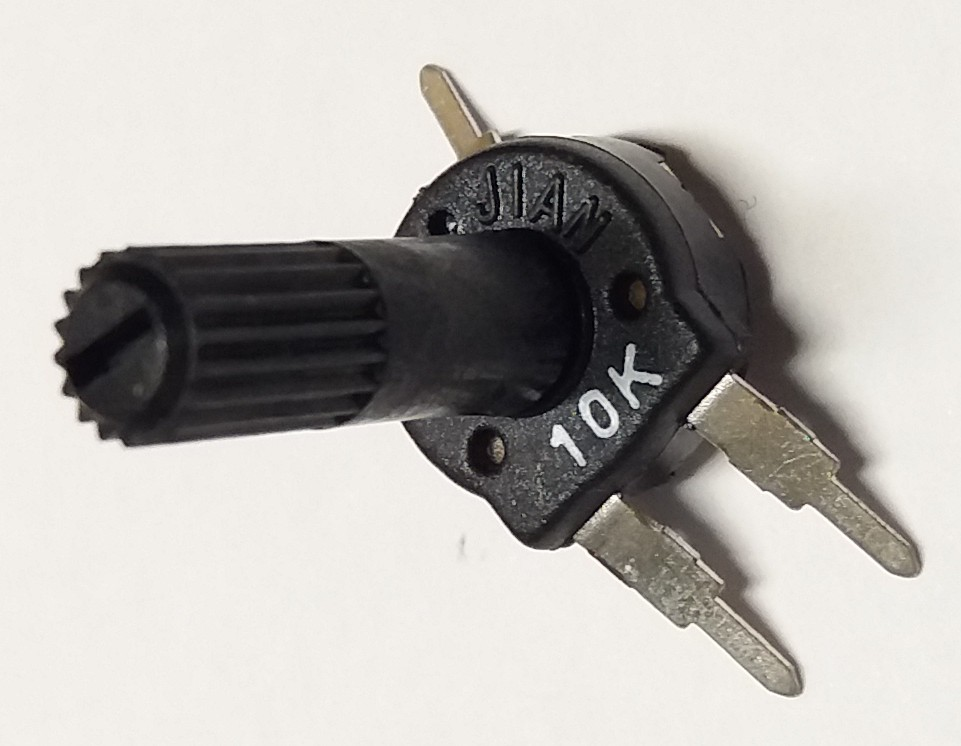
\includegraphics[angle=-90,width=0.8\textwidth]{./pics/poti.jpg}
		\end{minipage}
		\hfill
		\begin{minipage}{0.48\textwidth}
			\centering
			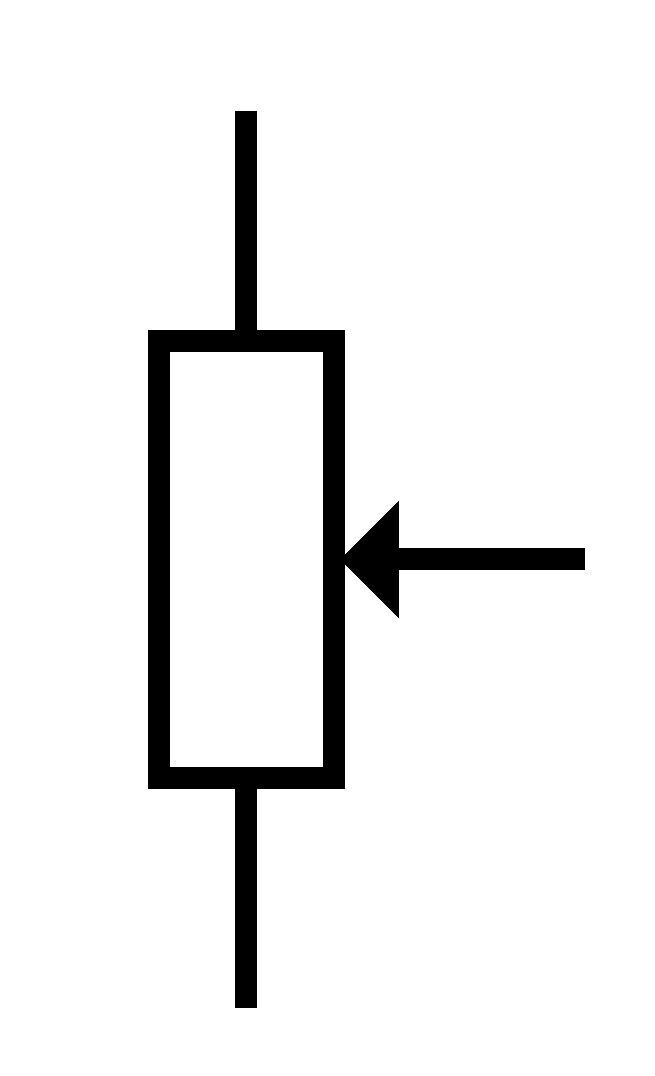
\includegraphics[width=0.65\textwidth]{./pics/poti-schaltsymbol.png}
		\end{minipage}
	\end{minipage}
	
	\smallskip
	Beim Anschluss an den Arduino wird der mittlere Pin des Potentiometers an einen analogen Eingang angeschlossen. Die anderen beiden Pins werden mit GND und 5V verbunden.
\end{zsfg}

\newpage
\begin{projekt}[Dimmbare Lampe]\label{proj:dimmlampe}
	Baue und programmiere eine Lampe, deren Helligkeit sich durch ein Potentiometer einstellen lässt.
	
	\begin{minipage}{0.8\textwidth}
		\emph{Hinweis:} Du musst dafür sorgen, dass der eingelesene Analogwert zwischen 0 und 1023 in einen PWM-Wert zwischen 0 und 255 umgerechnet wird. Ermittle dazu eine passende Funktion.
	\end{minipage}
	\hfill
	\begin{minipage}{0.19\textwidth}
		\centering
		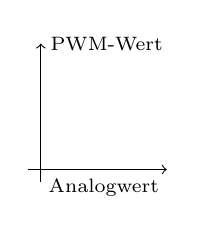
\begin{tikzpicture}[scale=0.8]
		\draw [->] (-0.2,0) -- (2,0);
		\draw [->] (0,-0.2) -- (0,2);
		\node at (1,0) [below] {\scriptsize Analogwert};
		\node at (0,2) [right] {\scriptsize PWM-Wert};
		\end{tikzpicture}
	\end{minipage}
\end{projekt}
%\restoregeometry
%\onehalfspacing

\subsection{Die Verwendung eines Potentiometers ohne Mikrocontroller}

Für einige Projekte, wie das Dimmen einer Lampe, ist ein Mikrocontroller eigentlich überdimensioniert, weil sich die Funktion schon durch eine reine Hardwarelösung erreichen lässt.

\begin{figure}[H]
	\centering
	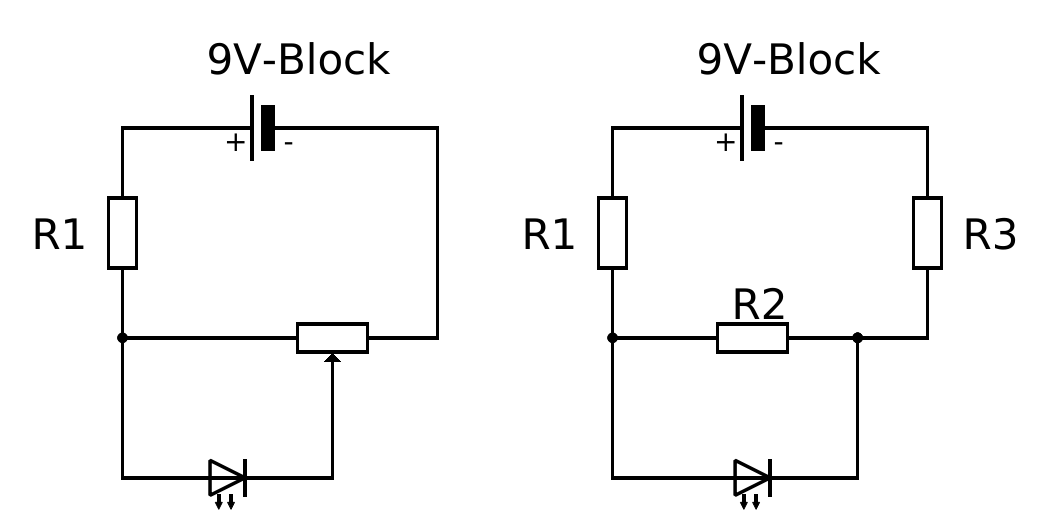
\includegraphics[width=0.6\textwidth]{./Zeichnungen/potentiometer-anwendung.png}
	\caption{Auf der linken Seite ist die Anwendung eines Potentiometers ohne Mikrocontroller dargestellt. Auf der rechten Seite ist der zugehörige Ersatzschaltplan gezeichnet, der zeigt, dass das Potentiometer als Spannungsteiler mit zwei variablen Widerständen $R_2$ und $R_3$ aufgefasst werden kann.}
\end{figure}

\begin{projekt}[Dimmbare Lampe ohne Mikrocontroller]\label{proj:dimmlampeomc}
	\vspace{-0.5\baselineskip}
	\begin{enumerate}[label=\alph*), itemsep=0mm, parsep=0mm]
		\item Erkläre, wie sich die LED verhält, wenn das Potentiometer so gedreht ist, dass gilt:
		\begin{enumerate}[label=(\arabic*), itemsep=0mm, parsep=0mm]
			\item \dots $R_2=\SI{0}{\ohm}, \quad R_3=\SI{10}{\kilo\ohm}$,
			\item \dots $R_2=\SI{10}{\kilo\ohm}, \quad R_3=\SI{0}{\ohm}$.
		\end{enumerate} 
		\item Bevor die Schaltung aufgebaut werden kann, muss die Größe des Vorwiderstands $R_1$ berechnet werden. Der Vorwiderstand muss den Strom auch dann noch klein genug halten, wenn das Potentiometer so gedreht ist, dass gilt: $R_3=\SI{0}{\ohm}$ (und dementsprechend $R_2=\SI{10}{\kilo\ohm}$).
		
		Berechne $R_1$ so, dass die Stromstärke durch die LED maximal $\SI{20}{\milli\ampere}$ beträgt.
		
		\emph{Hinweis:} Die Stromstärke durch $R_2$ kann vernachlässigt werden, sodass $I_{ges}\approx I_{LED} = \SI{20}{\milli\ampere}$ mit $U_{LED}=\SI{2,3}{\volt}$ gilt.
		
		\emph{Begründung:} Wenn $R_1=\SI{0}{\ohm}$ wäre, würde die komplette Spannung an $R_2$ abfallen. Dann gilt: $I_{R_2}=\frac{\SI{9}{\volt}}{\SI{10}{\kilo\ohm}}=\SI{0,9}{\milli\ampere}$. Die Stromstärke durch $R_2$ beträgt also nur etwa 1/20 der Stromstärke durch die LED und wenn $R_1$ größer wird, dann wird die Stromstärke durch $R_2$ sogar noch kleiner. 
		
		\item Baue die Schaltung auf und beobachte das Leuchtverhalten der LED beim Drehen am Potentiometer.
	\end{enumerate}
\end{projekt}

\newpage
Beim Experimentieren mit dem Potentiometer wirst du feststellen, dass man das Potentiometer nicht vollständig zur Seite drehen muss, damit die LED aufhört zu leuchten. Im Experiment zeigt sich, dass eine blaue LED schon bei $R_2=\SI{2,5}{\kilo\ohm}$ und $R_3=\SI{7,5}{\kilo\ohm}$ aufhört zu leuchten. Die Spannung an der LED beträgt dann $U_{L,blau}=\SI{2,3}{\volt}$.

\begin{aufgabe} \emph{Kennlinien von Leuchtdioden}
	\begin{enumerate}[label=\alph*), itemsep=0mm, parsep=0mm]
		\item Baue eine blaue LED in den oben dargestellten Schaltkreis und drehe das Potentiometer so, dass die blaue LED gerade nicht mehr leuchtet. Die Spannung an der blauen LED beträgt dann $U_{L,blau}=\SI{2,3}{\volt}$. Ersetze dann die blaue LED durch eine grüne/gelbe/rote LED. Notiere deine Beobachtungen.
		\item Ordne die Farben der LEDs den rechts abgebildeten Kennlinien von einer blauen, einer grünen, einer gelben und einer roten LED zu. Experimentiere dazu mit dem Potentiometer und den LEDs.
		
		\emph{Hinweis:} Das menschliche Auge ist in der Lage, bereits bei einer Stromstärke von wenigen Mikroampere ein schwaches Leuchten zu erkennen. Im Diagramm ist so eine geringe Stromstärke kaum von $\SI{0}{\milli\ampere}$ zu unterscheiden.
	\end{enumerate}
	
	\begin{figure}[H]
		\centering
		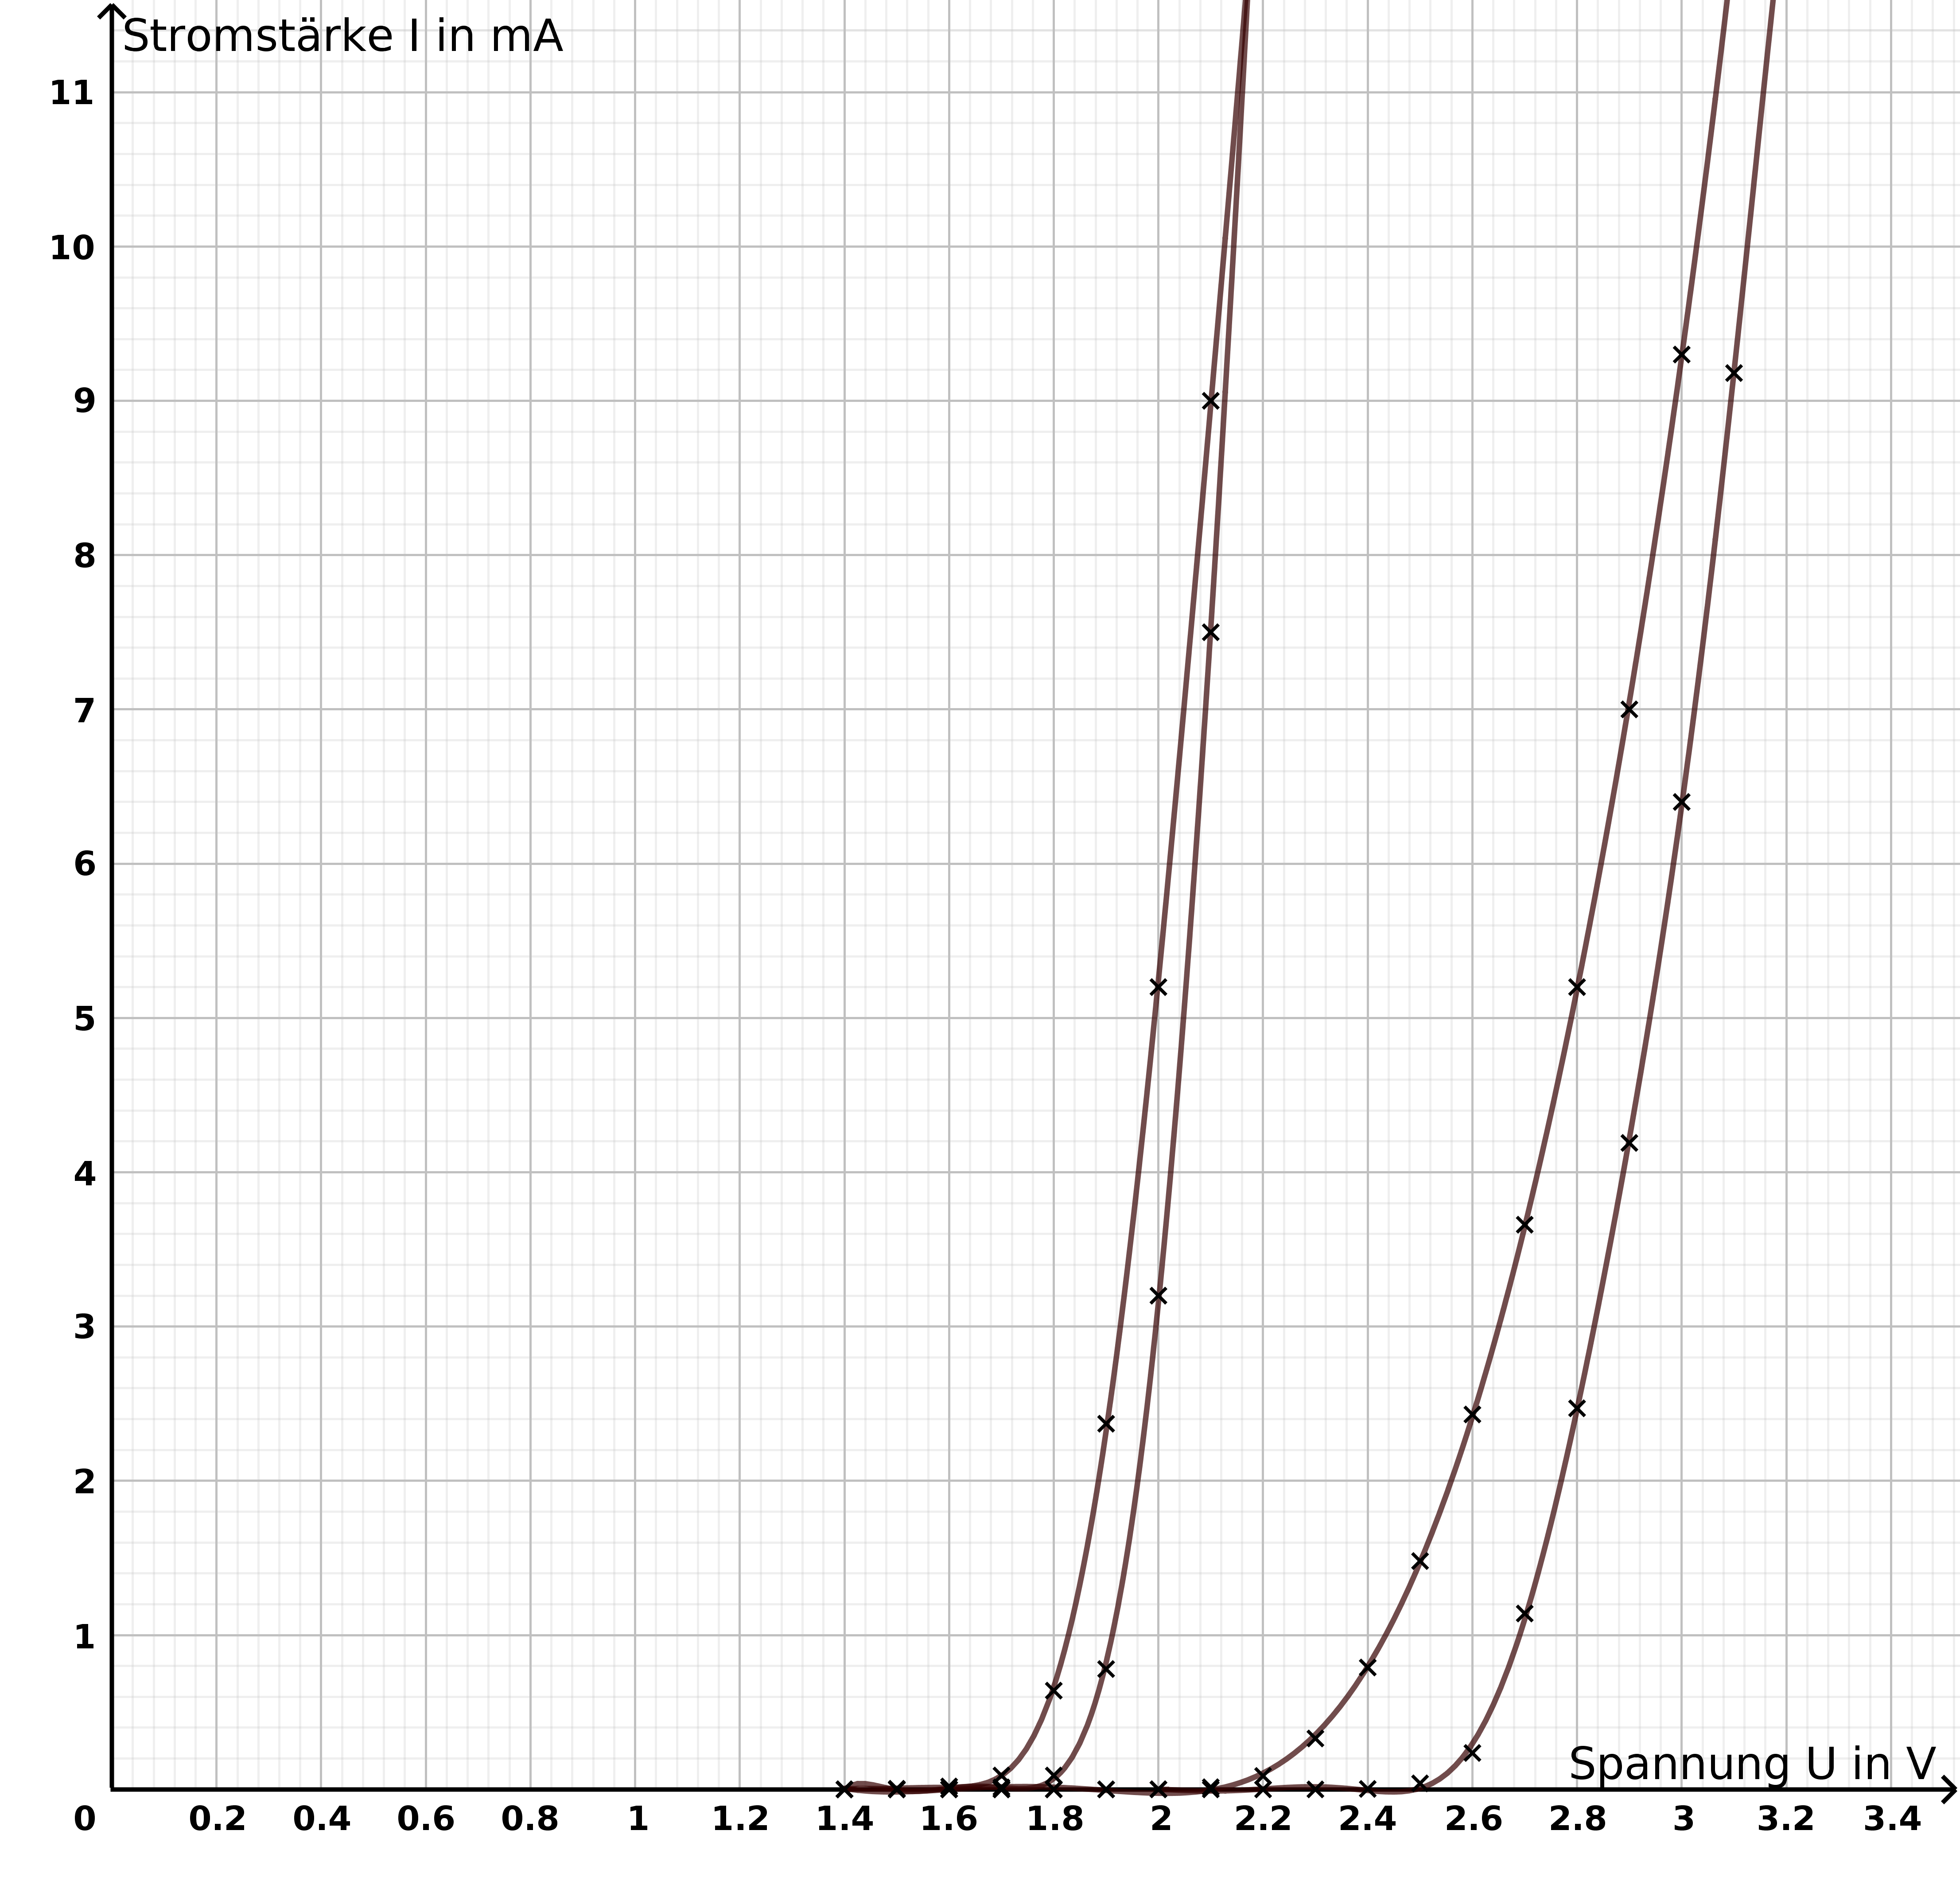
\includegraphics[width=0.85\textwidth]{./Zeichnungen/Diodenkennlinien.png}
		\caption{U-I-Kennlinien einer roten, gelben, grünen und blauen Leuchtdiode.}
	\end{figure}
\end{aufgabe}
\vfill

\section{Helligkeit messen}
\label{sec:helligkeit}

\begin{minipage}{0.84\textwidth}
	Die Helligkeit bestimmt unseren Tages- und Jahresrhythmus: Wenn es dunkel wird, schlafen wir (oder gehen feiern) und wenn es hell wird, stehen wir wieder auf und unternehmen etwas. Es ist daher nur logisch, dass es einige Anwendungen für elektrische Schaltungen gibt, die auf die Helligkeit reagieren.
	
	In einfachen Fällen wird dabei auf einen Fotowiderstand, kurz: LDR (\emph{engl. \textbf{l}ight \textbf{d}ependent \textbf{r}esistor}), zurückgegriffen. Diesen hast du bereits in Abschnitt \ref{sec:seriellermonitor} kennen gelernt: Sein Widerstand wird umso kleiner, je heller es ist.
\end{minipage}
\hfill
\begin{minipage}{0.14\textwidth}
	\begin{figure}[H]
		\centering
		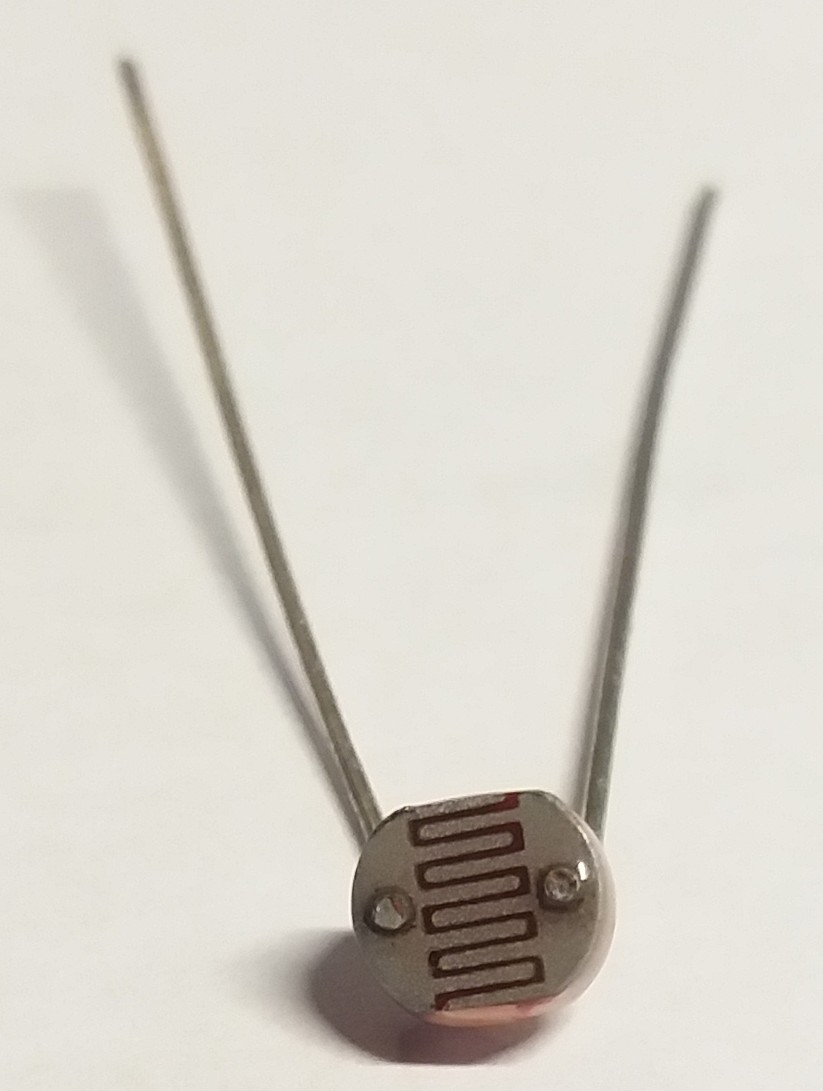
\includegraphics[width=0.9\textwidth]{./pics/ldr.jpg}
		\caption{Ein LDR.}
	\end{figure}
\end{minipage}

\begin{ziel}
	\textbf{Frage:} Wie bestimmt man mit Hilfe von Analogwerten die Helligkeit?
\end{ziel}

\medskip
\begin{minipage}{0.73\textwidth}
	\begin{aufgabe} \emph{LDR revisited}
		\begin{enumerate}[label=\alph*), itemsep=0ex, parsep=0ex]
			\item Die Abbildung rechts zeigt noch einmal, wie der LDR in Abschnitt \ref{sec:seriellermonitor} am Arduino angeschlossen wurde. Erläutere, was im Spannungsteiler passiert, wenn die Helligkeit erhöht wird. Halte dich dabei an folgende Schritte:
			
			Widerstand des LDR $\rightarrow$ Spannung am LDR $\rightarrow$ Spannung am Festwiderstand $\rightarrow$ Analogwert in A0.
			\item Unten ist abgebildet, wie die Anweisung \texttt{gib Licht \% Lichtsensor LDR} intern umgesetzt wird. Begründe, dass diese Angabe als Angabe für die physikalische Größe Helligkeit ungeeignet ist.
			% eigentlich wird die Spannung gemessen und Spannung und Helligkeit sind nicht proportional; zudem: keine Einheit - Prozent von was? - keine absolute Bezugsgröße / wieso sollen 100\% alles sein und was ist mit noch größeren Helligkeiten?
		\end{enumerate}
	\end{aufgabe}
\end{minipage}
\hfill
\begin{minipage}{0.25\textwidth}
	\centering
	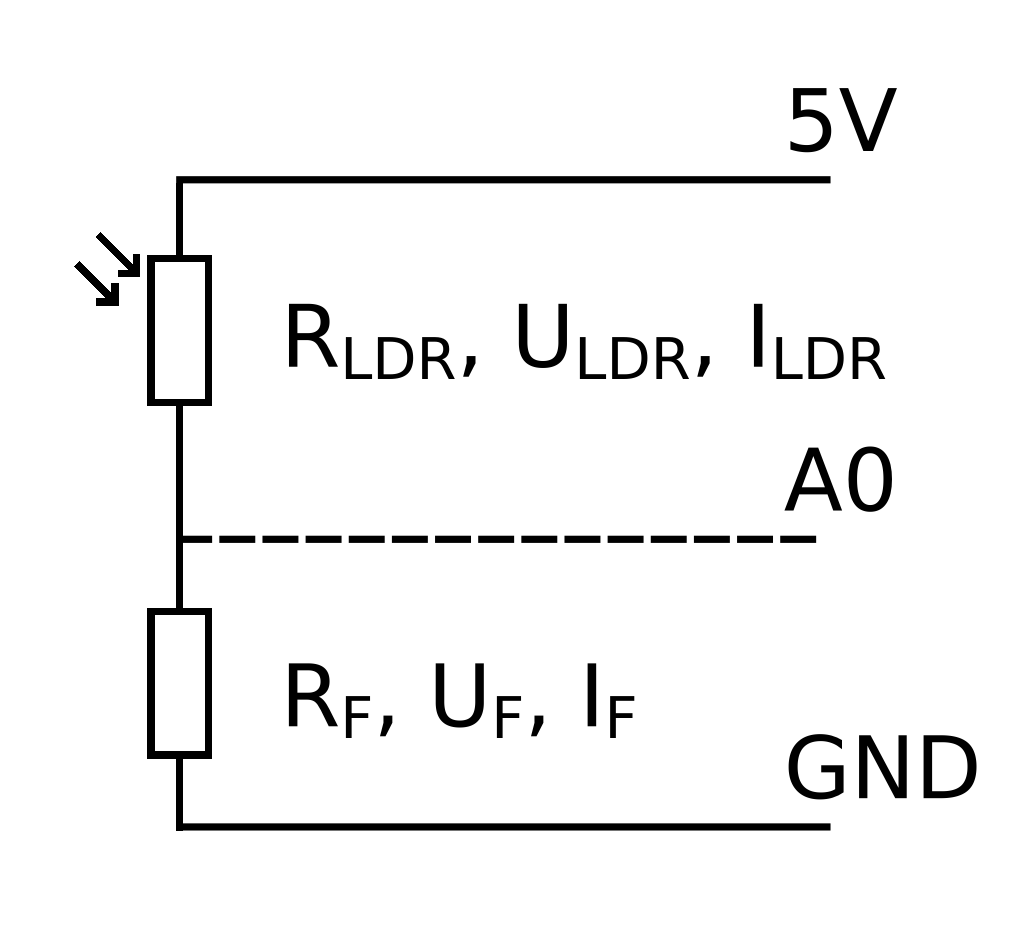
\includegraphics[width=\textwidth]{./Zeichnungen/spannungsteiler-ldr-beschriftet-2.png}
\end{minipage}

\begin{figure}[H]
	\centering
	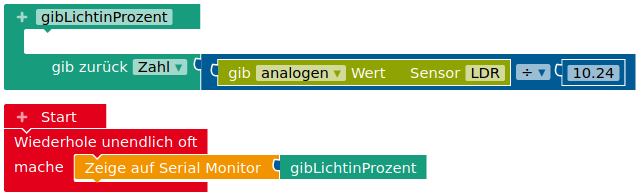
\includegraphics[width=0.7\linewidth]{./pics/gibLichtInProzent-Funktion.png}
	\caption{Die Anweisung \texttt{Gib Licht \% Lichtsensor LDR} als selbst definierte Funktion.}
\end{figure}

\begin{minipage}{0.73\textwidth}
	\begin{aufgabe}\emph{Der LDR im Spannungsteiler}
%		\vspace{-0.3\baselineskip}
		\begin{enumerate}[label=\alph*), itemsep=0ex, parsep=0mm]
			\item Um nicht ständig umdenken zu müssen, soll der Spannungsteiler von LDR und Festwiderstand $R_F=\SI{10}{\kilo\ohm}$ nun wie rechts abgebildet aufgebaut werden. Lasse dir die Spannung am LDR auf dem seriellen Monitor ausgeben.
			\item Erläutere wiederum, was im Spannungsteiler passiert, wenn die Helligkeit erhöht wird.
		\end{enumerate}
	\end{aufgabe}
\end{minipage}
\hfill
\begin{minipage}{0.25\textwidth}
	\centering
	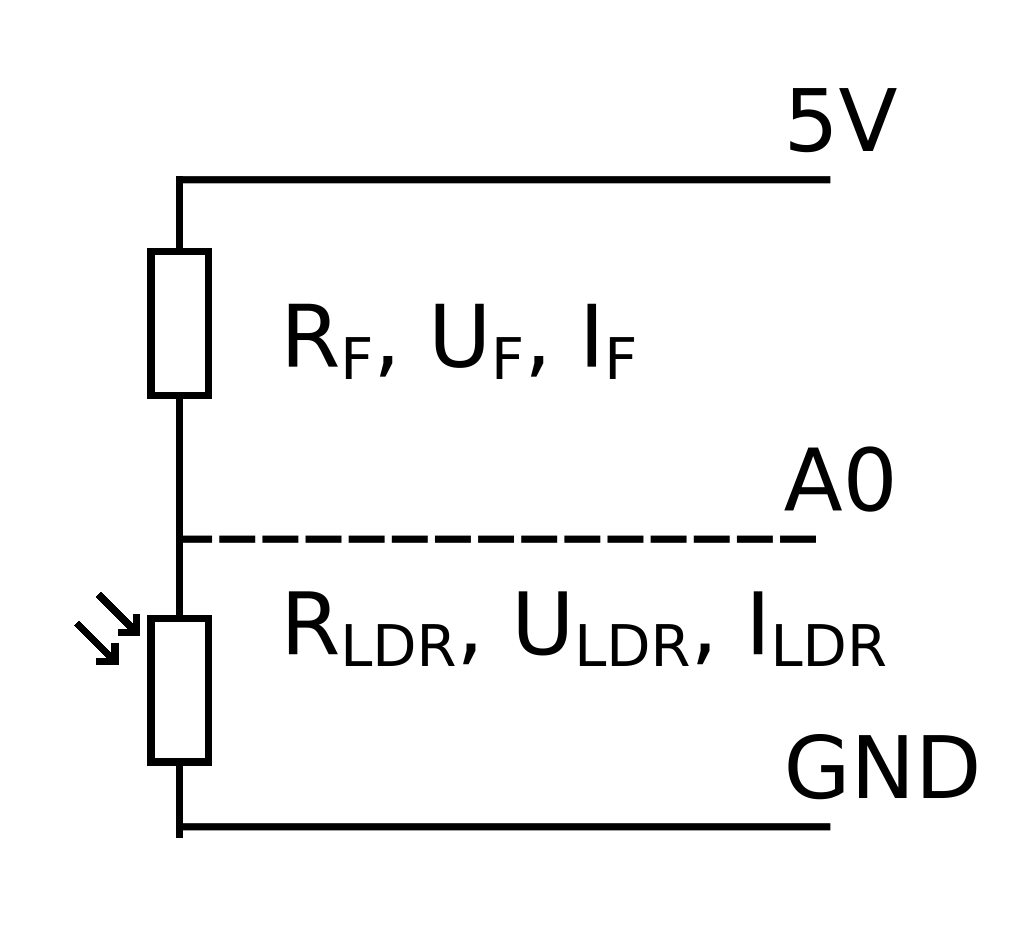
\includegraphics[width=\textwidth]{./Zeichnungen/spannungsteiler-ldr-beschriftet.png}
\end{minipage}

Die Änderung der Spannung resultiert aus der Änderung des Widerstands des LDR. Um einen Eindruck vom Wertebereich des Widerstands eines LDR zu bekommen, soll dieser nun berechnet werden. Anschließend lässt sich aus dem Widerstand des LDR auch die Helligkeit berechnen.
\marginpar{%
	\textattachfile[description={Folie zu Kap. \thechapter, Spannungsteilerformel}]{./Auftraege/kap4-spannungsteiler.pdf}{%
		\footnotesize\folie Folie%
	}%
	\footnotesize%
	%	\folie \href{run:./Auftraege/kap3-auftrag-potential.pdf}{Folie}%
	\\öffnen
}

\begin{aufgabe} \emph{Genaue Analyse des Spannungsteilers}
	\vspace{-0.3\baselineskip}
	\begin{enumerate}[label=\alph*), itemsep=0ex, parsep=0mm]
		\item Leite eine Formel für den Spannungsteiler her, mit der du den Widerstand $R_{LDR}$ des LDR mithilfe der Spannung $U_{LDR}$ am LDR, dem Festwiderstand $R_F$ und der Spannung $U_F$ am Festwiderstand berechnen kannst.
		
		Tipp: Betrachte zuerst die Stromstärken $I_F$ und $I_{LDR}$ durch den Festwiderstand und den LDR. Durch das Sensorkabel fließt (näherungsweise) kein Strom.
		\item Berechne, welchen Widerstand der LDR hat, wenn er komplett abgedunkelt ist und wenn er mit einer Smartphone-Taschenlampe bestrahlt wird.
	\end{enumerate}
\end{aufgabe}

\begin{zsfg}{Der Spannungsteiler}
	
	\begin{wrapfigure}{r}{0.25\textwidth}
		\centering
		\vspace{-0.5\baselineskip}
		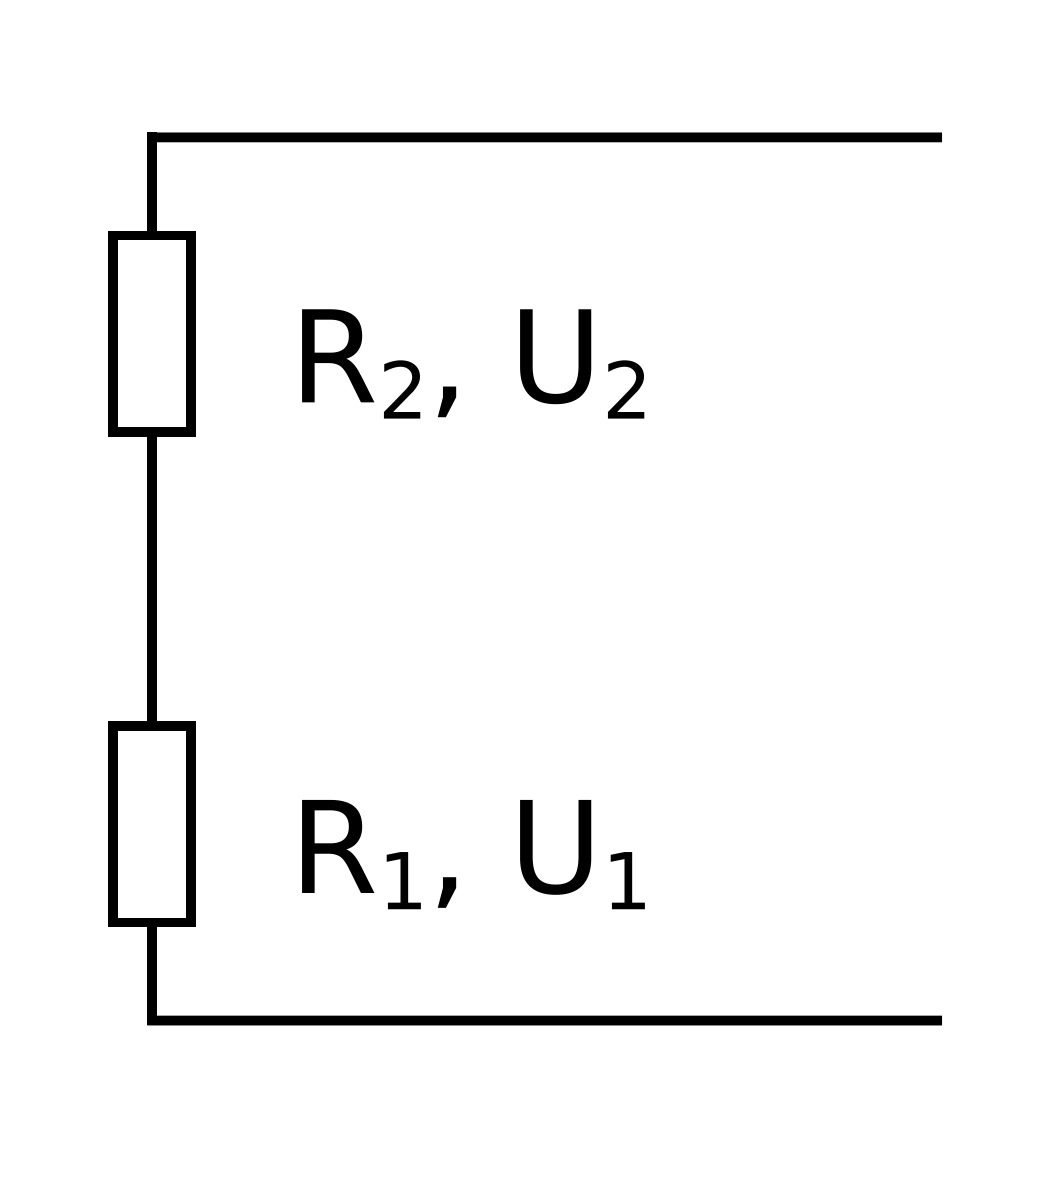
\includegraphics[width=0.8\linewidth]{./Zeichnungen/spannungsteiler.png}
	\end{wrapfigure}
	Der Spannungsteiler ist ein häufig verwendeter Teil einer Schaltung, in dem zwei Widerstände in Reihe geschaltet sind. Dadurch teilt sich die insgesamt anliegende Spannung auf die beiden Widerstände entsprechend ihrer jeweiligen Größe auf. Dabei gilt:
	\begin{equation*}
		\frac{U_1}{R_1} = \frac{U_2}{R_2} = \frac{U_{ges}}{R_{ges}}.
	\end{equation*}
\end{zsfg}

%%Infokasten: LDR als elektronisches Bauteil, das seinen Widerstand in Abhängigkeit der Helligkeit ändert (mit Bild und Schaltsymbol)
%\begin{zsfg}{Fotowiderstand}
%	\begin{minipage}{0.7\textwidth}
%		Ein \textbf{Fotowiderstand}, kurz: \textbf{LDR} (\emph{engl. \textbf{l}ight \textbf{d}ependent \textbf{r}esistor}), ist ein lichtabhängiger Widerstand. Wenn es dunkel wird, wird der elektrische Widerstand des LDR größer; wenn es hell wird, wird der elektrische Widerstand des LDR kleiner.
%	\end{minipage}
%	\hfill
%	\begin{minipage}{0.28\textwidth}
%		\begin{minipage}{0.48\textwidth}
%			\centering
%			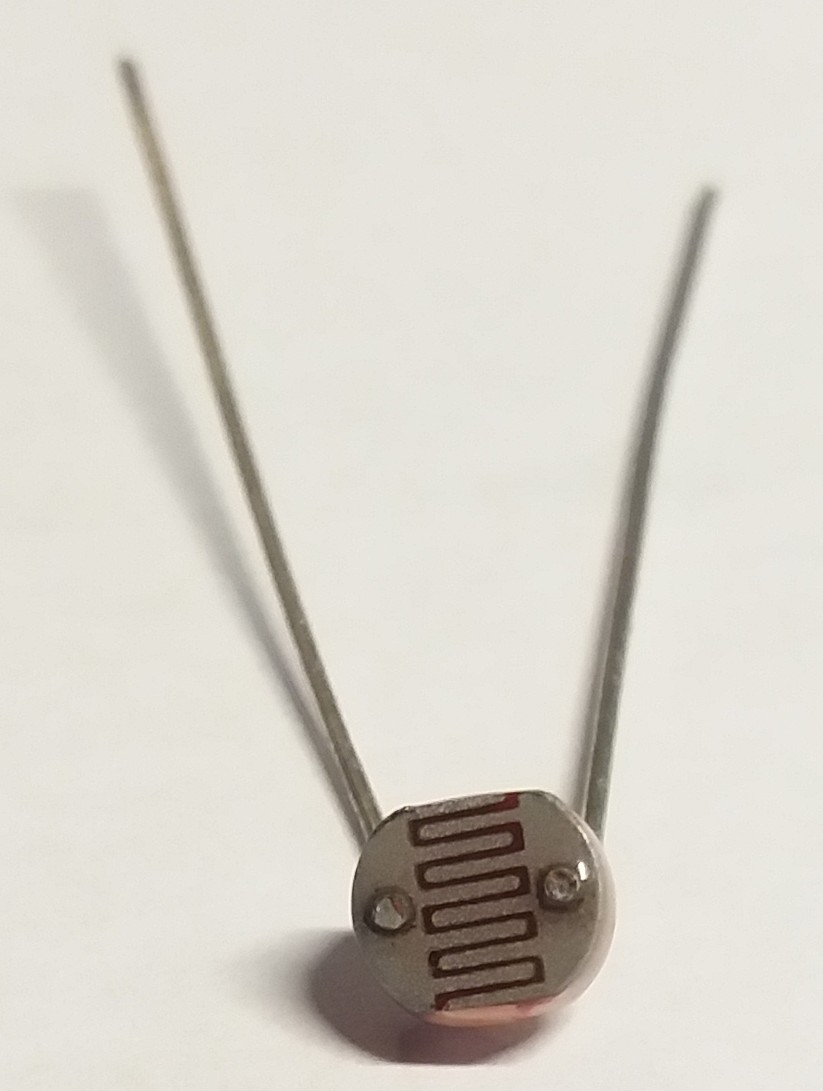
\includegraphics[width=0.9\textwidth]{./pics/ldr.jpg}
%		\end{minipage}
%		\hfill
%		\begin{minipage}{0.48\textwidth}
%			\centering
%			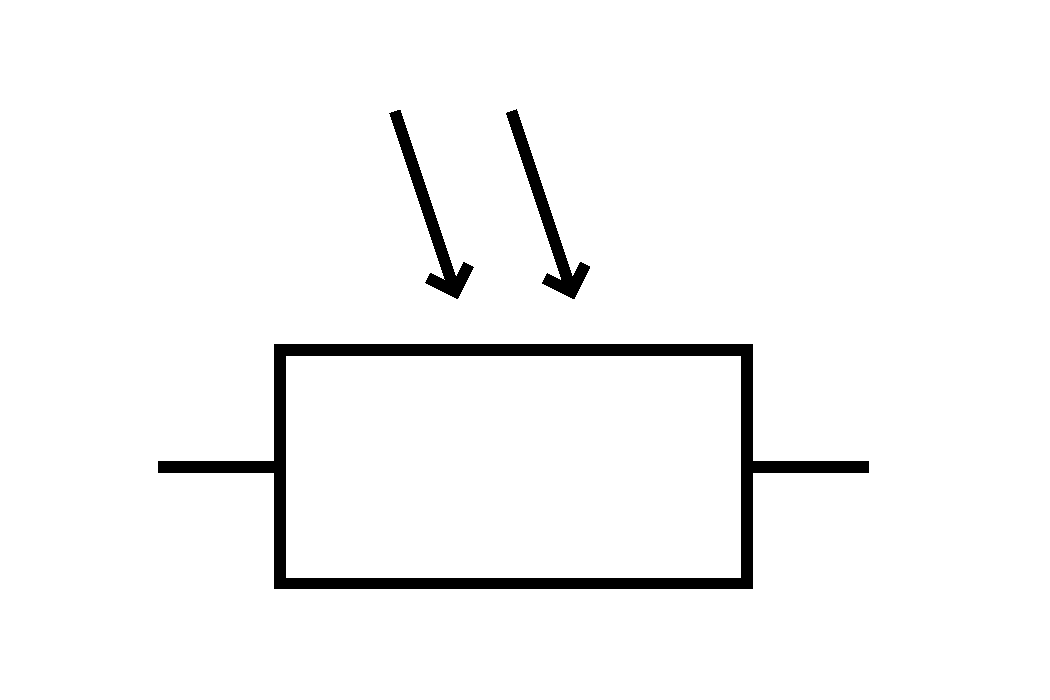
\includegraphics[width=\textwidth]{./pics/ldr-schaltsymbol.png}
%		\end{minipage}
%	\end{minipage}
%	%	\bigskip
%	%	\emph{Kurze Hintergrundinformation:}
%	%	
%	%	Der Fotowiderstand besteht aus einem Halbleitermaterial, in dem die Elektronen wie üblich an den Atomkern gebunden sind. Bei Halbleitern reicht jedoch schon relativ wenig Energie, um einige Elektronen so weit aus ihrer Bindung zu lösen, dass sie zum elektrischen Strom beitragen. Diese Energiezufuhr stammt von dem Licht, das auf den LDR fällt.
%\end{zsfg}
%%TODO: Hintergrundinfo ausführlicher - Bändermodell

\bigskip
Um den funktionalen Zusammenhang zwischen Widerstand des LDR und Umgebungshelligkeit herauszufinden, gibt es drei Möglichkeiten:
\begin{itemize}
	\item Theoretische Herleitung: Die Herleitung des Zusammenhangs mit Hilfe von anderen physikalischen Gesetzen und Annahmen führt an dieser Stelle zu weit,
	\item Experimentelle Ermittlung: Dazu müssten einige Widerstandswerte bei vorgegebener Helligkeit gemessen werden, jedoch ist es schwierig, eine vorgegebene Helligkeit genau herzustellen,
	\item Blick ins Datenblatt: Zu jedem Bauteil gibt es ein Datenblatt, in dem die zugehörigen Kennzahlen und Zusammenhänge dargestellt sind - hier können die Ergebnisse von Laborexperimenten eingesehen werden.
\end{itemize}
\bigskip

\begin{aufgabe} \emph{Datenblatt lesen}
	
	Suche im \href{https://components101.com/sites/default/files/component_datasheet/LDR%20Datasheet.pdf}{Datenblatt des LDR}
	den Graphen, der den Zusammenhang von Helligkeit in der Einheit Lux und Widerstand des LDR in der Einheit $\SI{}{\kilo\ohm}$ abbildet. Entnimm dem Graphen fünf zusammengehörige Werte von Helligkeit und Widerstand und halte diese tabellarisch fest.
	
	\smallskip
	\begin{minipage}{0.78\textwidth}
		\emph{Achtung:} Die Achsen im Graphen sind logarithmisch skaliert. Das bedeutet, dass die Werte an den Achsen nicht gleichmäßig zunehmen, sondern exponentiell (von 0,1 zu 1 zu 10 zu 100 zu 1000). Diese Skalierung ermöglicht erst das Ablesen der Werte, aber es muss berücksichtigt werden, dass die Werte nur sehr ungenau abzulesen sind.
	\end{minipage}
	\hfill
	\begin{minipage}{0.2\textwidth}
		\begin{tikzpicture}
		\draw [->] (-0.2,0) -- (2.2,0);
		\draw [->] (0,-0.2) -- (0,2.2);
		\draw (0.5,0.1) -- ++(0,-0.2) node [below] {\tiny 0.1};
		\draw (1,0.1) -- ++(0,-0.2) node [below] {\tiny 1};
		\draw (1.5,0.1) -- ++(0,-0.2) node [below] {\tiny 10};
		\draw (2,0.1) -- ++(0,-0.2) node [below] {\tiny 100};
		\draw (0.1,0.5) -- ++(-0.2,0) node [left] {\tiny 0.1};
		\draw (0.1,1) -- ++(-0.2,0) node [left] {\tiny 1};
		\draw (0.1,1.5) -- ++(-0.2,0) node [left] {\tiny 10};
		\draw (0.1,2) -- ++(-0.2,0) node [left] {\tiny 100};
		\end{tikzpicture}
	\end{minipage}
		
	\smallskip
	\textit{\small Das verlinkte Datenblatt ist evtl. nicht das korrekte Datenblatt zu dem LDR. Da die Bauteilnummer bei dem verwendeten Starter Kit nicht angegeben wird, ist eine Zuordnung leider nicht mehr möglich.}
\end{aufgabe}

\begin{aufgabe} \emph{Regression durchführen}
	
	Unabhängig davon, ob man die Daten aus einem Experiment oder dem Datenblatt gewonnen hat, lässt sich nun eine Regression durchführen, um den allgemeinen Zusammenhang zwischen Widerstand des LDR und Helligkeit herauszufinden.
	
	Führe mit den ermittelten Werten eine Regression durch, indem du die unten abgebildete Anleitung befolgst. Bestimme mit der erhaltenen Funktion die Umgebungshelligkeit im Raum sowie die Helligkeit deiner Smartphone-Taschenlampe auf niedrigster und höchster Stufe.
\end{aufgabe}

%\restoregeometry
%\onehalfspacing

\newpage
\begin{zsfg}{Eine Regression durchführen}
	
	Beim Durchführen einer Regression wird diejenige Funktion(sgleichung) ermittelt, die am besten zu den gegebenen Daten passt. Die Art der Funktion muss jedoch vom Anwender sinnvoll festgelegt werden.
\end{zsfg}	
\begin{zsfg}{Regression mit TI Nspire}
	
	\smallskip
	\begin{minipage}[c][4.5cm][t]{0.48\textwidth}
		\textbf{1.} Erstelle ein neues Dokument mit einer Seite \enquote{Lists \& Spreadsheet}. Benenne eine Spalte als \texttt{rw} (Werte für R, also der Widerstand) und eine Spalte als \texttt{hw} (Werte für die Helligkeit). Ergänze die Werte.
	\end{minipage}
	\hfill
	\begin{minipage}[c][4.5cm][t]{0.48\textwidth}
		\centering
		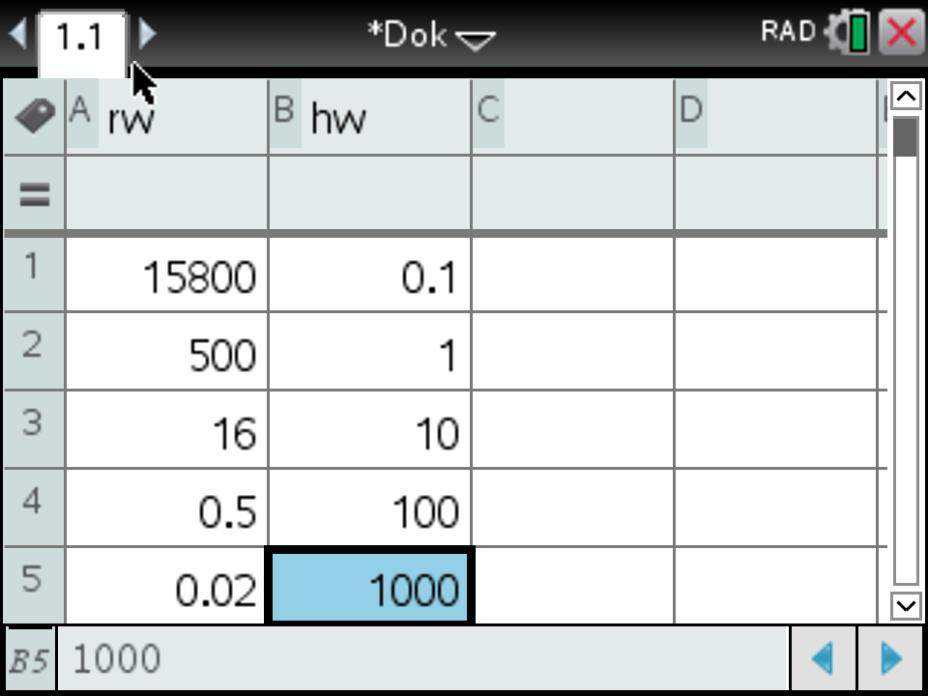
\includegraphics[width=0.8\textwidth]{./pics/RegressionLDR-TI-1.jpg}
	\end{minipage}
	
	
	\begin{minipage}[c][4.5cm][t]{0.48\textwidth}
		\textbf{2.} Füge eine neue Seite \enquote{Data \& Statistics} hinzu (mit \texttt{ctrl} $\rightarrow$ \texttt{+page}). Da wir die Helligkeit in Abhängigkeit vom Widerstand berechnen wollen, kommt der Widerstand auf die Rechtsachse und die Helligkeit auf die Hochachse.
	\end{minipage}
	\hfill
	\begin{minipage}[c][4.5cm][t]{0.48\textwidth}
		\centering
		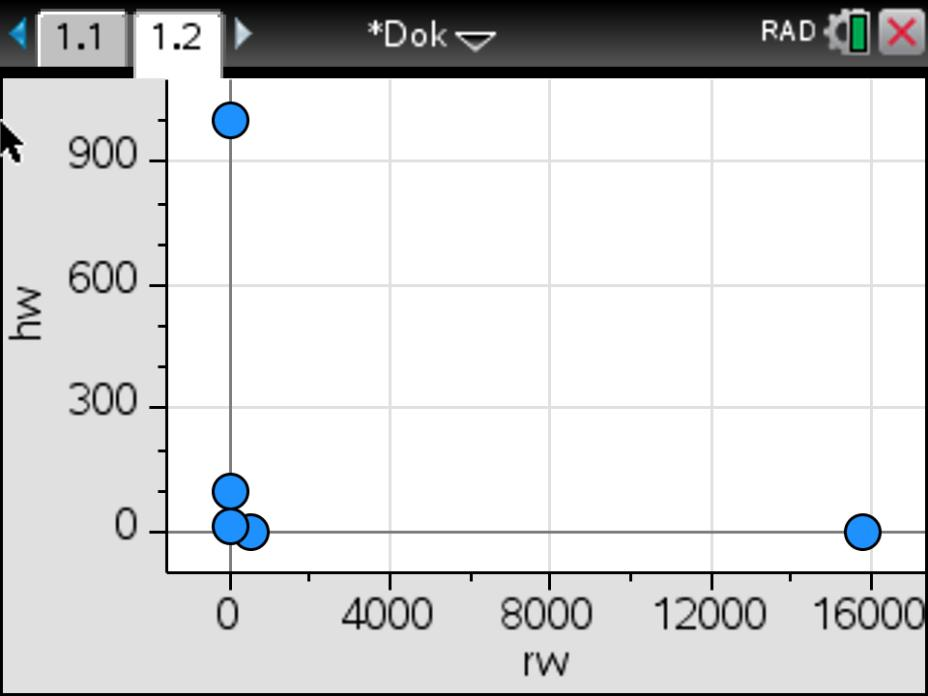
\includegraphics[width=0.8\textwidth]{./pics/RegressionLDR-TI-2.jpg}
	\end{minipage}
	
	\begin{minipage}[c][6cm][t]{0.48\textwidth}
		\textbf{3.} Führe eine Regression durch (\texttt{menu} $\rightarrow$ \texttt{4: Analysieren} $\rightarrow$ \texttt{6: Regression}). Welche Funktionsklasse könnte zu der Verteilung der Werte passen? Falls die ausprobierte Funktionsklasse nicht zu den Werten passt, mache die Regression rückgängig (\texttt{ctrl} $\rightarrow$ \texttt{esc}) und probiere eine andere Funktionsklasse.
		
		\emph{Achtung:} Durch die geringe Auflösung des Taschenrechners können auch passende Funktionen ggf. falsch aussehen.
	\end{minipage}
	\hfill
	\begin{minipage}[c][6cm][t]{0.48\textwidth}
		\centering
		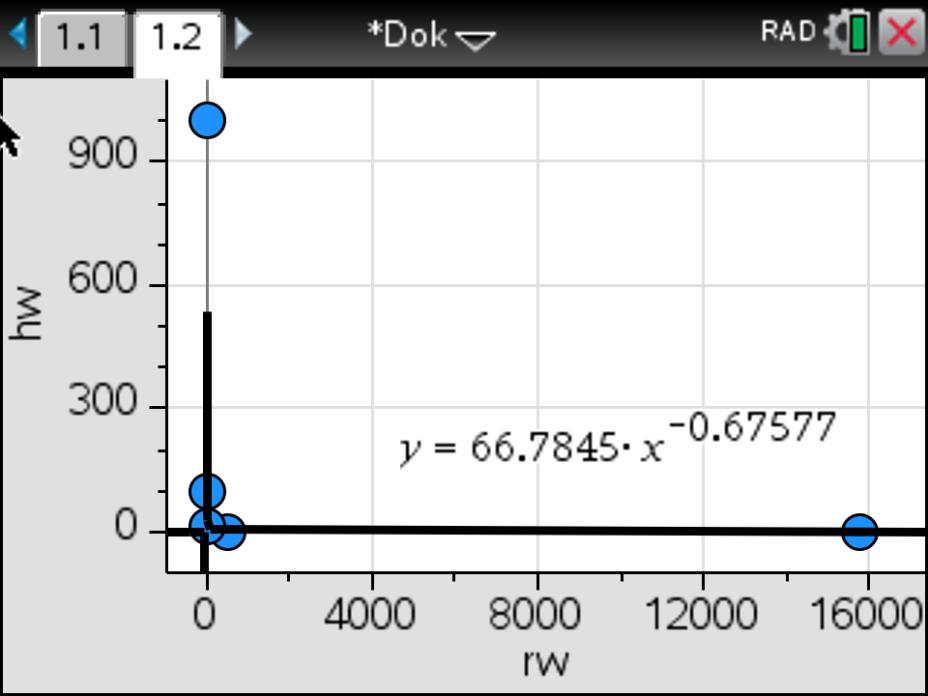
\includegraphics[width=0.8\textwidth]{./pics/RegressionLDR-TI-3.jpg}
	\end{minipage}
	
	\bigskip
	\begin{minipage}[c][3cm][t]{0.48\textwidth}
		\textbf{4.} Übersetze die Funktionsgleichung in den physikalischen Zusammenhang. Für den Widerstand ist das Formelzeichen $R$ festgelegt. Für die Helligkeit wählen wir an dieser Stelle $H$.
	\end{minipage}
	\hfill
	\begin{minipage}[c][3cm][t]{0.48\textwidth}
		\centering
		\vspace{-\baselineskip}
		\begin{align*}
			y &= 66,78 \cdot x^{-0,66} \\
			\downarrow & \hspace{1.6cm}\downarrow \\
			H &= 66,78 \cdot R^{-0,66} \\
			R &\text{ in } \SI{}{\kilo\ohm}, ~ H \text{ in Lux} 
		\end{align*}
	\end{minipage}
\end{zsfg}
\vfill

\begin{zsfg}{Regression mit Geogebra Classic}
	
	\smallskip
	\begin{minipage}[c][4cm][t]{0.48\textwidth}
		\textbf{1.} Starte Geogebra Classic und wähle als Perspektive die Tabellenkalkulation. Übertrage die Daten in die Tabellenkalkulation.
	\end{minipage}
	\hfill
	\begin{minipage}[c][4cm][t]{0.48\textwidth}
		\centering
		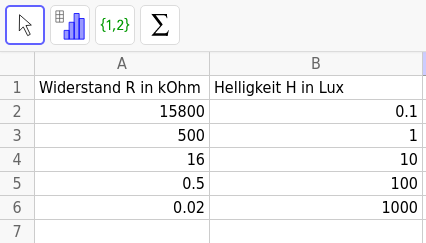
\includegraphics[width=0.8\textwidth]{./pics/RegressionLDR-GGB-1.png}
	\end{minipage}
	
	
	\begin{minipage}[c][4cm][t]{0.48\textwidth}
		\textbf{2.}  Markiere alle Daten und wähle das Werkzeug \texttt{Analyse zweier Variablen}. Die Daten aus Spalte A werden automatisch als x-Koordinate gewählt, die aus Spalte B als y-Koordinate. Bei Bedarf kann dies mit $X \rightleftarrows Y$ vertauscht werden (oben rechts).
	\end{minipage}
	\hfill
	\begin{minipage}[c][4cm][t]{0.48\textwidth}
		\centering
		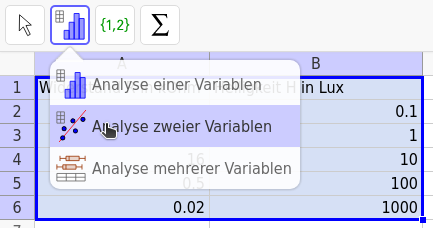
\includegraphics[width=0.8\textwidth]{./pics/RegressionLDR-GGB-2.png}
	\end{minipage}
	
	\begin{minipage}[c][7.5cm][t]{0.48\textwidth}
		\textbf{3.} Führe eine Regression durch, indem du unten links ein passendes Regressionsmodell wählst. Welche Funktionsklasse könnte zu der Verteilung der Werte passen? Falls die ausprobierte Funktionsklasse nicht zu den Werten passt, probiere eine andere Funktionsklasse.
		
		\emph{Hinweis:} Die Anzahl der Nachkommastellen lässt sich in den Einstellungen unter \enquote{Runden} ändern.
	\end{minipage}
	\hfill
	\begin{minipage}[c][7.5cm][t]{0.48\textwidth}
		\centering
		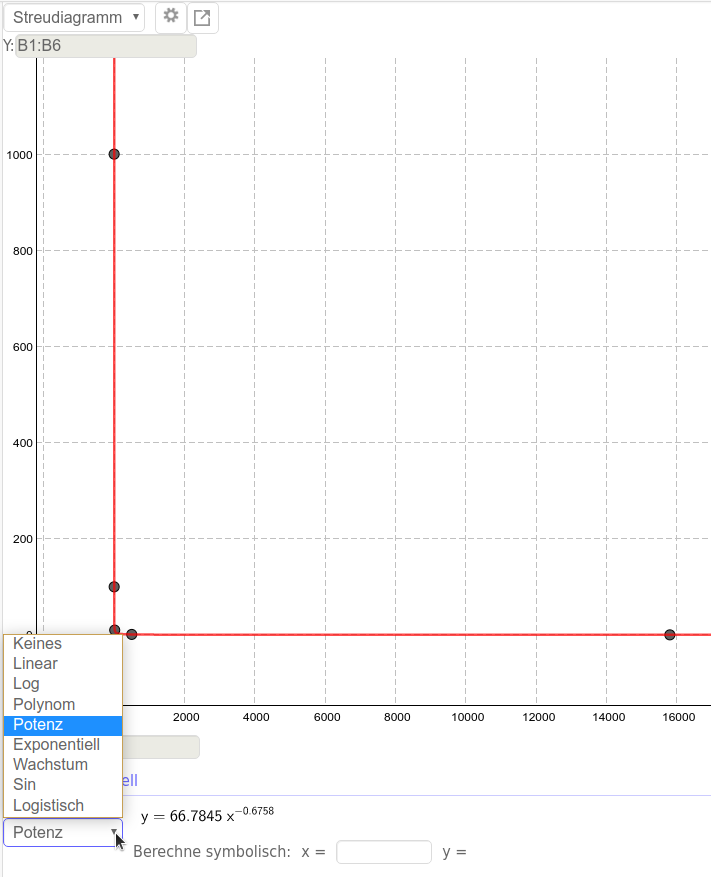
\includegraphics[width=0.8\textwidth]{./pics/RegressionLDR-GGB-3.png}
	\end{minipage}
	
	\begin{minipage}[c][3cm][t]{0.48\textwidth}
		\textbf{4.} Übersetze die Funktionsgleichung in den physikalischen Zusammenhang. Für den Widerstand ist das Formelzeichen $R$ festgelegt. Für die Helligkeit wählen wir an dieser Stelle $H$.
	\end{minipage}
	\hfill
	\begin{minipage}[c][3cm][t]{0.48\textwidth}
		\centering
		\vspace{-\baselineskip}
		\begin{align*}
			y &= 66,78 \cdot x^{-0,66} \\
			\downarrow & \hspace{1.6cm}\downarrow \\
			H &= 66,78 \cdot R^{-0,66} \\
			R &\text{ in } \SI{}{\kilo\ohm}, ~ H \text{ in Lux} 
		\end{align*}
	\end{minipage}
\end{zsfg}
\vfill
	
%Exkurs/Hintergrund: Wieso ändert sich der Widerstand des LDR, wenn Licht auf ihn trifft? -> Erklärung im Energiebändermodell
	
% TODO: Lichttheremin als Projekt?
	

\newpage
\section{Temperatur messen}
\label{sec:ntc}

\begin{wrapfigure}{r}{0.15\textwidth}
	\centering
	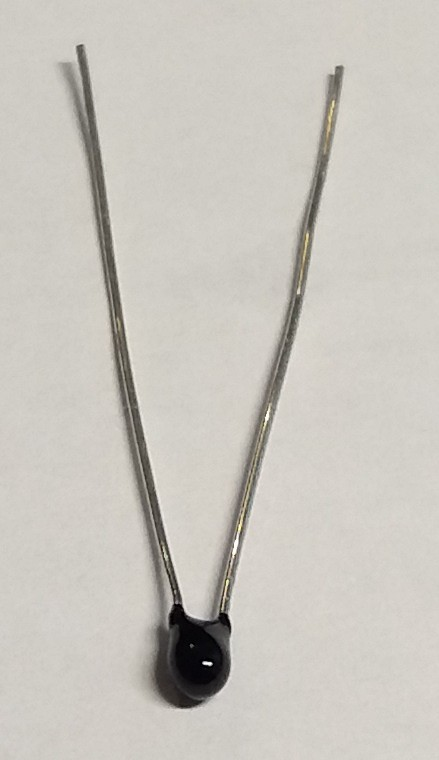
\includegraphics[width=0.1\textwidth]{./pics/ntc.jpg}
	\caption{Ein NTC.}
\end{wrapfigure}
Nicht nur die Helligkeit beeinflusst unseren Alltag, sondern auch die Temperatur. Ganz allgemein ist die Temperatur eine wichtige Größe, die bei vielen Anwendungen eine Rolle spielt und daher erfasst und automatisiert in die Anwendung einfließen sollte: Thermostate regeln die Temperatur im Raum, Wetterstationen geben die Temperatur an und 3D-Drucker regeln die Temperatur der Düse auf eine festgelegte Temperatur, damit der Kunststoff flüssig wird, aber immer noch zäh genug bleibt, um die Figur zu bilden. Häufig wird dabei ein Heißleiter (kurz: NTC, von engl. \emph{negative temperature coefficient}) verwendet - ein elektrischer Widerstand, der auf die Temperatur reagiert.

\begin{ziel}
	\textbf{Frage:} Wie verwendet man einen NTC am Arduino?
\end{ziel}

\begin{aufgabe} \emph{Erste Experimente mit dem NTC}
	\begin{enumerate}[label=\alph*), itemsep=0ex,parsep=0ex]
		\item Baue mithilfe eines Festwiderstands $R_F=\SI{10}{\kilo\ohm}$ und dem NTC einen Spannungsteiler und lies die Spannung am NTC in A0 aus (genau wie beim LDR).
		
		Erwärme den NTC, indem du ihn zwischen Daumen und Zeigerfinger hälst. Beschreibe, wie sich die Spannung am NTC ändert, wenn dieser wärmer wird.
		\item Begründe, dass auch hier gilt:
		\begin{equation*}
			\frac{R_{NTC}}{R_{F}} = \frac{U_{NTC}}{U_{F}}.
		\end{equation*}
		
		Begründe anhand der Formel, wie sich der Widerstand am NTC ändert, wenn dieser wärmer wird.
	\end{enumerate}
\end{aufgabe}

\emph{Hinweis:} Der NTC wird wieder als analoger Sensor konfiguriert. Es handelt sich \emph{nicht} um den Temperatursensor TMP36, der nach einem anderen Prinzip arbeitet.

\medskip
\begin{projekt}[Digitales Thermometer]\label{proj:thermometer}
	\begin{minipage}{0.58\textwidth}
		Baue ein digitales Thermometer, das die Lufttemperatur im Raum auf dem seriellen Monitor anzeigt!
		
		\bigskip
		Führe dazu mithilfe des rechts abgebildeten Ausschnitts \href{https://pdf1.alldatasheet.com/datasheet-pdf/view/509832/EPCOS/G1541.html}{aus einem Datenblatt} eine Regression durch.
		
		\bigskip
		\textit{\small Das verlinkte Datenblatt ist evtl. nicht das korrekte Datenblatt zu dem NTC. Da die Bauteilnummer bei dem verwendeten Starter Kit nicht angegeben wird, ist eine Zuordnung leider nicht mehr möglich.}
		
		\vspace{\baselineskip}
	\end{minipage}
	\hfill
	\begin{minipage}{0.38\textwidth}
		\begin{tcolorbox}[sharp corners]
			R/T No. \textbf{7003}
			
			Widerstand bei $\ang{25}$: 
			
			$R_{25}=\SI{10}{\kilo\ohm}$.\\			
			
			\begin{tabular}{l | l | l}
				T (C) & $R_T/R_{25}$ & (\%/K) \\ \hline
				5.0 & 2.3311 & 4.5 \\ \hline
				10.0 & 1.8684 & 4.4  \\ \hline
				15.0 & 1.5075 &  4.2 \\ \hline
				20.0 & 1.224 & 4.1 \\ \hline
				25.0 & 1.0000 & 4.0 \\ \hline
				30.0 & 0.82176 & 3.9 \\ \hline
			\end{tabular}
		\end{tcolorbox}
	\end{minipage}
\end{projekt}

\begin{zsfg}{Heißleiter}
	\begin{minipage}{0.7\textwidth}
		Ein \textbf{Heißleiter}, kurz: \textbf{NTC} (\emph{engl. \textbf{n}egative \textbf{t}emperature \textbf{c}oefficient}), ist ein temperaturabhängiger Widerstand. Wenn es wärmer wird, wird der elektrische Widerstand des NTC kleiner; wenn es kälter wird, wird der elektrische Widerstand des NTC größer.
	\end{minipage}
	\hfill
	\begin{minipage}{0.28\textwidth}
		\begin{minipage}{0.48\textwidth}
			\centering
			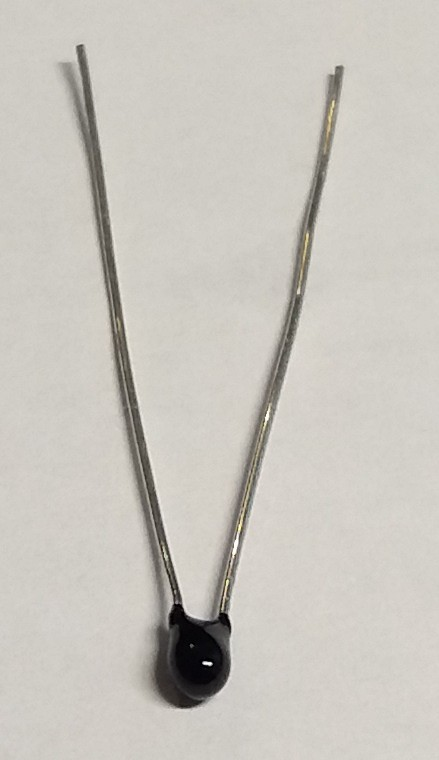
\includegraphics[width=0.9\textwidth, height=2cm]{./pics/ntc.jpg}
		\end{minipage}
		\hfill
		\begin{minipage}{0.48\textwidth}
			\centering
			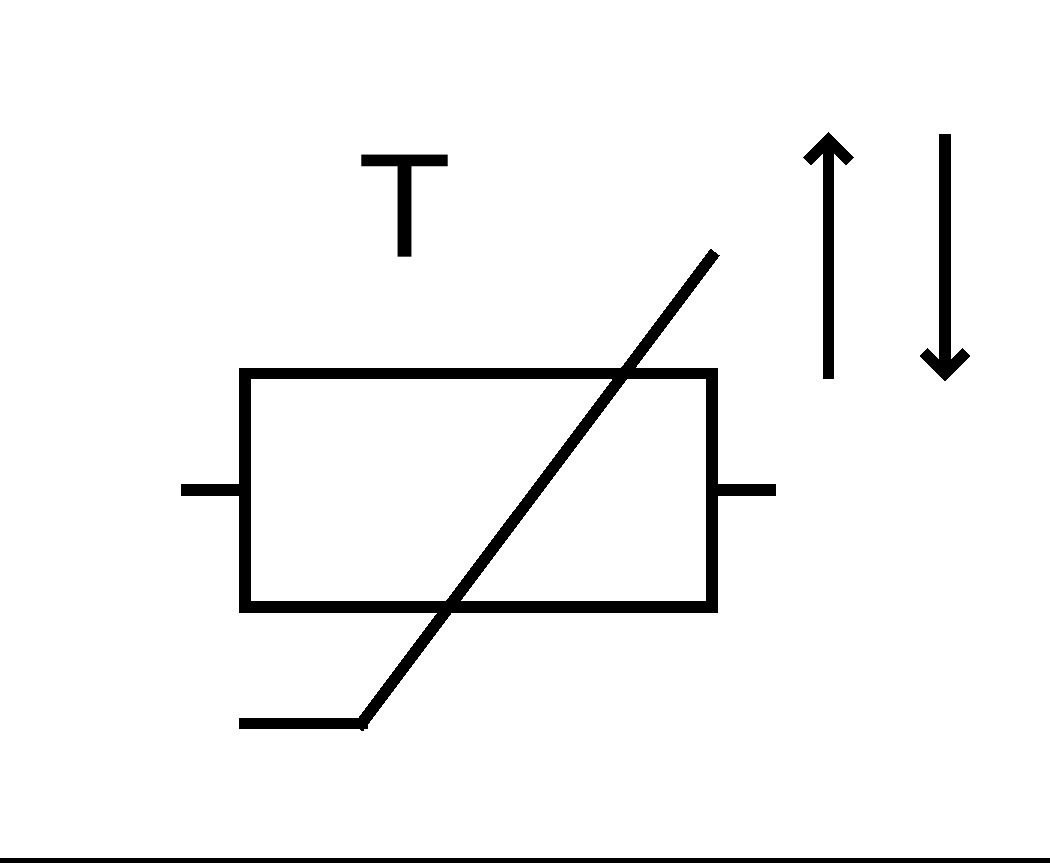
\includegraphics[width=\textwidth]{./pics/ntc-schaltsymbol.png}
		\end{minipage}
	\end{minipage}
	
	\bigskip
	\emph{Anmerkung:}
	
	Es gibt auch Kaltleiter, kurz: \textbf{PTC} (\emph{engl. \textbf{p}ositive \textbf{t}emperature \textbf{c}oefficient}), die ihren Widerstand verringern, wenn es kälter wird, und erhöhen, wenn es wärmer wird. Zusammen genommen bezeichnet man NTC's und PTC's auch als Thermistoren, also als temperaturabhängige Widerstände (engl. \textbf{therm}ally sensitive res\textbf{istor}).
\end{zsfg}

\newpage
\section{Schaltungen mit Transistoren steuern}
\label{sec:transistor}

Manche Projekte wie die \hyperref[proj:strassenlampe]{Straßenlampe} benötigt nur ein sehr simples Programm in der Form WENN - DANN - SONST. Für solche Fälle ist der Arduino eigentlich eine überdimensionierte Lösung - viel einfacher, jedenfalls in Bezug auf die Anzahl der Bauteile, ist die Umsetzung dieser Schaltung mithilfe eines Transistors. Dieser ist (unter anderem) ein elektronischer Schalter, mit dem sich das WENN - DANN - SONST - Verhalten ganz ohne Programm umsetzen lässt.

\begin{ziel}
	\textbf{Frage:} Wie verwendet man einen Transistor?
\end{ziel}

\medskip
\begin{minipage}{0.85\textwidth}
	Ein Transistor hat drei Anschlüsse, die als Kollektor (\textbf{C} von engl. \emph{collector}), Basis (\textbf{B}) und Emitter (\textbf{E}) bezeichnet werden. Wenn man auf die abgeflachte Seite des Transistors schaut, sind die drei Pins in der genannten Reihenfolge angeordnet. Im Folgenden geht es zunächst um deren Grundfunktionen.
\end{minipage}
\hfill
\begin{minipage}{0.13\textwidth}
	\centering
	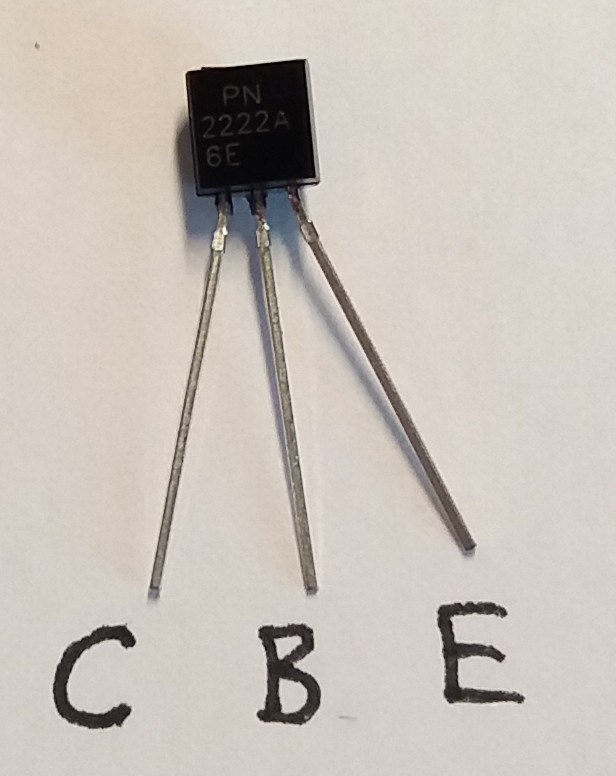
\includegraphics[width=0.77\textwidth]{./pics/transistor.jpg}
\end{minipage}

\medskip

\begin{aufgabe} \emph{Digitalpins verstehen}
	
	Befolge die unten angegebenen Schritte und stelle Schlussfolgerungen über die Funktionsweise eines Transistors an. Erkennst du Gemeinsamkeiten zu digitalen Pins?
	\begin{enumerate}[label=\alph*), itemsep=0mm,parsep=0mm]
		\item Baue die unten abgebildeten Schaltungen nacheinander auf. Spiele für die zweite Schaltung ein einfaches Blink-Programm auf den Arduino.
		\begin{figure}[H]
			\centering
			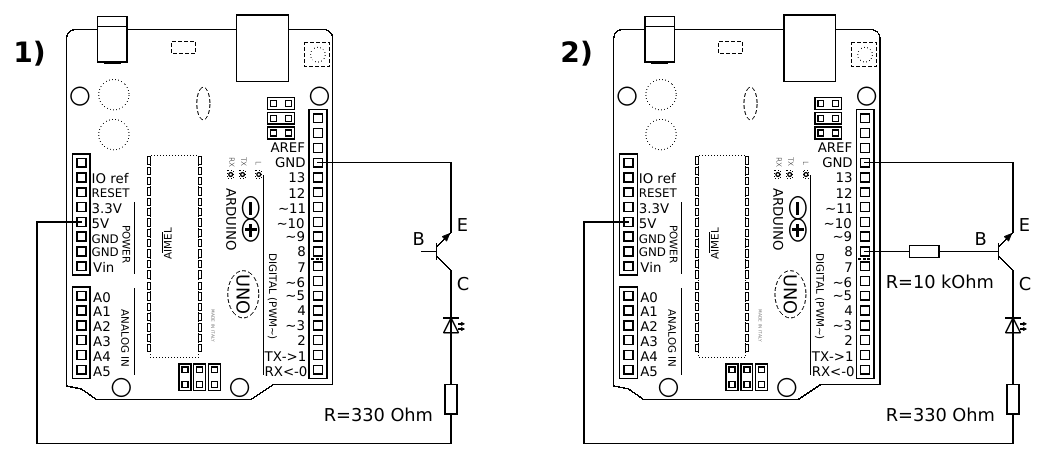
\includegraphics[width=0.75\textwidth]{./Zeichnungen/Schaltplan-Transistor-verstehen.png}
		\end{figure}
		\item Ersetze den $\SI{10}{\kilo\ohm}$ Widerstand durch einen $\SI{100}{\kilo\ohm}$ Widerstand.
	\end{enumerate}
\end{aufgabe}

\begin{aufgabe} \emph{Vermessung}
	
	\medskip
	\begin{minipage}{0.58\textwidth}
		Um den Transistor zielgerichtet nutzen zu können, muss man die Spannung $U_{BE}$ zwischen Basis und Emitter kennen, bei der der Transistor anfängt, durchzuschalten. Dazu dient die rechts abgebildete Schaltung.
		
		Das Potentiometer lässt sich wieder in zwei Teilwiderstände $R_1$ und $R_2$ zerlegen, an denen die Spannung $U_1$ bzw. $U_2$ abfällt. Erkläre, wie der Widerstand $R_2$ und die Spannung $U_{BE}$ zusammenhängen.
	\end{minipage}
	\hfill
	\begin{minipage}{0.38\textwidth}
		\centering
		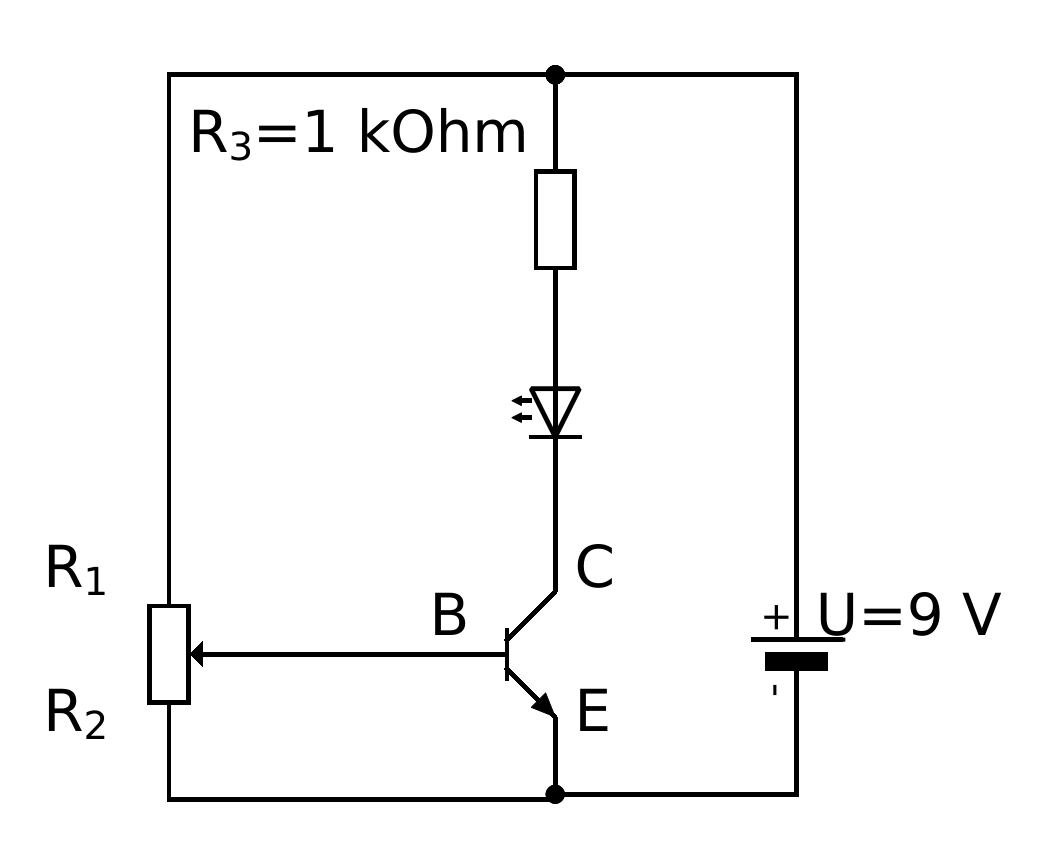
\includegraphics[width=\textwidth]{./Zeichnungen/Schaltplan-U-BE-Messung1.png}
	\end{minipage}
	
	\begin{minipage}[c][8cm][t]{0.58\textwidth}
		Baue die Schaltung nun auf. Um die Spannung $U_{BE}$ messen zu können, wird ein Arduino ergänzt, der die Spannung in A0 ausliest und auf dem seriellen Monitor ausgibt. 
		
		Bestimme so die Grenzspannung $U_{BE}$, ab der der Transistor anfängt zu schalten, sodass die LED leuchtet.
		
		\begin{center}
			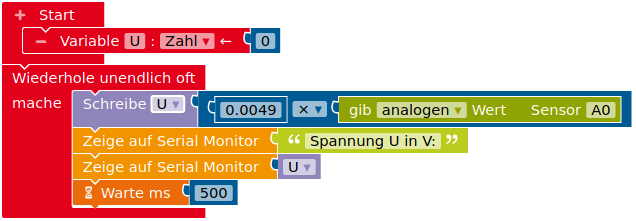
\includegraphics[width=\textwidth]{./pics/spannung-an-transistor-messen.png}
		\end{center}
	\end{minipage}
	\hfill
	\begin{minipage}[c][8cm][t]{0.38\textwidth}
		\centering
		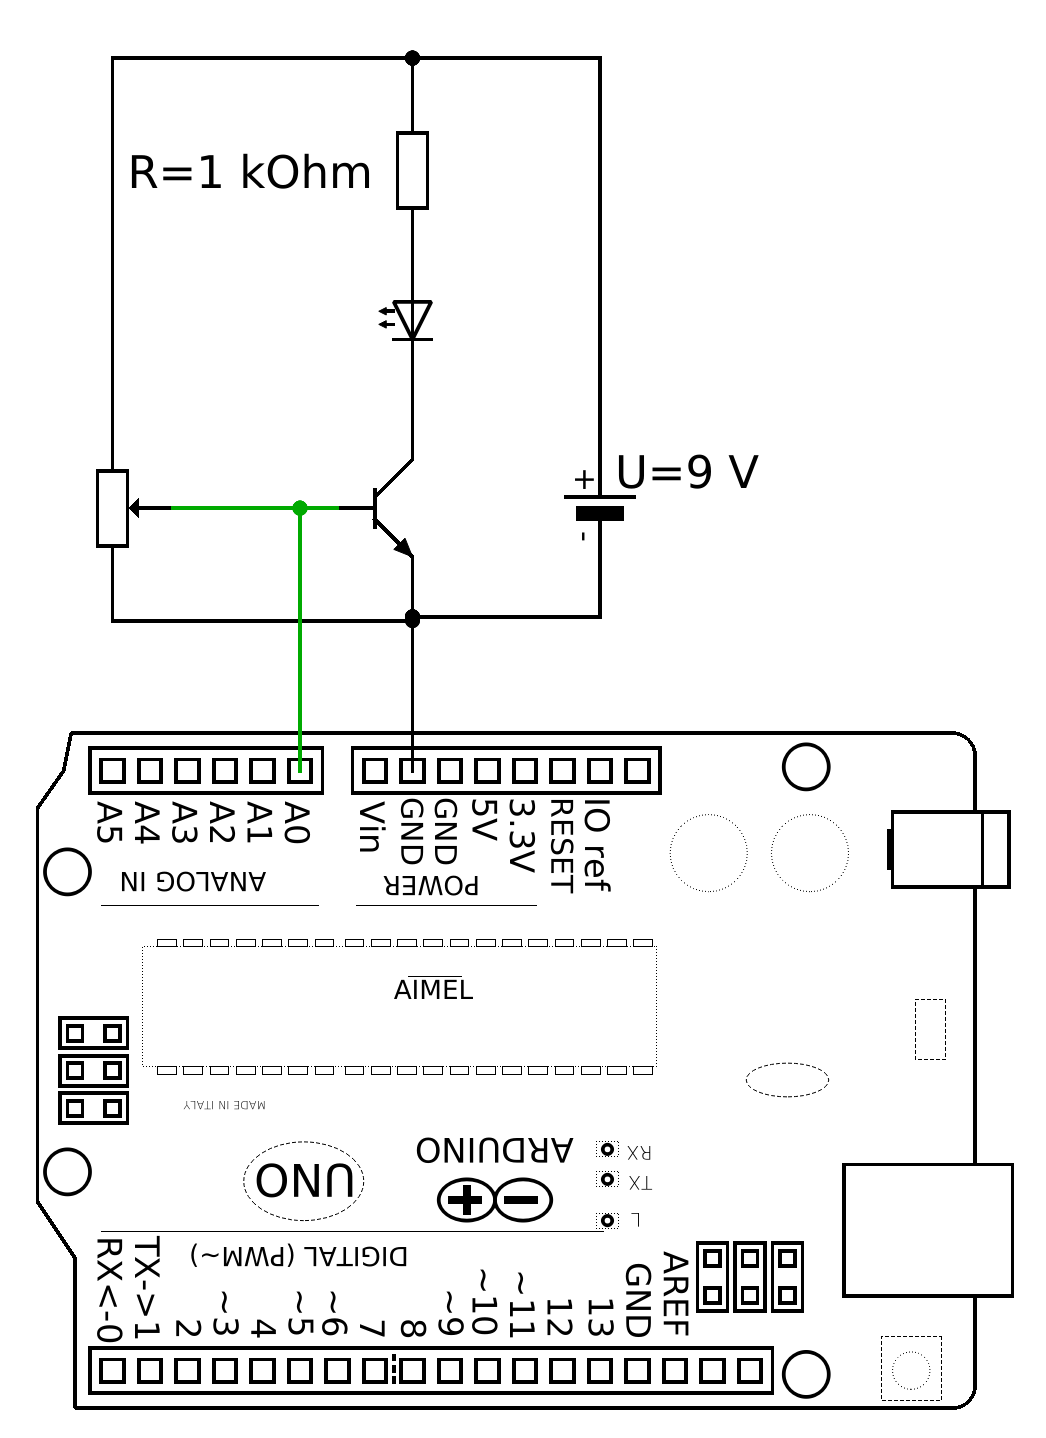
\includegraphics[width=\textwidth]{./Zeichnungen/Schaltplan-U-BE-Messung.png}
	\end{minipage}
\end{aufgabe}

\begin{projekt}[Straßenlampe ohne Mikrocontroller\label{proj:strassenlampeomc}]
	\begin{minipage}{0.58\textwidth}
		Nun kann die Straßenlampe auch ohne Arduino realisiert werden. Dazu wird statt des Potentiometers ein Spannungsteiler mit einem LDR und einem Festwiderstand aufgebaut (siehe Schaltplan rechts).
		
		Bestimme die Größe des Festwiderstands $R_F$ so, dass der Transistor schaltet, wenn die Größe des LDR $R_{LDR}=\SI{7}{\kilo\ohm}$ beträgt.
		
		\emph{Tipps:}
		\begin{itemize}[itemsep=0mm, parsep=0mm]
			\item Nutze die Spannungsteilerformel.
			\item Nutze $U_{LDR}=U_{BE}$. Ab welcher Spannung schaltet der Transistor?
		\end{itemize}
	\end{minipage}
	\hfill
	\begin{minipage}{0.4\textwidth}
		\centering
		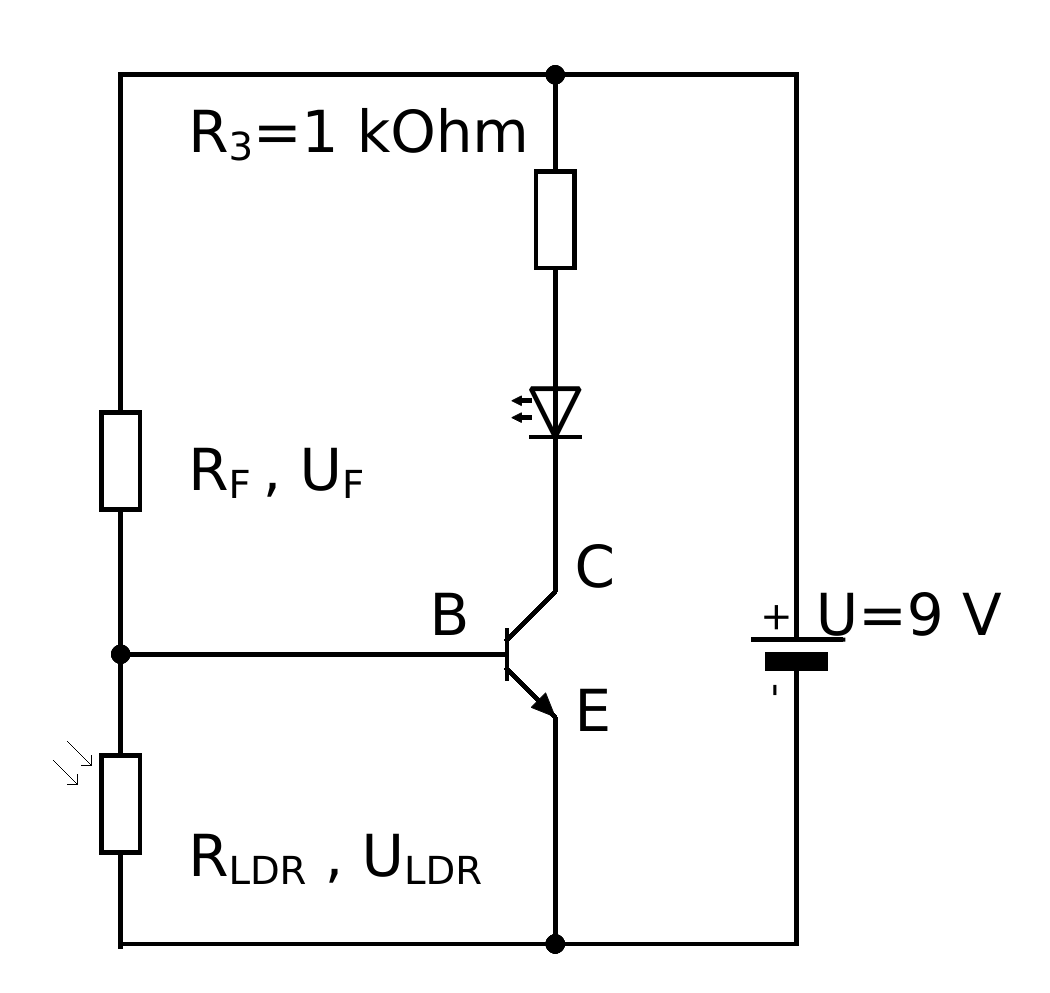
\includegraphics[width=\textwidth]{./Zeichnungen/Schaltplan-Strassenlampe-ohne-mC.png}
	\end{minipage}
	
	\bigskip
	Baue die Schaltung danach auf und teste sie.
\end{projekt}

\begin{zsfg}{Der Transistor}
	
	\medskip
	\begin{minipage}{0.7\textwidth}
		Ein Transistor hat drei Anschlüsse, die als Kollektor (\textbf{C} von engl. \emph{collector}), Basis (\textbf{B}) und Emitter (\textbf{E}) bezeichnet werden. Wenn man auf die abgeflachte Seite des Transistors schaut, sind die drei Pins in der genannten Reihenfolge angeordnet.
	\end{minipage}
	\hfill
	\begin{minipage}{0.28\textwidth}
		\begin{minipage}{0.48\textwidth}
			\centering
			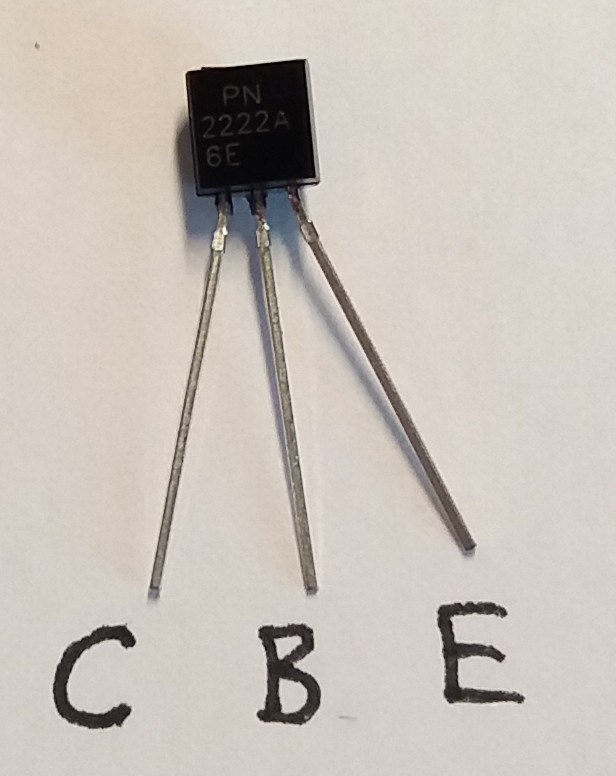
\includegraphics[width=0.9\textwidth, height=2cm]{./pics/transistor.jpg}
		\end{minipage}
		\hfill
		\begin{minipage}{0.48\textwidth}
			\centering
			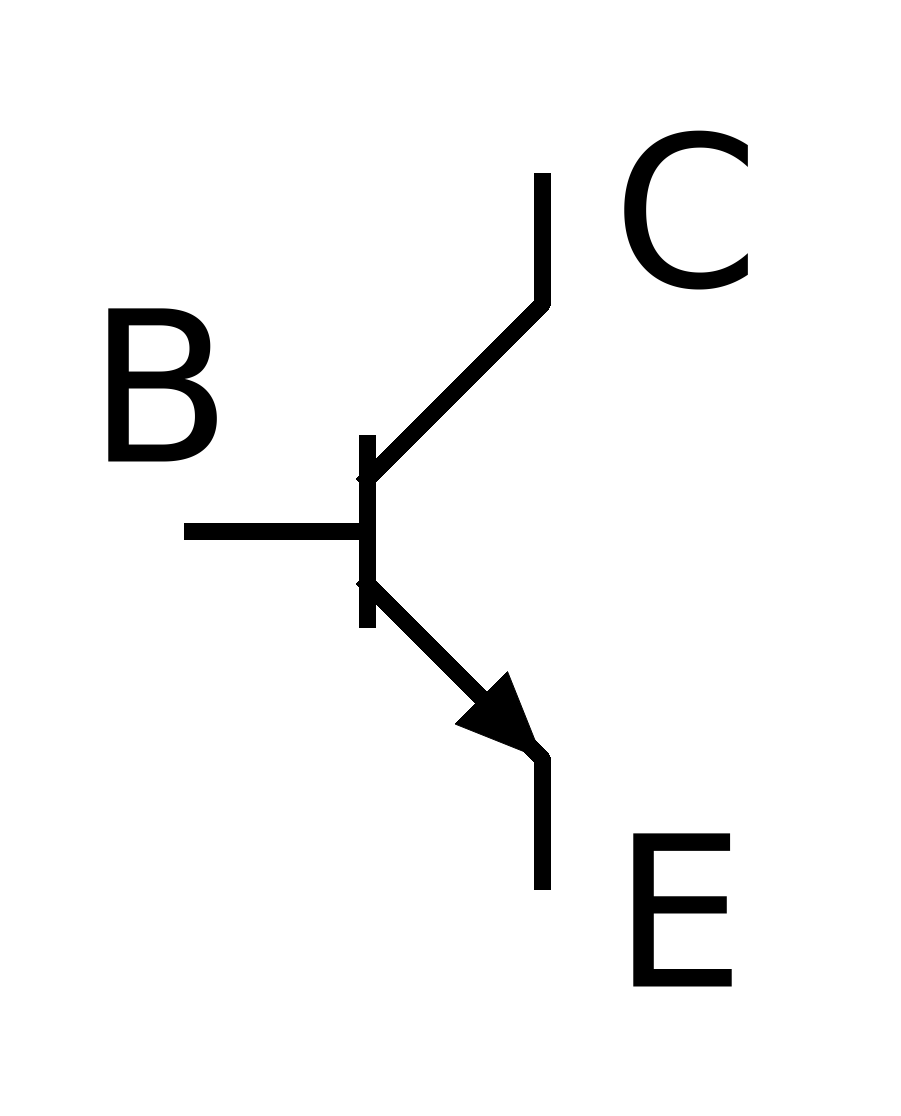
\includegraphics[width=0.9\textwidth, height=2cm]{./pics/transistor-schaltsymbol.png}
		\end{minipage}
	\end{minipage}
	
	\medskip
	Transistoren dienen als elektronische Schalter oder Verstärker (letzteres wird im Abschnitt \ref{sec:motoren} zu Motoren genutzt). Als Schalter lassen sie sich nutzen, weil die Strecke vom Kollektor zum Emitter ohne Weiteres nicht leitet. Erst wenn zwischen Basis und Emitter eine Spannung $U_{BE} \approx \SI{0,6}{\volt}$ anliegt, fließt \emph{zwischen Basis und Emitter ein schwacher Strom}, der den Transistor mit Elektronen flutet und es dadurch ermöglicht, dass \emph{zwischen Kollektor und Emitter ein starker Strom} fließen kann.
	
	Die Möglichkeit, mit Transistoren automatisierte Schalter herzustellen und dadurch Programme physikalisch abzubilden, macht Transistoren zur Grundlage von Mikrocontrollern und Computern und damit zu einer der wichtigsten Erfindungen des 20. Jahrhunderts. Schon auf dem kleinen integrierten Schaltkreis des Arduino, dem ATMEGA328P, sind Millionen von Transistoren verbaut. Wenn ein Digitalpin des Arduino auf HIGH gestellt wird, dann wird intern ein Transistor geschaltet.
	
	Es gibt verschiedene Bauarten für Transistoren. Im hier verwendeten Starter Kit sind zwei npn-Transistoren (Pn2222) vorhanden, was bedeutet, dass darin zwei n-dotierte und eine p-dotierte Schicht in der Mitte verbaut sind. npn-Transistoren müssen mit einer n-Schicht (normalerweise der Emitter) mit GND verbunden sein.
\end{zsfg}

\newpage
\section{Elektromotor und Diode}\label{sec:motoren}

Bei vielen Projekten soll sich etwas bewegen - dies lässt sich mit Elektromotoren realisieren. Die Ansteuerung eines Elektromotors erfordert auf der Hardware-Seite ein wenig Vorbereitung, denn aufgrund der hohen Ströme, die Elektromotoren ziehen, sollte man sie nicht direkt an den Digitalpins des Arduino anschließen. Für die Steuerung greift man meistens auf einen Transistor zurück; eine brauchbare Alternative ist aber auch das Relais. Beide Steuerungsmöglichkeiten werden im Folgenden erarbeitet.

\begin{ziel}
	\textbf{Frage:} Wie betreibt man einen Elektromotor am Arduino?
\end{ziel}
\medskip
\begin{minipage}[t]{0.5\textwidth}
	\begin{aufgabe} \emph{Motor und Diode - ein Paar, das zusammen gehört}
		
		Erkläre die Funktion der Diode parallel zum E-Motor in eigenen Worten. Lies dazu die Hintergrundinformationen zum Elektromotor und zur Diode.
		
		\smallskip
		Baue die rechts abgebildete Schaltung zum Betrieb eines Gleichstrom-Elektromotors am Arduino auf.
		
		\bigskip
		\ausrufezeichen \emph{Es ist sehr wichtig, dass die Diode richtig, also in Sperrrichtung, eingebaut wird, da sonst der Arduino zerstört werden könnte!}
	\end{aufgabe}
\end{minipage}
\hfill
\begin{minipage}[t]{0.45\textwidth}
	\begin{figure}[H]
		\centering
		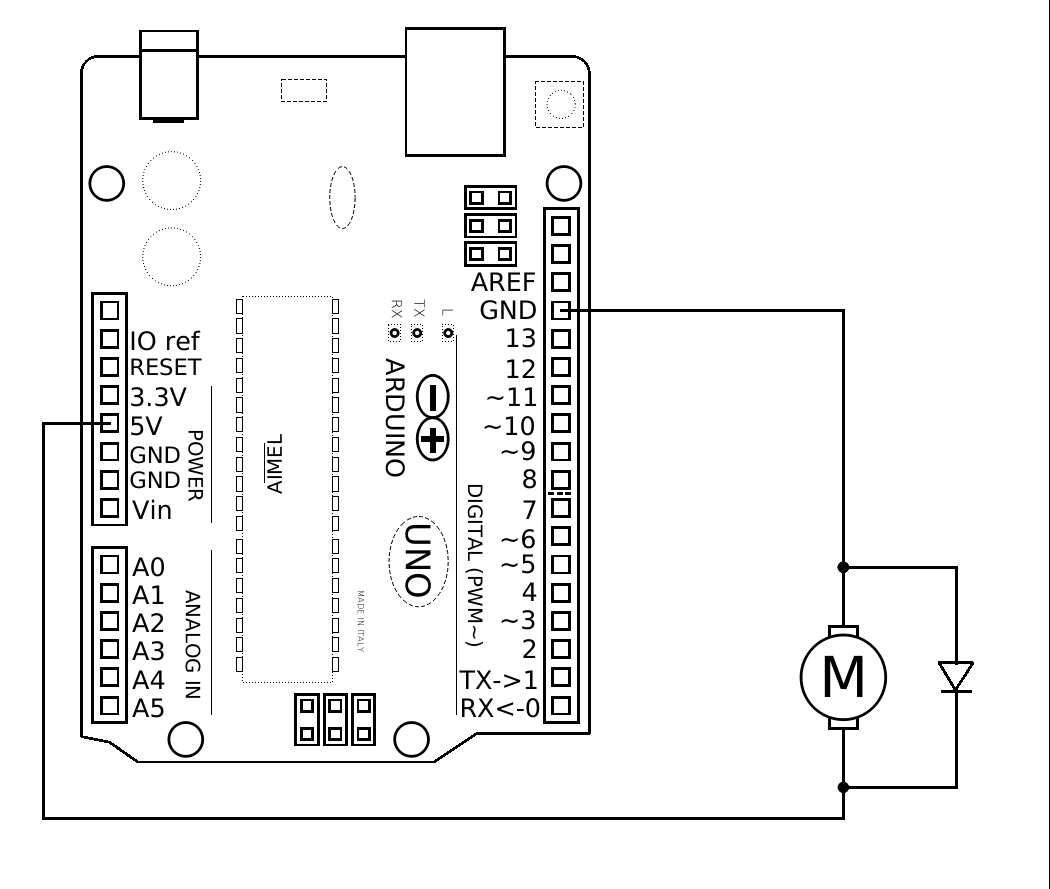
\includegraphics[width=0.95\textwidth]{./Zeichnungen/Schaltplan-Motoranschluss-einfach.png}
		\caption{Anschluss eines Gleichstrom-Elektromotors mit dem Arduino als Spannungsquelle.}
	\end{figure}
\end{minipage}
\medskip

\emph{Hintergrundinformationen:}
\medskip

\begin{zsfg}{Elektromotor}
	\begin{wrapfigure}{r}{0.38\textwidth}
		\vspace{-0.7\baselineskip}
		\centering
		\hfill
		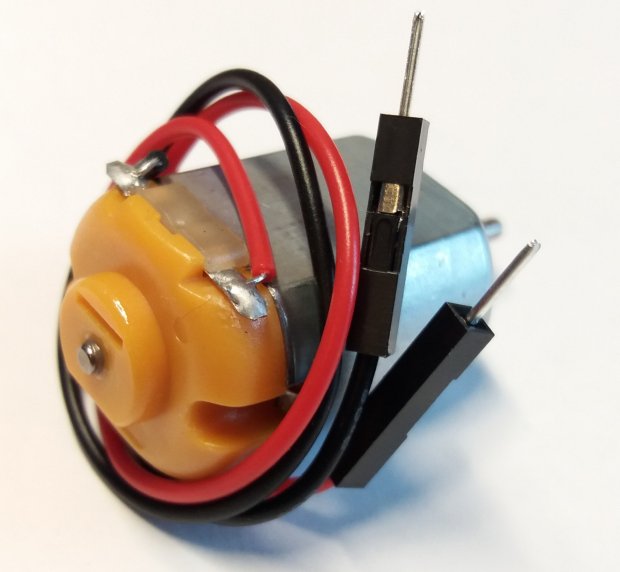
\includegraphics[width=0.21\textwidth]{./pics/dc-motor-klein.png}
		\hfill
		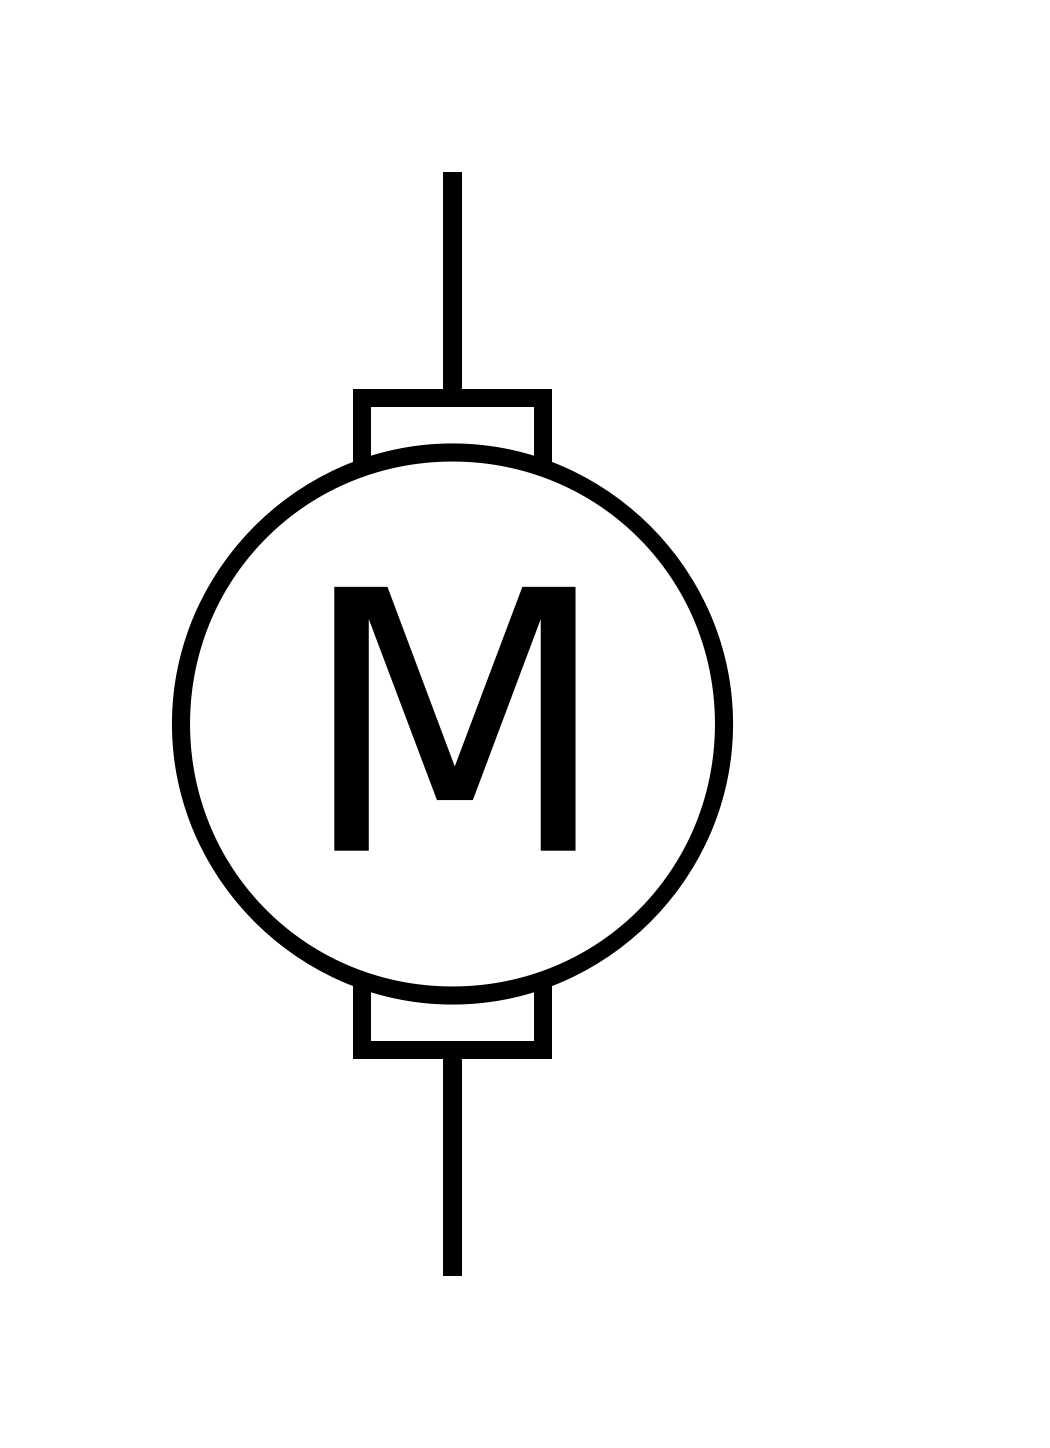
\includegraphics[width=0.13\textwidth]{./Zeichnungen/motor-schaltsym.png}
		\hfill
		\caption{Gleichstrom-Elektromotor in real und als Schaltsymbol.}
	\end{wrapfigure}
	Ein \textbf{Elektromotor} besteht aus mehreren Spulen und Magneten. Wenn Strom durch die Spulen fließt, baut sich um die Spulen ein Magnetfeld auf, das mit dem Magnetfeld der eingebauten Magneten wechselwirkt (Anziehung/Abstoßung), sodass es zu einer Drehung des Motors kommt. Ein sogenannter Kommutator sorgt dafür, dass der Strom durch die Spulen ständig seine Richtung wechselt, sodass es immer wieder von Neuem zu Anziehung bzw. Abstoßung der Magnetfelder kommt und die Drehung nicht aufhört, solange eine Spannung anliegt.
\end{zsfg}

%\medskip
%\begin{minipage}{0.6\textwidth}
%	Ein Elektromotor besteht aus mehreren Spulen und Magneten. Wenn Strom durch die Spulen fließt, baut sich um die Spulen ein Magnetfeld auf, das mit dem Magnetfeld der eingebauten Magneten wechselwirkt (Anziehung/Abstoßung), sodass es zu einer Drehung des Motors kommt. Ein sogenannter Kommutator sorgt dafür, dass der Strom durch die Spulen ständig seine Richtung wechselt, sodass es immer wieder von Neuem zu Anziehung bzw. Abstoßung der Magnetfelder kommt und die Drehung nicht aufhört, solange eine Spannung anliegt.
%\end{minipage}
%\hfill
%\begin{minipage}{0.38\textwidth}
%	\centering
%	\hfill
%	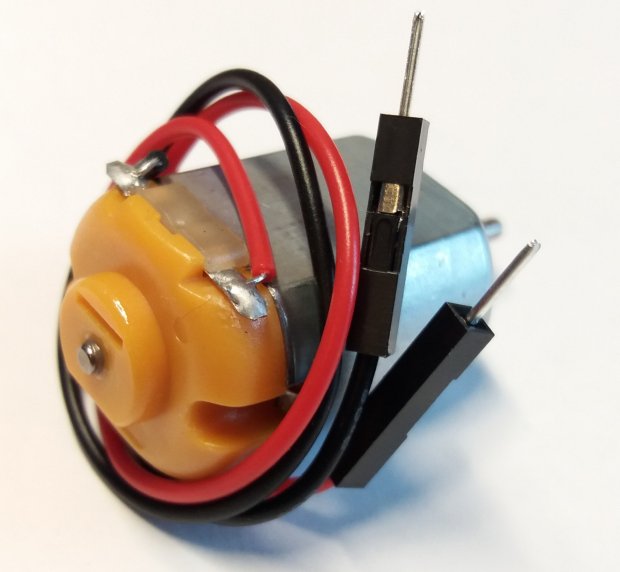
\includegraphics[width=0.55\textwidth]{./pics/dc-motor-klein.png}
%	\hfill
%	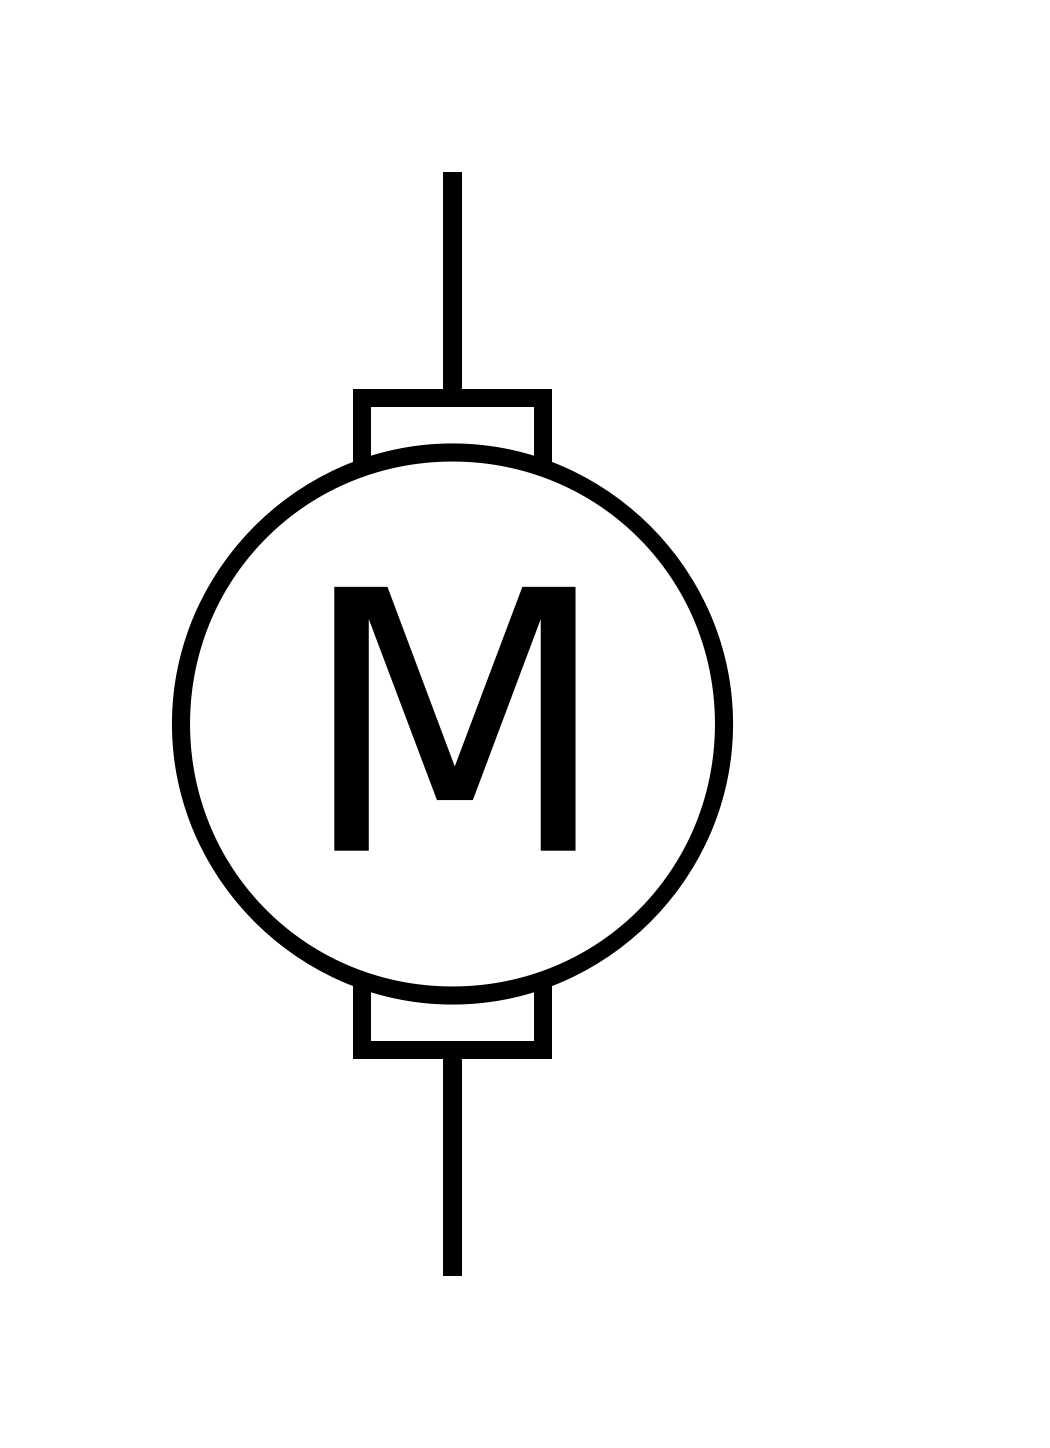
\includegraphics[width=0.35\linewidth]{./Zeichnungen/motor-schaltsym.png}
%	\hfill
%\end{minipage}
%\medskip

Wenn keine Spannung mehr am Motor anliegt, wird sich der Motor aufgrund seiner Trägheit immer noch ein wenig weiterdrehen. Durch das Drehen der Spulen im Magnetfeld der eingebauten Permanentmagneten wird in den Spulen ein Strom induziert, dessen Richtung entgegengesetzt zur vorherigen Richtung ist. Dieser \enquote{falsch} gerichtete Strom würde den Arduino zerstören. Aus diesem Grund schaltet man eine \emph{Diode} parallel zum Motor.

\begin{zsfg}{Diode}
	\begin{wrapfigure}{r}{0.28\textwidth}
		\vspace{-0.5\baselineskip}
		\centering
		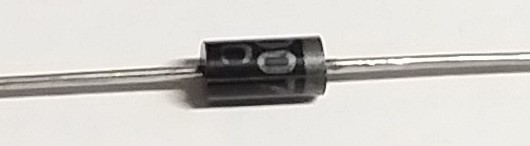
\includegraphics[width=0.75\linewidth]{./pics/diode2.jpg}
		
		\vspace{-0.5\baselineskip}
		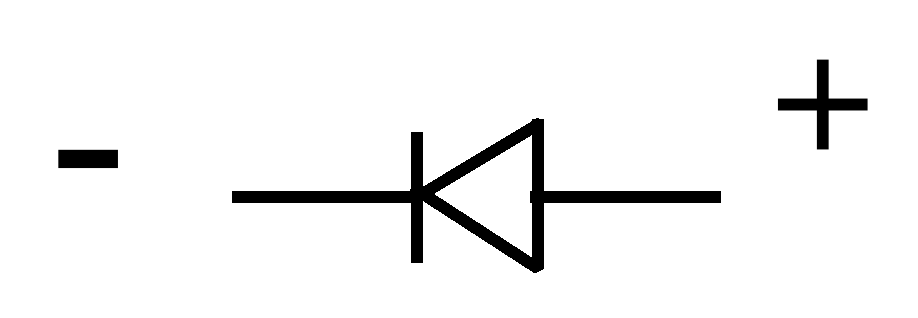
\includegraphics[width=0.75\linewidth,angle=180]{./Zeichnungen/diode-schaltsym.png}
		\caption{Diode in real und als Schaltsymbol.}
	\end{wrapfigure}
	Eine \textbf{Diode} ist wie ein elektrisches Ventil: Sie lässt den Strom nur in eine Richtung durch. Im Gegensatz zu Leuchtdioden wandeln \enquote{normale} Dioden die elektrische Energie in Wärme um. In \emph{Durchlassrichtung} wird der negative Pol (bzw. GND) mit der Seite verbunden, an der der Ring angebracht ist, und der positive Pol mit der anderen Seite.
	\bigskip
\end{zsfg}

%\medskip
%\begin{minipage}{0.7\textwidth}
%	 Eine Diode ist wie ein elektrisches Ventil: Sie lässt den Strom nur in einer Richtung durch. Im Gegensatz zu Leuchtdioden wandeln \enquote{normale} Dioden die elektrische Energie in Wärme um. In Durchlassrichtung wird der negative Pol (bzw. GND) mit der Seite verbunden, an der der Ring angebracht ist, und der positive Pol mit der anderen Seite.
%\end{minipage}
%\hfill
%\begin{minipage}{0.28\textwidth}
%	\begin{figure}[H]
%		\centering
%		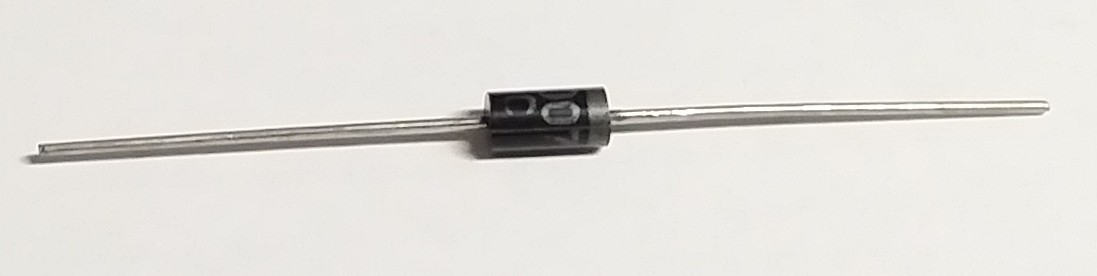
\includegraphics[width=0.75\linewidth]{./pics/diode.jpg}
%		
%%		\vspace{-1.5\baselineskip}
%		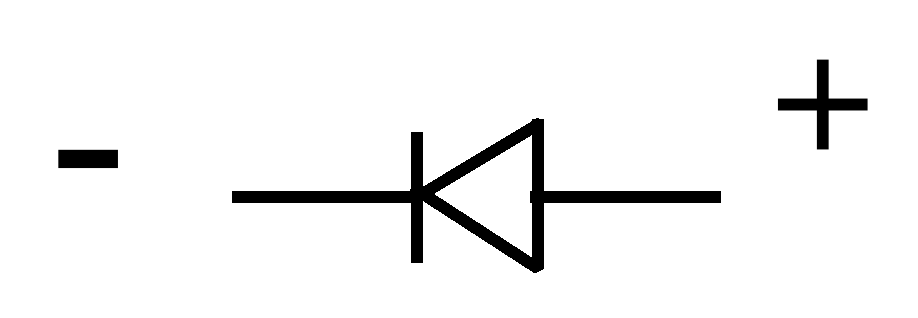
\includegraphics[width=0.75\linewidth,angle=180]{./Zeichnungen/diode-schaltsym.png}
%		\caption{Diode in real und als Schaltsymbol.}
%	\end{figure}
%\end{minipage}
%\medskip

Die Diode wird jedoch \emph{Sperrrichtung} eingebaut, also so, dass der Ring mit 5V und die andere Seite mit GND verbunden ist. Dadurch fließt im Normalbetrieb kein Strom durch die Diode. Wenn jedoch der entgegengerichtete Induktionsstrom des Motors auftritt, kann dieser durch die Diode abfließen, bis die verbleibende elektrische Energie vollständig in Wärme umgewandelt wurde.

\begin{recherche}{Verpolungsschutz}
	LEDs leuchten nicht, wenn man sie falsch herum anschließt. Andere Bauteile wie Elektrolytkondensatoren explodieren sogar, wenn man sie falsch herum anschließt. Um zu vermeiden, dass solche Schäden entstehen, wenn man eine Batterie falsch herum anschließt, werden in einigen Fällen Dioden genutzt. Recherchiere im \href{https://www.elektronik-kompendium.de/sites/slt/1206251.htm}{Elektronik-Kompendium},\footnote{\url{https://www.elektronik-kompendium.de/sites/slt/1206251.htm}} wie dies funktioniert.
\end{recherche}

\begin{recherche}{Aufbau von Gleichstrom-Elektromotoren}
	Oben wurde die Funktionsweise von Gleichstrom-Elektromotoren bereits angedeutet. Recherchiere im Internet den genauen Aufbau und Ablauf der Drehbewegung. 
\end{recherche}

\newpage
\subsection{Elektromotor mit Transistor steuern}
% Steuerung mit Transistor

Der 5\,V-Pin des Arduino liefert zwar in vielen Fällen genügend Strom für den Motor, jedoch lässt er sich nicht programmieren. Dazu lässt sich ein Transistor einbauen.

\begin{ziel}
	\textbf{Frage:} Wie steuert man einen Elektromotor mit einem Transistor am Arduino?
\end{ziel}


\medskip
\begin{minipage}{0.48\textwidth}
	Die rechts abgebildete Schaltung zeigt, wie ein npn-Transistor eingebaut werden kann, um den Motor mithilfe von Digitalpin 9 zu schalten. Der Transistor lässt den Strom zwischen Emitter (E) und Kollektor (C) passieren, wenn die Spannung zwischen Basis (B) und Emitter (E) mehr als 0,7\,V beträgt, anderenfalls sperrt er. Der Vorwiderstand mit $R=\SI{330}{\ohm}$ sorgt dafür, dass der Basisstrom nicht zu groß wird.
	
	Es ist ratsam, die Basis mit einem PWM-Pin (gekennzeichnet durch $\sim$) zu verbinden, da sich dadurch die Geschwindigkeit des Motors steuern lässt.
\end{minipage}
\hfill
\begin{minipage}{0.48\textwidth}
	\begin{figure}[H]
		\centering
		\includegraphics[width=\textwidth]{./Zeichnungen/motoranschluss-mit-steuerung.png}
		\caption{Anschluss eines Gleichstrom-Elektromotors am Arduino mit Steuerung über einen Transistor an Digitalpin 9.}
	\end{figure}
\end{minipage}
\marginpar{%
	\scriptsize
	\centering
	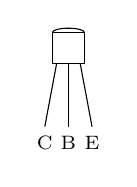
\begin{tikzpicture}
	\draw (-0.2,0.8) rectangle (0.2,1.2);
	\draw (0.2,1.2) arc [start angle=0,end angle=180,x radius=0.2,y radius=0.05];
	\draw (-0.15,0.8) -- (-0.3,0) node [below] {\scriptsize C};
	\draw (0,0.8) -- (0,0) node [below] {\scriptsize B};
	\draw (0.15,0.8) -- (0.3,0) node [below] {\scriptsize E};
	\end{tikzpicture}
	
	npn-Transistor; Blick auf flache Seite
}

\begin{aufgabe}
	
	Baue die oben abgebildete Schaltung auf und probiere die Steuerung des Motors mittels Pulsweitenmodulation aus.
	
	\begin{figure}[H]
		\centering
		\includegraphics[width=0.5\linewidth]{./pics/pwm-motorsteuerung.png}
	\end{figure}
	
	Simuliere mit dem Motor eine konstant beschleunigende Bewegung (\emph{vgl. \href{sec:pwm}{Fading}}), gefolgt von einer abrupten Bremsung.
\end{aufgabe}

\begin{projekt}[Automatischer Lüfter]\label{proj:luefter}
	Baue einen Lüfter, der anspringt, wenn die Temperatur größer als $\SI{30}{\celsius}$ wird. Probiere deine Schaltung durch Anfassen des NTC aus.
	
	\emph{Erweiterung:} Programmiere die Schaltung so, dass der Lüfter sich umso schneller dreht, je höher die Temperatur ist.
\end{projekt}

\newpage
%\medskip
\emph{Schaltung mit externer Spannungsquelle}
\medskip

\begin{minipage}{0.5\textwidth}
	Wenn der verwendete Elektromotor größer ist und mehr Strom zieht bzw. größere Spannungen benötigt, muss für den Elektromotor eine eigene Spannungsquelle verwendet werden, die genügend Spannung und Strom bieten kann. Der rechts abgebildete Schaltplan zeigt, wie der Aufbau dann vorzunehmen ist. Wichtig ist dabei, dass ein gemeinsames GND-Niveau hergestellt wird - vergleichbar einem \enquote{Normalnull} für die Höhenangaben, hier allerdings als \enquote{Normalnull} für das elektrische Potenzial.
	
	Der Arduino kann über USB oder eine zweite Batterie mit Strom versorgt werden.
\end{minipage}
\hfill
\begin{minipage}{0.48\textwidth}
	\begin{figure}[H]
		\centering
		\includegraphics[width=\textwidth]{./Zeichnungen/Schaltplan-Motoranschluss-ext-Spannung.png}
		\caption{Anschluss eines Gleichstrom-Elektromotors am Arduino mit Steuerung über einen Transistor und mit externer Spannungsquelle für den Motor.}
	\end{figure}
\end{minipage}

%\newpage
\vspace{2\baselineskip}
\subsection{Elektromotor mit Relais steuern}
% Steuerung von Motor mit Relais, Vgl zu Transistor-Schaltung

Wie oben zu sehen, muss der Arbeitsstromkreis mit dem Motor und der Steuerstromkreis mit dem Arduino bei Verwendung eines Transistors immer miteinander verbunden bleiben - auch bei sehr großen Stromstärken. Damit verbleibt immer eine gewisse Gefahr, dass eine Spannungsspitze auf den Arduino durchschlägt und ihn zerstört. Mit einem Relais lässt sich dieses Risiko vermeiden. Ein weiterer Vorteil ist, dass der Arbeitsstromkreis auch mit Wechselstrom betrieben werden kann, wenn ein Relais als Schalter genutzt wird.

\begin{ziel}
	\textbf{Frage:} Wie verwendet man ein Relais am Arduino?
\end{ziel}

Ein Relais (siehe unten, grau unterlegt) besteht im Wesentlichen aus einer Spule mit Eisenkern und einem Wechselschalter, an dem eine Feder angebracht ist.

\bigskip
% Aufbau Relais (mit Zeichnung für beide Zustände des Wechselschalters)
\begin{minipage}{0.48\textwidth}
	\begin{figure}[H]
		\centering
		%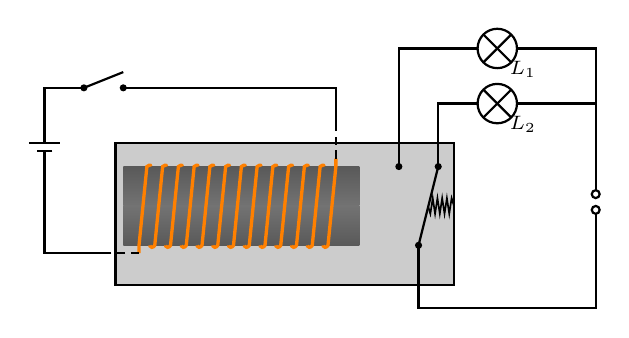
\begin{tikzpicture}
	% Kasten für Relais
	\draw [thick,fill=gray!40] (-0.1,-0.5) rectangle (4.2,1.3);
	%Eisenkern
	\shade [top color=gray!70!black, bottom color=gray!90!black] (0,0.5) rectangle (3,1);
	\shade [bottom color=gray!70!black, top color=gray!90!black] (0,0) rectangle (3,0.5);
	% Spule
	%Anfangspunkt (0.2,-0.1)
	\draw [color=orange, very thick] (0.2,-0.1) -- (0.2,0) -- ++(0.1,1) .. controls ++(0.05,0.04) and ++(0,0) .. ++(0.05,0);
	\foreach \x in {0.4,0.6,...,2.6} {
		\draw [color=orange, very thick] (\x-0.06,0) -- (\x-0.06,-0.01) .. controls ++(0.03,-0.04) and ++(0,0) .. (\x,0) -- ++(0.1,1) .. controls ++(0.05,0.04) and ++(0,0) .. ++(0.05,0);
	}
	\draw [color=orange, very thick] (2.6-0.06,0) -- (2.6-0.06,-0.01) .. controls ++(0.03,-0.04) and ++(0,0) .. (2.6,0) -- ++(0.1,1) -- ++(0,0.1);  % Endpunkt: (2.7,1.1)
	%%%% Steuerstromkreis
	\draw (2.7,1.1) [densely dashed, thick] -- (2.7,1.5);
	\draw [thick] (2.7,1.5) -- (2.7,2) -- (0,2);
	%Schalter offen
	\draw [thick,fill=black] (0,2) circle [radius=0.03]; 
	\draw [thick] (-0.5,2) -- ++ (0.5,0.2);
	\draw [thick,fill=black] (-0.5,2) circle [radius=0.03]; 
	\draw [thick] (-0.5,2) -- (-1,2) -- (-1,1.3) ++(-0.2,0) -- ++(0.4,0) ++(-0.1,-0.1) -- ++(-0.2,0) ++(0.1,0) -- (-1,-0.1) -- (-0.2,-0.1);
	\draw [thick,densely dashed] (0.2,-0.1) -- (-0.2,-0.1);
	%%%% Arbeitsstromkreis
	%Wechselschalter
	\draw [thick, fill=black] (3.75,0) circle [radius=0.03];
	\draw [thick, fill=black] (3.5,1) circle [radius=0.03];
	\draw [thick, fill=black] (4,1) circle [radius=0.03];
	\draw [thick] (3.75,0) -- (4,1);
	%Feder
	\draw [semithick] (4.2,0.5) -- ++(-0.03,0.1) -- ++(-0.03,-0.2) -- ++(-0.03,0.2) -- ++(-0.03,-0.2) -- ++(-0.03,0.2) -- ++(-0.03,-0.2)-- ++(-0.03,0.2) -- ++(-0.03,-0.2)-- ++(-0.03,0.2) -- ++(-0.03,-0.2) -- ++(-0.03,0.1);
	% Stromkreis an sich
	\draw [thick] (3.75,0) -- (3.75,-0.8) -- (6,-0.8) -- (6,0.4);
	\draw [thick] (6,0.45) circle [radius=0.05];
	\draw [thick] (4,1) -- (4,1.8) -- (4.5,1.8);
	\draw [thick] (4.75,1.8) circle [radius=0.25] node [below right =0.8] {\scriptsize $L_2$};
	\draw [thick] (4.75,1.8) -- ++(45:0.25);
	\draw [thick] (4.75,1.8) -- ++(135:0.25);
	\draw [thick] (4.75,1.8) -- ++(225:0.25);
	\draw [thick] (4.75,1.8) -- ++(315:0.25);
	\draw [thick] (5,1.8) -- (6,1.8) -- (6,0.7);
	\draw [thick] (6,0.65) circle [radius=0.05];
	\draw [thick] (3.5,1) -- (3.5,2.5) -- (4.5,2.5);
	\draw [thick] (4.75,2.5) circle [radius=0.25] node [below right =0.8] {\scriptsize $L_1$};
	\draw [thick] (4.75,2.5) -- ++(45:0.25);
	\draw [thick] (4.75,2.5) -- ++(135:0.25);
	\draw [thick] (4.75,2.5) -- ++(225:0.25);
	\draw [thick] (4.75,2.5) -- ++(315:0.25);
	\draw [thick] (5,2.5) -- (6,2.5) -- (6,1.8);
\end{tikzpicture}
		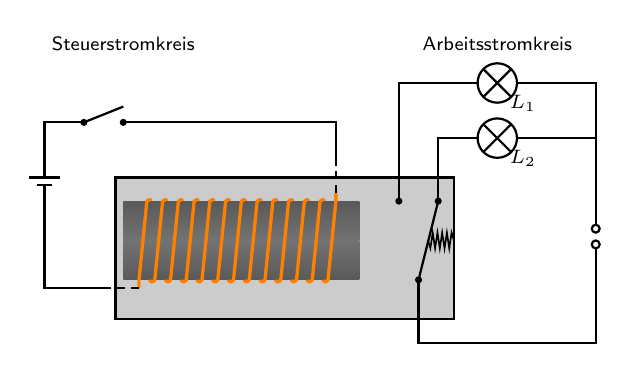
\begin{tikzpicture}
		% Kasten für Relais
		\draw [thick,fill=gray!40] (-0.1,-0.5) rectangle (4.2,1.3);
		%Eisenkern
		\shade [top color=gray!70!black, bottom color=gray!90!black] (0,0.5) rectangle (3,1);
		\shade [bottom color=gray!70!black, top color=gray!90!black] (0,0) rectangle (3,0.5);
		% Spule
		%Anfangspunkt (0.2,-0.1)
		\draw [color=orange, very thick] (0.2,-0.1) -- (0.2,0) -- ++(0.1,1) .. controls ++(0.05,0.04) and ++(0,0) .. ++(0.05,0);
		\foreach \x in {0.4,0.6,...,2.6} {
			\draw [color=orange, very thick] (\x-0.06,0) -- (\x-0.06,-0.01) .. controls ++(0.03,-0.04) and ++(0,0) .. (\x,0) -- ++(0.1,1) .. controls ++(0.05,0.04) and ++(0,0) .. ++(0.05,0);
		}
		\draw [color=orange, very thick] (2.6-0.06,0) -- (2.6-0.06,-0.01) .. controls ++(0.03,-0.04) and ++(0,0) .. (2.6,0) -- ++(0.1,1) -- ++(0,0.1);  % Endpunkt: (2.7,1.1)
		%%%% Steuerstromkreis
		\draw (2.7,1.1) [densely dashed, thick] -- (2.7,1.5);
		\draw [thick] (2.7,1.5) -- (2.7,2) -- (0,2);
		%Schalter offen
		\draw [thick,fill=black] (0,2) circle [radius=0.03]; 
		\draw [thick] (-0.5,2) -- ++ (0.5,0.2);
		\draw [thick,fill=black] (-0.5,2) circle [radius=0.03]; 
		\draw [thick] (-0.5,2) -- (-1,2) -- (-1,1.3) ++(-0.2,0) -- ++(0.4,0) ++(-0.1,-0.1) -- ++(-0.2,0) ++(0.1,0) -- (-1,-0.1) -- (-0.2,-0.1);
		\draw [thick,densely dashed] (0.2,-0.1) -- (-0.2,-0.1);
		%%%% Arbeitsstromkreis
		%Wechselschalter
		\draw [thick, fill=black] (3.75,0) circle [radius=0.03];
		\draw [thick, fill=black] (3.5,1) circle [radius=0.03];
		\draw [thick, fill=black] (4,1) circle [radius=0.03];
		\draw [thick] (3.75,0) -- (4,1);
		%Feder
		\draw [semithick] (4.2,0.5) -- ++(-0.03,0.1) -- ++(-0.03,-0.2) -- ++(-0.03,0.2) -- ++(-0.03,-0.2) -- ++(-0.03,0.2) -- ++(-0.03,-0.2)-- ++(-0.03,0.2) -- ++(-0.03,-0.2)-- ++(-0.03,0.2) -- ++(-0.03,-0.2) -- ++(-0.03,0.1);
		% Stromkreis an sich
		\draw [thick] (3.75,0) -- (3.75,-0.8) -- (6,-0.8) -- (6,0.4);
		\draw [thick] (6,0.45) circle [radius=0.05];
		\draw [thick] (4,1) -- (4,1.8) -- (4.5,1.8);
		\draw [thick] (4.75,1.8) circle [radius=0.25] node [below right =0.8] {\scriptsize\sffamily $L_2$};
		\draw [thick] (4.75,1.8) -- ++(45:0.25);
		\draw [thick] (4.75,1.8) -- ++(135:0.25);
		\draw [thick] (4.75,1.8) -- ++(225:0.25);
		\draw [thick] (4.75,1.8) -- ++(315:0.25);
		\draw [thick] (5,1.8) -- (6,1.8) -- (6,0.7);
		\draw [thick] (6,0.65) circle [radius=0.05];
		\draw [thick] (3.5,1) -- (3.5,2.5) -- (4.5,2.5);
		\draw [thick] (4.75,2.5) circle [radius=0.25] node [below right =0.8] {\scriptsize\sffamily $L_1$};
		\draw [thick] (4.75,2.5) -- ++(45:0.25);
		\draw [thick] (4.75,2.5) -- ++(135:0.25);
		\draw [thick] (4.75,2.5) -- ++(225:0.25);
		\draw [thick] (4.75,2.5) -- ++(315:0.25);
		\draw [thick] (5,2.5) -- (6,2.5) -- (6,1.8);
		% Bezeichnungen
		\node at (0,3) {\scriptsize\sffamily Steuerstromkreis};
		\node at (4.75,3) {\scriptsize\sffamily Arbeitsstromkreis};
		\end{tikzpicture}
		\caption{Aufbau eines Relais (grau unterlegt) einschließlich der Stellung des Wechselschalters, wenn im Steuerstromkreis kein Strom fließt.}
	\end{figure}
\end{minipage}
\hfill
\begin{minipage}{0.48\textwidth}
	\begin{figure}[H]
		\centering
		%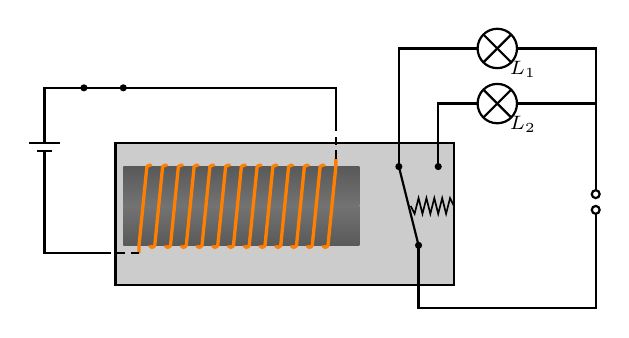
\begin{tikzpicture}
	% Kasten für Relais
	\draw [thick,fill=gray!40] (-0.1,-0.5) rectangle (4.2,1.3);
	%Eisenkern
	\shade [top color=gray!70!black, bottom color=gray!90!black] (0,0.5) rectangle (3,1);
	\shade [bottom color=gray!70!black, top color=gray!90!black] (0,0) rectangle (3,0.5);
	% Spule
	%Anfangspunkt (0.2,-0.1)
	\draw [color=orange, very thick] (0.2,-0.1) -- (0.2,0) -- ++(0.1,1) .. controls ++(0.05,0.04) and ++(0,0) .. ++(0.05,0);
	\foreach \x in {0.4,0.6,...,2.6} {
		\draw [color=orange, very thick] (\x-0.06,0) -- (\x-0.06,-0.01) .. controls ++(0.03,-0.04) and ++(0,0) .. (\x,0) -- ++(0.1,1) .. controls ++(0.05,0.04) and ++(0,0) .. ++(0.05,0);
	}
	\draw [color=orange, very thick] (2.6-0.06,0) -- (2.6-0.06,-0.01) .. controls ++(0.03,-0.04) and ++(0,0) .. (2.6,0) -- ++(0.1,1) -- ++(0,0.1);  % Endpunkt: (2.7,1.1)
	%%%% Steuerstromkreis
	\draw (2.7,1.1) [densely dashed, thick] -- (2.7,1.5);
	\draw [thick] (2.7,1.5) -- (2.7,2) -- (0,2);
	%Schalter geschlossen
	\draw [thick,fill=black] (0,2) circle [radius=0.03]; 
	\draw [thick] (-0.5,2) -- ++ (0.5,0);
	\draw [thick,fill=black] (-0.5,2) circle [radius=0.03]; 
	\draw [thick] (-0.5,2) -- (-1,2) -- (-1,1.3) ++(-0.2,0) -- ++(0.4,0) ++(-0.1,-0.1) -- ++(-0.2,0) ++(0.1,0) -- (-1,-0.1) -- (-0.2,-0.1);
	\draw [thick,densely dashed] (0.2,-0.1) -- (-0.2,-0.1);
	%%%% Arbeitsstromkreis
	%Wechselschalter
	\draw [thick, fill=black] (3.75,0) circle [radius=0.03];
	\draw [thick, fill=black] (3.5,1) circle [radius=0.03];
	\draw [thick, fill=black] (4,1) circle [radius=0.03];
	\draw [thick] (3.75,0) -- (3.5,1);
	%Feder
	\draw [semithick] (4.2,0.5) -- ++(-0.05,0.1) -- ++(-0.05,-0.2) -- ++(-0.05,0.2) -- ++(-0.05,-0.2) -- ++(-0.05,0.2) -- ++(-0.05,-0.2)-- ++(-0.05,0.2) -- ++(-0.05,-0.2)-- ++(-0.05,0.2) -- ++(-0.05,-0.2) -- ++(-0.05,0.1);
	% Stromkreis an sich
	\draw [thick] (3.75,0) -- (3.75,-0.8) -- (6,-0.8) -- (6,0.4);
	\draw [thick] (6,0.45) circle [radius=0.05];
	\draw [thick] (4,1) -- (4,1.8) -- (4.5,1.8);
	%Lampe L2
	\draw [thick] (4.75,1.8) circle [radius=0.25] node [below right =0.8] {\scriptsize $L_2$};
	\draw [thick] (4.75,1.8) -- ++(45:0.25);
	\draw [thick] (4.75,1.8) -- ++(135:0.25);
	\draw [thick] (4.75,1.8) -- ++(225:0.25);
	\draw [thick] (4.75,1.8) -- ++(315:0.25);
	%weiter mit Kabels
	\draw [thick] (5,1.8) -- (6,1.8) -- (6,0.7);
	\draw [thick] (6,0.65) circle [radius=0.05];
	\draw [thick] (3.5,1) -- (3.5,2.5) -- (4.5,2.5);
	%Lampe L1
	\draw [thick] (4.75,2.5) circle [radius=0.25] node [below right =0.8] {\scriptsize $L_1$};
	\draw [thick] (4.75,2.5) -- ++(45:0.25);
	\draw [thick] (4.75,2.5) -- ++(135:0.25);
	\draw [thick] (4.75,2.5) -- ++(225:0.25);
	\draw [thick] (4.75,2.5) -- ++(315:0.25);
	% Kabels
	\draw [thick] (5,2.5) -- (6,2.5) -- (6,1.8);
\end{tikzpicture}
		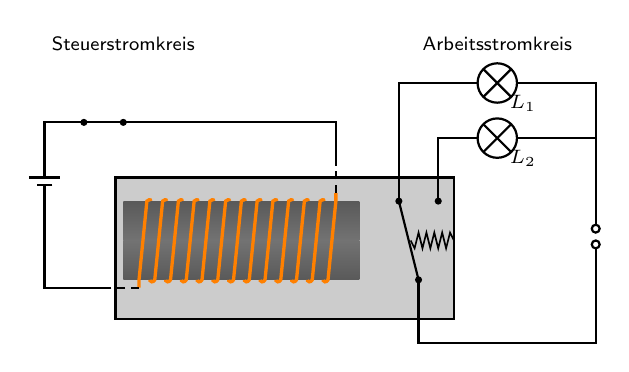
\begin{tikzpicture}
		% Kasten für Relais
		\draw [thick,fill=gray!40] (-0.1,-0.5) rectangle (4.2,1.3);
		%Eisenkern
		\shade [top color=gray!70!black, bottom color=gray!90!black] (0,0.5) rectangle (3,1);
		\shade [bottom color=gray!70!black, top color=gray!90!black] (0,0) rectangle (3,0.5);
		% Spule
		%Anfangspunkt (0.2,-0.1)
		\draw [color=orange, very thick] (0.2,-0.1) -- (0.2,0) -- ++(0.1,1) .. controls ++(0.05,0.04) and ++(0,0) .. ++(0.05,0);
		\foreach \x in {0.4,0.6,...,2.6} {
			\draw [color=orange, very thick] (\x-0.06,0) -- (\x-0.06,-0.01) .. controls ++(0.03,-0.04) and ++(0,0) .. (\x,0) -- ++(0.1,1) .. controls ++(0.05,0.04) and ++(0,0) .. ++(0.05,0);
		}
		\draw [color=orange, very thick] (2.6-0.06,0) -- (2.6-0.06,-0.01) .. controls ++(0.03,-0.04) and ++(0,0) .. (2.6,0) -- ++(0.1,1) -- ++(0,0.1);  % Endpunkt: (2.7,1.1)
		%%%% Steuerstromkreis
		\draw (2.7,1.1) [densely dashed, thick] -- (2.7,1.5);
		\draw [thick] (2.7,1.5) -- (2.7,2) -- (0,2);
		%Schalter geschlossen
		\draw [thick,fill=black] (0,2) circle [radius=0.03]; 
		\draw [thick] (-0.5,2) -- ++ (0.5,0);
		\draw [thick,fill=black] (-0.5,2) circle [radius=0.03]; 
		\draw [thick] (-0.5,2) -- (-1,2) -- (-1,1.3) ++(-0.2,0) -- ++(0.4,0) ++(-0.1,-0.1) -- ++(-0.2,0) ++(0.1,0) -- (-1,-0.1) -- (-0.2,-0.1);
		\draw [thick,densely dashed] (0.2,-0.1) -- (-0.2,-0.1);
		%%%% Arbeitsstromkreis
		%Wechselschalter
		\draw [thick, fill=black] (3.75,0) circle [radius=0.03];
		\draw [thick, fill=black] (3.5,1) circle [radius=0.03];
		\draw [thick, fill=black] (4,1) circle [radius=0.03];
		\draw [thick] (3.75,0) -- (3.5,1);
		%Feder
		\draw [semithick] (4.2,0.5) -- ++(-0.05,0.1) -- ++(-0.05,-0.2) -- ++(-0.05,0.2) -- ++(-0.05,-0.2) -- ++(-0.05,0.2) -- ++(-0.05,-0.2)-- ++(-0.05,0.2) -- ++(-0.05,-0.2)-- ++(-0.05,0.2) -- ++(-0.05,-0.2) -- ++(-0.05,0.1);
		% Stromkreis an sich
		\draw [thick] (3.75,0) -- (3.75,-0.8) -- (6,-0.8) -- (6,0.4);
		\draw [thick] (6,0.45) circle [radius=0.05];
		\draw [thick] (4,1) -- (4,1.8) -- (4.5,1.8);
		%Lampe L2
		\draw [thick] (4.75,1.8) circle [radius=0.25] node [below right =0.8] {\scriptsize\sffamily $L_2$};
		\draw [thick] (4.75,1.8) -- ++(45:0.25);
		\draw [thick] (4.75,1.8) -- ++(135:0.25);
		\draw [thick] (4.75,1.8) -- ++(225:0.25);
		\draw [thick] (4.75,1.8) -- ++(315:0.25);
		%weiter mit Kabels
		\draw [thick] (5,1.8) -- (6,1.8) -- (6,0.7);
		\draw [thick] (6,0.65) circle [radius=0.05];
		\draw [thick] (3.5,1) -- (3.5,2.5) -- (4.5,2.5);
		%Lampe L1
		\draw [thick] (4.75,2.5) circle [radius=0.25] node [below right =0.8] {\scriptsize\sffamily $L_1$};
		\draw [thick] (4.75,2.5) -- ++(45:0.25);
		\draw [thick] (4.75,2.5) -- ++(135:0.25);
		\draw [thick] (4.75,2.5) -- ++(225:0.25);
		\draw [thick] (4.75,2.5) -- ++(315:0.25);
		% Kabels
		\draw [thick] (5,2.5) -- (6,2.5) -- (6,1.8);
		% Bezeichnungen
		\node at (0,3) {\scriptsize\sffamily Steuerstromkreis};
		\node at (4.75,3) {\scriptsize\sffamily Arbeitsstromkreis};
		\end{tikzpicture}
		\caption{Aufbau eines Relais (grau unterlegt) einschließlich der Stellung des Wechselschalters, wenn im Steuerstromkreis Strom fließt.}
	\end{figure}
\end{minipage}

\bigskip
\begin{aufgabe}\emph{Physikalischer Hintergrund zum Relais}
	
	Erkläre die Stellung des Wechselschalters in Abhängigkeit des Steuerstromkreises in den beiden abgebildeten Situationen. Welche Lampe leuchtet?
	
	Die Kontakte am Wechselschalter werden mit \emph{NO} (\emph{normally open}), \emph{NC} (\emph{normally closed}) und \emph{C} (\emph{common ground}) bezeichnet. Ordne die Bezeichnungen den Kontakten in der Skizze zu.
\end{aufgabe}

\begin{aufgabe}\emph{Anschluss eines Relais}
	
	\begin{wrapfigure}{r}{0.3\textwidth}
		\vspace{-\baselineskip}
		\centering
		\includegraphics[width=0.17\textwidth]{./pics/relais-klein.png}
	\end{wrapfigure}
	\textbf{a)} Wie aus dem obigen Schaltplan ersichtlich wird, hat ein Relais fünf Anschlüsse, die jedoch nicht beschriftet sind. Suche im Internet nach \enquote{Datasheet <Gerätebezeichnung des Relais>} (Bezeichnung vom Relais ablesen) und entnimm dem Datenblatt, welche Anschlüsse zum Steuer- bzw. Arbeitsstromkreis gehören.
	
	\medskip
	\ausrufezeichen \textbf{Achtung:} Auf dem Relais ist angegeben, dass damit bis zu $\SI{250}{\volt}$ Wechselspannung und $\SI{10}{\ampere}$ geschaltet werden können. Das sollte man mit solch billigen Bastelmodulen aber \textbf{niemals machen}! Generell gilt: \textbf{Nur ausgebildete Fachleute sollten mit Spannungen von mehr als 24\,V hantieren!}
	
	\bigskip
	\begin{minipage}{0.44\textwidth}
		\textbf{b)} Baue die Schaltung entsprechend des rechts abgebildeten Schaltplans auf. Nutze dazu das \enquote{Power Module} auf dem Steckbrett (Erklärung unten). Probiere die Schaltung des Relais aus, indem du die Stromzufuhr der Spule unterbrichst und wieder herstellst.
	\end{minipage}
	\hfill
	\begin{minipage}{0.54\textwidth}
		\centering
		\includegraphics[width=\textwidth]{./Zeichnungen/relais-schaltung-ohne-arduino.png}
	\end{minipage}
	
	\medskip
	\textbf{c)} Ordne in einer Skizze des Relais die Anschlüsse ihrer Bezeichnung (A1, A2, C, NO, NC) zu.
\end{aufgabe}
% Erklärung der Pins des Relais + Ausprobieren der NC-Verbindung und NO-Verbindung mit LED+Vorwiderstand -> in Skizze festhalten, wo NC und wo NO ist

\bigskip
\begin{zsfg}{Das \enquote{Power Supply Module}}\label{powersupplymodule}
	
	\begin{wrapfigure}{r}{0.37\textwidth}
		\vspace{-0.5\baselineskip}
		\centering
		\includegraphics[width=0.35\textwidth]{./pics/steckbrett-mit-power-module-klein.png}
		\vspace{-\baselineskip}
	\end{wrapfigure}
	Das Power Supply Module dient zur Spannungsversorgung auf einem Steckbrett. Dazu kann eine Batterie mit $\SI{6,5}{\volt}$ bis $\SI{12}{\volt}$ oder ein USB-Kabel angeschlossen werden. Die Spannung wird auf dem Modul je nach Einstellung der \emph{Jumper} auf $\SI{5}{\volt}$ oder $\SI{3,3}{\volt}$ heruntergeregelt. Dazu verbindet man mithilfe der Jumper die Anschlüsse \texttt{5V} und \texttt{OFF} bzw. \texttt{3.3} und \texttt{OFF}.
	
	Die Spannung kann entlang der langen äußeren Leisten abgegriffen werden, wenn der Taster neben der Hohlbuchse gedrückt ist. Die Zuordnung zu Pluspol und Minuspol ist auf dem Power Supply Module mit \texttt{+} bzw. \texttt{-} markiert.
\end{zsfg}
% Gefahrenhinweis!
% Erklärung des Steuerstromkreises mit Transistor und Diode
% Aufgabe: Aufbauen und ausprobieren

\newpage
\begin{aufgabe}\emph{Anschluss eines Relais am Arduino}
	\vspace{-0.5\baselineskip}
	\begin{figure}[H]
		\centering
		\includegraphics[width=0.65\textwidth]{./Zeichnungen/relais-schaltung-mit-arduino.png}
	\end{figure}
	\vspace{-0.5\baselineskip}
	\marginpar{%
		\scriptsize
		\centering
		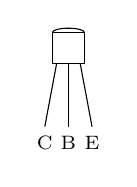
\begin{tikzpicture}
		\draw (-0.2,0.8) rectangle (0.2,1.2);
		\draw (0.2,1.2) arc [start angle=0,end angle=180,x radius=0.2,y radius=0.05];
		\draw (-0.15,0.8) -- (-0.3,0) node [below] {\scriptsize C};
		\draw (0,0.8) -- (0,0) node [below] {\scriptsize B};
		\draw (0.15,0.8) -- (0.3,0) node [below] {\scriptsize E};
		\end{tikzpicture}
		
		npn-Transistor; Blick auf flache Seite
	}
	Der Schaltplan oben zeigt, wie man ein Relais mit dem Arduino steuert.
	\begin{enumerate}[itemsep=0mm, parsep=0mm, label=\alph*)]
		\item Erkläre die Funktion der in Sperrrichtung geschalteten Diode parallel zur Spule des Relais.
		\item Erkläre die Funktion des Transistors.
		
		\emph{Hinweis:} Der 5V-Pin und der GND-Pin vertragen bis zu $\SI{200}{\milli\ampere}$. Die Digitalpins vertragen dagegen maximal $\SI{40}{\milli\ampere}$; normalerweise sollten $\SI{20}{\milli\ampere}$ nicht überschritten werden (s. \href{https://playground.arduino.cc/Main/ArduinoPinCurrentLimitations/}{Pin Current Limitations}).
		\item Baue die Schaltung auf und teste sie mit einem Blink-Programm.
	\end{enumerate}
\end{aufgabe}

% E-Motor anschließen
\begin{projekt}[Waschmaschinensteuerung]\label{proj:waschmaschinensteuerung}
	\begin{figure}[H]
		\centering
		\includegraphics[width=0.7\textwidth]{./Zeichnungen/relais-schaltung-mit-motor.png}
	\end{figure}
	Baue die oben abgebildete Schaltung zur Steuerung eines Elektromotors mit einem Relais am Arduino auf. Achte auf die in Sperrrichtung geschaltete Diode parallel zum Motor.
	
	Schließe dann drei Taster an (mit Widerstand! - vgl. Abschnitt \ref{sec:elektrisches-potential}).
	
	\emph{Programmiere nun einen einfachen steuerbaren Waschmaschinenprototypen!}
	
	Dieser gibt solange auf dem seriellen Monitor die aktuell gesetzte Waschzeit aus, bis der mittlere Taster gedrückt wurde, was bedeutet, dass der Waschvorgang startet (der Motor dreht sich für die angegebene Zeit). Wenn der linke Taster gedrückt wird, wird die Waschzeit verringert (aber nicht niedriger als eine Sekunde). Wenn der rechte Taster gedrückt wird, wird die Waschzeit vergrößert (aber nicht größer als 30 Sekunden). Nach dem Waschen fragt der Waschmaschinenprototyp wieder nach der Waschzeit.
\end{projekt}

\begin{recherche}{Anwendungen von Relais}
	Recherchiere einige Anwendungen von Relais. Einen guten Startpunkt bietet die \href{https://www.leifiphysik.de/elektrizitaetslehre/elektromagnetismus/ausblick/relais}{Seite von Leifiphysik}.
\end{recherche}
% Recherchiere Anwendungen von Relais-Schaltungen, z. B. bei Leifiphysik

\begin{aufgabe} \emph{Vergleich von Transistor und Relais}
	
	Transistoren und Relais erfüllen im Wesentlichen die gleiche Funktion: Sie sind elektronisch steuerbare Schalter, bei denen die zu steuernde Stromstärke größer sein kann als die Stromstärke im Steuerstromkreis. Dennoch gibt es einige Unterschiede, weshalb sie für unterschiedliche Aufgaben geeignet sind.
	
	Vergleiche die Steuerung mit einem Transistor und mit einem Relais hinsichtlich der Vor- und Nachteile.
\end{aufgabe}
% Vergleiche die Steuerung mit einem Transistor und mit einem Relais im Hinblick auf die jeweiligen Vor- und Nachteile.

\bigskip
\begin{zsfg}{Relais}
		\begin{wrapfigure}{r}{0.45\textwidth}
		\vspace{-0.3\baselineskip}
		\centering
		\hfill
		\includegraphics[width=0.21\textwidth]{./pics/relais-klein.png}
		\hfill
		\includegraphics[width=0.21\textwidth]{./Zeichnungen/schaltsymbol-relais.png}
		\hfill
		\caption{Relais in real und als Schaltsymbol.}
	\end{wrapfigure}
	Relais sind elektronisch steuerbare Wechselschalter, bei denen Steuerstromkreis und Arbeitsstromkreis komplett voneinander getrennt sind. Im Steuerstromkreis ist eine Spule, die ein Magnetfeld aufbaut, wenn der Strom eingeschaltet wird. Dadurch wird ein Wechselschalter im Arbeitsstromkreis angezogen, sodass er seine Position wechselt und einen anderen Teil des Arbeitsstromkreises anschaltet. Wenn der Strom durch die Spule im Steuerstromkreis abgeschaltet wird, baut sich das Magnetfeld ab und der Wechselschalter im Arbeitsstromkreis wird durch eine Feder zurück in die Standardstellung (NC) gezogen, sodass der erste Teil des Arbeitsstromkreises angeschaltet wird.
	
	Die Anschlüsse der Spule werden in der Regel mit \emph{A1} und \emph{A2} bezeichnet; die Anschlüsse am Wechselschalter mit \emph{NO} (\emph{normally open}), \emph{NC} (\emph{normally closed}) und \emph{C} (\emph{common ground}) bezeichnet.
\end{zsfg}

\newpage
\subsection{Elektromotoren mit dem Motortreiber-IC L293D steuern (inkl. Drehrichtung)}

Die Steuerung von Motoren erfordert in den oben beschriebenen Fällen stets mehrere Bauteile und einige Überlegungen zum Aufbau der Schaltung. Außerdem kann dabei nicht die Drehrichtung geändert werden. Der integrierte Schaltkreis L293D vereinfacht den Aufbau der Schaltung für gleich zwei Motoren und ermöglicht zusätzlich die flexible Steuerung der Drehrichtung.

\begin{ziel}
	\textbf{Frage:} Wie steuert man einen Motor mit dem L293D? 
\end{ziel}

% Aufbau des IC - Vierquadrantensteller
\begin{aufgabe} \emph{Aufbau des L293D - der Vierquadrantensteller}
	
	Um die Drehrichtung des Motors kontrollieren zu können, braucht man eine spezielle Anordnung von Transistoren, die als \emph{H-Brücke} oder \emph{Vierquadrantensteller} bezeichnet wird. Dieser Aufbau befindet sich auch im L293D.
	
	\begin{figure}[H]
		\centering
		\includegraphics[width=0.8\textwidth]{./Zeichnungen/vierquadrantensteller.png}
		\caption{Vereinfachter Aufbau eines Vierquadrantenstellers mit Transistoren und zugehörigen Freilaufdioden (links) sowie die noch einmal vereinfachte Ersatzschaltung mit Schaltern.}
	\end{figure}
	
	\begin{enumerate}[label=\alph*), itemsep=0mm, parsep=0mm]
		\item Die Drehrichtung des Motors hängt davon ab, in welcher Richtung der Strom durch den Motor fließt. Notiere, welche Transistoren\,/\,Schalter eingeschaltet und welche Transistoren\,/\,Schalter ausgeschaltet sein müssen, damit der Strom von links nach rechts durch den Motor fließt. Notiere danach die Kombination für die Stromrichtung von rechts nach links.
		\item Erkläre, wie sich der Motor mithilfe der vier Transistoren bzw. Schalter bremsen lässt.
		\item Welche Schaltkombinationen der Transistoren müssen unbedingt vermieden werden?
	\end{enumerate}
	
	\emph{Hinweis:} Die Freilaufdioden dienen dazu, die vom Motor induzierten Ströme abfließen zu lassen.
\end{aufgabe}

Da stets zwei Transistoren gemeinsam eingeschaltet werden müssen, könnten diese beim Anschluss an den Arduino über einen gemeinsamen Digitalpin gesteuert werden. Zudem ist es im Allgemeinen sinnvoll, für den Motor und den Arduino verschiedene Spannungsquellen zu verwenden, die über einen gemeinsamen GND-Anschluss geerdet werden, damit die möglicherweise hohen Ströme des Motors den Arduino nicht zerstören.

\begin{figure}[H]
	\centering
	\includegraphics[width=0.8\textwidth]{./Zeichnungen/vierquadrantensteller-an-arduino.png}
	\caption{Steuerung eines Motors mit einem Vierquadrantensteller am Arduino.}
\end{figure}

Bei der oben dargestellten Schaltung muss jedoch immer noch genau darauf geachtet werden, dass nicht versehentlich alle vier Transitoren leitend geschaltet werden. Daher ist die Steuerung mit dem L293D noch ein wenig komplexer - die oben angestellten Überlegungen verdeutlichen aber gut den prinzipiellen Aufbau.

\begin{zsfg}{Der Motortreiber L293D}
	
	\medskip
	\begin{minipage}{0.7\textwidth}
		Der L293D ist ein integrierter Schaltkreis (\emph{IC} von engl. \emph{integrated circuit}), das heißt, in das schwarze Gehäuse sind Schaltkreise mit Transistoren, Widerständen, Dioden etc. integriert. Genauer gesagt, enthält der L293D zwei H-Brücken oder Vierquadrantensteller, die sich mit den Pins an beiden Seiten steuern lassen. Bei der Nummerierung der Pins ist darauf zu achten, dass die kleine Kerbe nach oben gehalten wird.
	\end{minipage}
	\hfill
	\begin{minipage}{0.28\textwidth}
		\begin{minipage}{0.48\textwidth}
			\centering
			\includegraphics[width=0.8\textwidth]{./pics/l293d.jpg}
		\end{minipage}
		\hfill
		\begin{minipage}{0.48\textwidth}
			\centering
			\includegraphics[width=\textwidth]{./Zeichnungen/motortreiber-l293d.png}
		\end{minipage}
	\end{minipage}
	
	\medskip		
	\emph{Achtung: Der L293D kann leicht mit anderen Bauteilen wie z.\,B. einem Shift-Register verwechselt werden, das dieselbe Bauart hat. Um sicher zu gehen, muss man die winzige Beschriftung des Bauteils lesen!}
\end{zsfg}

Im Folgenden wird die Belegung der Pins für die linke Seite beschrieben (vgl. Abbildung \ref{abb:l293d-an-arduino}). Die Belegung auf der rechten Seite verläuft analog.

Der Motor wird an Pin 3 und 6 (\texttt{Out1} und \texttt{Out2}) angeschlossen. Der jeweilige Zustand der \texttt{Out}-Pins kann über Pin 2 und 7 (\texttt{In1} und \texttt{In2}) geregelt werden. Wenn an \texttt{In1} der Zustand \texttt{HIGH} und an \texttt{In2} \texttt{LOW} anliegt, wird das auf \texttt{Out1} und \texttt{Out2} übertragen, sodass durch den Motor ein Strom fließen kann. Diese Übertragung wird jedoch durch Pin 1 (\texttt{En1,2} für \emph{enable pin 1, 2}) gesteuert. Wenn an \texttt{En1,2} \texttt{HIGH} anliegt, wird die Input-Konfiguration übertragen, bei \texttt{LOW} nicht. Durch ein PWM-Signal an \texttt{En1,2} kann die Leistung des Motors entsprechend gedrosselt werden.

Die vier \texttt{GND}-Anschlüsse dienen zur Stromversorgung und zur Wärmeableitung, falls hohe Ströme auftreten. An \texttt{Vmotor} wird der Pluspol der Versorgungsspannung für den Motor angeschlossen; an \texttt{Vcc} der Logik-Pegel von 5V für die Schaltung des IC.

\begin{figure}[H]
	\centering
	\includegraphics[width=0.5\textwidth]{./Zeichnungen/l293d-an-arduino.png}
	\caption{Steuerung eines Motors mit dem L293D.}
	\label{abb:l293d-an-arduino}
\end{figure}

% Pin-Belegung des IC

\begin{aufgabe} \emph{Betrieb des L293D}
	
	\medskip
	\begin{minipage}{0.43\textwidth}
		\begin{enumerate}[label=\alph*), itemsep=0mm, parsep=0mm]
			\item Baue die oben beschriebene Schaltung auf. Nutze dazu das \emph{Power Supply Module} (siehe S. \pageref{powersupplymodule}).
			\item Experimentiere mit verschiedenen Input-Konfigurationen und PWM-Werten für den \texttt{En1,2}-Pin. 
			
			\item Halte die Wirkung auf den Motor tabellarisch fest. Hier genügt es, wenn für den \texttt{En1,2}-Pin nur zwischen \emph{ein / 1} und \emph{aus / 0} unterschieden wird.
			
			\begin{tabular}{c|c|c|c}
				In1 & In 2 & En1,2 & Wirkung \\ \hline
				1 & 0 & 1 & \dots \\
			\end{tabular}
		\end{enumerate}
	\end{minipage}
	\hfill
	\begin{minipage}{0.55\textwidth}
		\begin{figure}[H]
			\centering
			\includegraphics[width=0.9\textwidth]{./pics/prog-konfiguration-l293d.png}
			\includegraphics[width=0.9\textwidth]{./pics/prog-motorsteuerung-l293d.png}
		\end{figure}
	\end{minipage}
\end{aufgabe}
% Anschluss am Arduino und Aufbau der Schaltung sowie Test mit einfachem Programm
% Aufgabe: Alle Kombinationen durchprobieren und tabellarisch festhalten

\begin{recherche}{Wie stark darf der L293D belastet werden?}
	Bei Motoren ist immer genau darauf zu achten, welche Stromstärken und Spannungen die verwendeten Bauteile aushalten. Suche nach dem Datenblatt (\emph{data sheet}) des L293D und notiere die Maximalwerte zu Versorgungsspannung, Stromstärke und kurzfristige Spitzenstromstärke, die der IC aushält (\emph{absolute maximum ratings}). 
\end{recherche}
% Recherche: Absolute maximum ratings

%TODO: Funktionen zur Motorsteuerung erstellen

\section{Vermischte Übungen}

\begin{aufgabe} \emph{Reihenschaltung}
	
	Eine rote LED soll an Pin 13 des Arduino betrieben werden. Durch die LED soll eine Stromstärke von $\SI{10}{\milli\ampere}$ fließen, was bei einer Spannung von $\SI{2,1}{\volt}$ an der LED der Fall ist. 
	\begin{enumerate}[label=\alph*), itemsep=0ex]
		\item Zeichne den zugehörigen Schaltplan.
		\item Berechne, wie groß der Vorwiderstand gewählt werden muss, damit diese Werte erreicht werden.
	\end{enumerate}
\end{aufgabe}

\begin{aufgabe} \emph{Parallelschaltung}
	
	Drei grüne LEDs sollen parallel geschaltet an Pin 13 des Arduino angeschlossen und mit einem gemeinsamen Vorwiderstand betrieben werden. Die LEDs halten eine Stromstärke von maximal $\SI{20}{\milli\ampere}$ bei einer Spannung von $\SI{3,3}{\volt}$ aus.
	
	\begin{enumerate}[label=\alph*), itemsep=0ex]
		\item Zeichne den zugehörigen Schaltplan.
		\item Ein Digitalpin am Arduino darf maximal mit einer Stromstärke von $\SI{40}{\milli\ampere}$ belastet werden. Berechne, welche Stromstärke dann maximal durch die einzelnen LEDs fließen darf.
		\item Der Tabelle unten kannst du den zugehörigen Spannungswert an den LEDs entnehmen. Berechne, wie groß der gemeinsame Vorwiderstand der LEDs sein muss, damit die in b) berechnete Stromstärke eingehalten wird.
		
		\begin{tabular}{c | c | c | c | c | c | c}
			\hline
			\textbf{Spannung U} & 3,03\,V & 3,07\,V & 3,1\,V & 3,13\,V & 3,16\,V & 3,19\,V \\ \hline
			\textbf{Stromstärke I} & 10\,mA & 11\,mA & 12\,mA & 13\,mA & 14\,mA & 15\,mA  \\ \hline
		\end{tabular}
	\end{enumerate}
\end{aufgabe}

\begin{aufgabe} \emph{Schaltung einer RGB-LED}
	
	\begin{wrapfigure}{r}{0.3\textwidth}
		\vspace{-\baselineskip}
		\centering
		\includegraphics[width=0.2\textwidth]{./pics/rgb-led-schaltplan.png}
		\caption{Verschaltung der RGB-LED.}
		\vspace{-\baselineskip}
	\end{wrapfigure}
	Eine RGB-LED besteht aus drei einzelnen LEDs (rot, grün, blau), die jeweils über einen eigenen Digitalpin angesteuert werden (vgl. Schaltplan rechts). Am gemeinsamen GND-Anschluss soll ein gemeinsamer Vorwiderstand für alle LEDs angebracht werden, um die Stromstärke auf maximal $\SI{15}{\milli\ampere}$ zu begrenzen. Die Spannung an den LEDs sollte dann $\SI{2,25}{\volt}$ nicht überschreiten.
	\begin{enumerate}[label=\alph*), itemsep=0ex]
		\item Erkläre, welche Unterschiede zur Parallelschaltung von drei LEDs an \emph{einem} Digitalpin zu beachten sind.
		\item Berechne, wie groß der gemeinsame Vorwiderstand mindestens sein muss.
	\end{enumerate}
\end{aufgabe}

\newpage
\section{Ausblick}\label{sec:ausblick-elektrik}

\begin{ziel}
	\textbf{Offene Fragen:}
	
	\begin{itemize}[itemsep=0ex,parsep=0ex]
		\item Wie werden weitere Bauteile angeschlossen und im Programm angesprochen?
		\item Wie wird die Programmlogik physikalisch abgebildet? %-> Logikgatter [am Ende von Kap. Elektrik]
		\item Wie funktionieren solche Bauteile wie LDR, NTC, Dioden, Transistoren?
	\end{itemize}
\end{ziel}

\vfill
\begin{links}
	\item \href{https://www.instructables.com/id/Arduino-UNO-Laser-Game/}{Laser-Game}
	
	Ein kleines Spiel, das sich auf einfache Weise nachbauen lässt.
	
	\item \href{https://www.youtube.com/watch?v=O_Q1WKCtWiA}{Arduino Garden Controller}
	
	Gartenarbeit muss heute nicht mehr aufwendig sein: Mit einem Arduino lassen sich die Pflanzen automatisch bewässern, wenn die Erde nicht mehr feucht genug ist. Die erhobenen Daten lassen sich außerdem schön visualisieren.
	
	\item \href{https://www.youtube.com/watch?v=at7wmm9t8UE}{Wetterstation von bitluni}
	
	\href{https://www.youtube.com/watch?v=aHkec8bA8iI}{Das Problem mit Wettervorhersagen (\emph{Dr. Whatson}, Youtube)}
	
	Selbst gebaute Wetterstationen sind beliebte Anfängerprojekte, bei denen meist ein WLAN-fähiger Mikrocontroller auf Basis des ESP8266 zum Einsatz kommt. Dieser lässt sich ebenfalls über die Arduino IDE programmieren. Wer etwas mehr Hintergrundwissen dazu haben will, schaut sich das Video von \emph{Dr. Whatson} an, der außerdem das Projekt \href{https://www.sensebox.de/}{SenseBox} vorstellt.
	
	\item \href{https://www.youtube.com/watch?v=KtSCo6hIlRQ}{\enquote{Use the force or your brainwaves} (Youtube)}
	
	\href{https://create.arduino.cc/projecthub/Imetomi/use-the-force-or-your-brainwaves-9e839b}{\enquote{Use the force or your brainwaves} (Projektseite)}
	
	Der Schüler Imets Tamás hat es mithilfe mehrerer Arduinos geschafft, seine Gehirnwellen einzulesen und zu nutzen, um einen Roboter zu steuern!

	\item \href{https://www.instructables.com/id/Self-Driving-Car-Using-Arduinoautonomous-Guided-Ve/}{Autonomes Auto}
	
	Der Bastler hinter diesem Projekt hat einen Arduino-basierten Prototypen für ein autonomes Auto entworfen.
	
	\item \href{https://www.instructables.com/id/Arduino-Controlled-Game-Pong-Bot-Vs-Human/}{Pong-Bot}
	
	Ein kleines witziges Spiel hat dieser Bastler mit einem Arduino automatisiert.
	
	\item \href{https://www.instructables.com/id/Snack-Vending-Machine-Powered-by-Arduino/}{Snack-Automat}
	
	Ein Arduino-basierter Snack-Automat!
\end{links}